% -------------------- DON'T EDIT ----------------------------------------
\documentclass[a4paper,12pt,oneside,openany]{xepersian-thesis-iasbs-ftex}
\usepackage[colorinlistoftodos, textwidth=2.5cm]{todonotes}
\usepackage[colorlinks,linkcolor=black,citecolor=black]{hyperref}
\usepackage{setspace}

\usepackage[top=3.5cm,right=3cm,bottom=4cm,left=3cm]{geometry}
\usepackage{soul}
\usepackage{pgfplots}
\usepackage{tikz}              % TikZ package
\usetikzlibrary{calc}          % Add the calc library for coordinate calculations
\pgfplotsset{compat=1.18}      % Adjust version if needed
\usepackage{adjustbox}          % Package to adjust figure size

\usepackage{amsmath}
\usepackage[marginal,stable,bottom]{footmisc}     
\usepackage{zref-perpage}
\usepackage{perpage}                                             
\MakePerPage{footnote}
\usepackage{cite}                                
\usepackage{setspace}                                            
\allowdisplaybreaks                                                 
\usepackage{parskip}                                             
\usepackage[dvipsnames]{xcolor}
\usepackage{amsmath}
\usepackage{makeidx}	
\usepackage{verbatim}

\usepackage{graphicx}
\usepackage{caption}
\usepackage{ifthen}

\usepackage{enumitem}

\usepackage{qcircuit}
\newcommand{\ket}[1]{\left| #1 \right\rangle}

\usepackage{colortbl}
\usepackage{xcolor}
\usepackage{array}
\usepackage{caption}
\usepackage{subcaption}


 \parindent0pt


\makeatletter
\pdfstringdefDisableCommands{%
\let\lr\@firstofone
}
\makeatother
% ----------------------------------------------------------------------------
\usepackage{xepersian}

\usepackage[Lenny]{fncychap}

\usepackage{fontspec}

\setcounter{secnumdepth}{0}  % Turn off section numbering
\setcounter{tocdepth}{2}     % Include sections in TOC without numbering

\settextfont[Scale=1.07]{XB Niloofar}[ 
    Path=./XB Niloofar font family/,
   Extension = .ttf,
    UprightFont=*,
    BoldFont=*Bd,
    ItalicFont=*It,
    BoldItalicFont=*BdIt
    ]
\setlatintextfont[Scale=1.05]{XB Niloofar} 

\ExplSyntaxOn
\cs_set_eq:NN
\etex_iffontchar:D
\tex_iffontchar:D
\cs_undefine:N \c_one
\int_const:Nn \c_one { 1 }
\ExplSyntaxOff

\setdigitfont[Scale=1.05]{Yas}[ 
    Path=./Yas font/,
    Extension = .ttf,
    UprightFont=*,
    BoldFont=* Bd,
    ItalicFont=* It,
    BoldItalicFont=* BdIt
    ]
% قلم برای اعداد به صورت فارسی با صفر توخالی، در صورتی که بخواهیم اعداد انگلیسی نوشته شوند این خط را غیر فعال می‌کنیم.

\defpersianfont\nastaliq[Scale=2.0]{IranNastaliq}[ 
    Path=./Iran Nastaliq font/,
    Extension = .ttf,
    UprightFont=*,
    BoldFont=*,
    ItalicFont=*,
    BoldItalicFont=*
    ]
% % قلم برای نوشتن تقدیم
\defpersianfont\nastaliqone[Scale=1.0]{IranNastaliq}[ 
    Path=./Iran Nastaliq font/,
    Extension = .ttf,
    UprightFont=*,
    BoldFont=*,
    ItalicFont=*,
    BoldItalicFont=*
    ]
% قلم نستعلیق با سایز متناسب با متن در صورت نیاز
\defpersianfont\anotherfont[Scale=1.2]{XP Ziba}[ 
    Path=./XB Ziba font family/,
    Extension = .ttf,
    UprightFont=*,
    BoldFont=*Bd,
    ItalicFont=*It,
    BoldItalicFont=*BdIt
    ]
% قلم برای نوشتن تشکر (قلم فانتزی)
\newenvironment{fantezi}
{\anotherfont }


\makeindex


\def\beginto{
\newpage
\begin{RTL}
\begin{Huge}


\begin{center}
\vspace*{0.15cm}

}

\def\endto{
~
\end{center}
\end{Huge}
\end{RTL}
}

\def\beginthanks{
\newpage

{\centering\Huge{}}
}

\def\endthanks{
~
}

\def\thanks{
\beginthanks
		\vspace*{\fill}
		تقدیم به خانواده، \\
به‌خصوص برادر عزیزم \\
که لحظه به لحظه، یار و همراه من بود.

		\vspace*{\fill}
\endthanks
}

\def\startpage{
\newpage
\vspace*{3cm}
\begin{center}

\includegraphics[width=12cm]{besm}
\end{center}
}
\makeatletter
\def\@makechapterhead#1{%
  \vspace*{50\p@}%
  {\parindent \z@ \centering\normalfont
    \ifnum \c@secnumdepth >\m@ne
      \if@mainmatter
        \huge\bfseries \@chapapp\space \tartibi{chapter} 
        \par\nobreak
        \vskip 20\p@
      \fi
    \fi
    \interlinepenalty\@M
    \Huge \bfseries #1\par\nobreak
    \vskip 40\p@
  }}
\def\@makeschapterhead#1{%
  \vspace*{50\p@}%
  {\parindent \z@ \centering
    \normalfont
    \interlinepenalty\@M
    \Huge \bfseries  #1\par\nobreak
    \vskip 40\p@
  }}
\makeatother



\renewcommand\bibname{مراجع}
\def\contentsname{فهرست}

% some extra diffinitions %%%%%%%%%%%%%%%%%
%%%%%%%%%%%%%%%%%%%%%%%%%%%%%

\def\bea{\begin{eqnarray}}
\def\eea{\end{eqnarray}}

\def\ba{\begin{array}}
\def\ea{\end{array}}

\def\ni{\noindent}
\def\nn{\nonumber}

\def\bc{\begin{center}}
\def\ec{\end{center}}

\presetkeys{todonotes}{
	align=left,     % Align text within the todo note
	size=\tiny,       % Set the font size for todo notes
	caption={\textbf{Todo}}, % Add a custom caption or title for each note
}{}

\newcommand{\ttodo}[2][]{
	\todo[#1]{
		\begin{spacing}{0.5}
			#2
		\end{spacing}
	}
}

% ------------------- You Can EDIT ----------------------------------------
\graphicspath{{images}}                       % The paths to the images.

% -------------------- DON'T EDIT ----------------------------------------

\begin{document}

% -------------------- PLEASE EDIT ---------------------------------------

% --------------------------------------   INFORMATION IN PERSIAN  ---------------------------------------

\title{محک شبیه‌سازهای مدار کوانتومی}
\author{احمد محمودیان درویشانی}
%--------------------------------------------
% از بین دو حالت زیر یکی را فعال کنید:
\degree{کارشناسی ارشد}
%\degree{دکتری}
%---------------------------------------------

% از بین دو حالت زیر یکی را فعال کنید:
%\supervisor{نام استاد راهنما} \singlesupervisortrue
\supervisors{دکتر علی ابن نصیر}{دکتر مهدی وثیقی}\multisupervisorstrue
% در صورتی که استاد مشاور داشته‌اید نام وی را در خط زیر بنویسید در غیر این صورت خط زیر باید غیرفعال باشد.
\advisor{دکتر منصور داوودی منفرد} \advisorexisttrue
\department{علوم رایانه و فناوری اطلاعات}
\university{دانشگاه تحصیلات تکمیلی در علوم پایه زنجان}
\city{زنجان}
\thesisdate{}
\makepersiantitle
% -------------------------------------------------------------------------------------------------------------------
\startpage
% -------------------------------------------------------------------------------------------------------------------

% \beginto
%%در اینجا پایان‌نامه خود را به هر کس که دوست دارید تقدیم کنید. در غیر این صورت این قسمت را غیر فعال کنید.
% آنهایی که می‌خواهند بیشتر بدانند.
% \endto
% -------------------------------------------------------------------------------------------------------------------
%اگر در فایل thanks از دوستان و همکاران خود تشکر کرده‌اید خط زیر را فعال کنید، در غیر این صورت این خط باید غیرفعال باشد.
\thanks
% -------------------------------------------------------------------------------------------------------------------
\newpage
\begin{abstract}
  \addcontentsline{toc}{section}{چکیده} % To add the abstract in the index.
  عدم دسترسی به رایانه‌های کوانتومی منجر به توسعهٔ شبیه‌سازهای آن‌ها شده است. نوپایی این توسعه و تفاوت در مفاهیم بنیادی محاسبات کوانتومی، پیچیدگی زیادی در این فرایند به وجود آورده است. محک شبیه‌سازهای مدار کوانتومی برای شناخت بهتر این پیچیدگی‌ها، هدف پژوهش ما بوده است. در محک‌های انجام‌شده، بهترین عملکرد را شبیه‌ساز
\lr{QasmSimulator (DDSIM)}
چه از نظر زمان اجرا و چه از نظر مصرف حافظه داشته است. با توجه به یکی از نتایج بدست آمده، اجرای الگوریتم
\lr{Quantum Fourier Transform}
توسط
\lr{QasmSimulator (Qiskit)}
تا ۲۹ کیوبیت در زمان اجرای کمتر از ۱۰۰۰ ثانیه انجام شده است و در این در حالی است که
\lr{QasmSimulator (DDSIM)}
به طور میانگین با افزایش ۵ ثانیه‌ای زمان اجرا توانسته مصرف حافظه را تا یک‌دهم کاهش دهد. از نگاه کاربری که می‌خواهد شبیه‌سازی‌ها را با رایانهٔ شخصی انجام دهد، نتایج یافت‌شده حاکی از آن است که بستگی به نوع الگوریتم باید شبیه‌سازهای متفاوت برای اجرای آن‌ها انتخاب شود تا نتایج مطلوب‌تری حاصل شود. با رصد این محک‌ها می‌توان برای بهبود ناتوانی‌های شبیه‌سازها نیز گام‌های مهمی برداشت.
\keywords{محک، شبیه‌سازی، رایانش کوانتومی}
\end{abstract}
% -------------------------------------------------------------------------------------------------------------------

\tableofcontents
\listoffigures
%\listoftables
% -------------------------------------------------------------------------------------------------------------------

% اگر قبل از شروع فصل‌های پایان‌نامه مقدمه‌ای دارید، خط زیر را فعال کرده و مقدمه خود را در فایل introduction بنویسید. در غیر این صورت این خط باید غیر فعال باشد.
\newpage
\pagenumbering{arabic}\setcounter{page}{1}
\newpage
\vspace*{-1cm}
\section*{پیش‌گفتار}
\addcontentsline{toc}{section}{پیش‌گفتار}
این پایان‌نامه به چهار قسمت اصلی تقسیم شده است. در قسمت اول مقدمه‌ای از مسئلهٔ پژوهش و توضیح و بسط آن، ارائه می‌شود. در قسمت دوم، تلاشی برای آشنایی خواننده با ادبیات این حوزه صورت خواهد گرفت. قسمت سوم به بیان مطالعات پیشین و پس از آن روش‌ها و نحوهٔ محک شبیه‌سازها می‌پردازد. قسمت چهارم، توضیحات تکمیلی برای نحوهٔ پیاده‌سازی الگوریتم‌های کوانتومی انتخاب‌شده برای محک را در بر می‌گیرد و مجموعهٔ کاملی از نتایج حاصل‌شده را به تصویر می‌کشد تا به نتیجه‌گیری‌های انجام‌شده صورت ببخشد. امید است این پژوهش برای تمامی خوانندگان و پژوهشگران سودمند واقع شود.

% ----------------------------------------   Chapters of the Thesis  ---------------------------------------------
\chapter{مقدمه}
در این فصل، تحت یک مقدمه، به بیان مسئله و ضرورت وجود محک شبیه‌سازها و پس از آن اشاره‌ای به شکاف‌های پژوهشی، روش پیشنهادی برای برطرف‌کردن شکاف و در نهایت به دستاوردها و نتایج می‌پردازیم.
\section{بیان مسئله}
محک شبیه‌سازهای مدار کوانتومی به دلیل تحول فناوری رایانش کوانتومی، ضروری است. نیاز اصلی به محک ازاین‌جهت ناشی می‌شود که لازم است عملکرد دستگاه‌ها و شبیه‌سازهای مختلف رایانش کوانتومی به طور سامان‌مند ارزیابی و مقایسه شود. با ادامهٔ توسعهٔ سخت‌افزار و الگوریتم‌های کوانتومی، محک‌های کارآمدتر، یک چارچوب ثابت برای ارزیابی بهبودها، شناسایی نقاط ضعف و هدایت تحقیقات و توسعه را فراهم می‌کنند. باتوجه‌به رویکردهای متنوع برای اصلاح و کاهش خطا در رایانش کوانتومی، محک‌ها می‌توانند اثربخشی این رویکرد‌ها را تحت شرایط مختلف برجسته کنند. این امر به پژوهشگران و توسعه‌دهندگان این امکان را می‌دهد که روش‌های خود را اصلاح کرده و دقت و قابلیت اطمینان کلی محاسبات کوانتومی را بهبود بخشند\cite{lubinski_application-oriented_2023}.

\section{شکاف‌های پژوهشی}
برخلاف پیشرفت‌های قابل‌توجه در رایانش کوانتومی، چندین شکاف در این حوزه وجود دارد که نیاز به توجه دارند. یکی از شکاف‌های برجسته، کمبود محک‌های جامع و عملکردگرا برای شبیه‌سازهای کوانتومی است. باوجود محک‌های متعدد 
\cite{michielsen_benchmarking_2017, wright_benchmarking_2019, koch_demonstrating_2020, mills_application-motivated_2021, cornelissen_scalable_2021}،
اغلب، گسترهٔ کاربردهای عملی پیش‌بینی‌شده برای رایانش کوانتومی را پوشش نمی‌دهند. کاربردهای پیش‌بینی‌شده شامل جست‌وجو در پایگاه‌داده‌های مرتب‌نشده، فاکتورکردن اعداد بزرگ به عوامل اول و مسائل بهینه‌سازی با تعداد متغیرهای قابل‌توجه هستند که اهمیت وجود رایانه‌های کوانتومی را در مسائل واقعی نشان می‌دهند. این شکاف نشان می‌دهد که نیاز به مجموعه‌ای متنوع‌تر از محک‌ها وجود دارد که منعکس‌کنندهٔ موارد استفاده واقعی باشند و بتوانند معیار دقیق‌تری از قابلیت‌های یک سامانه کوانتومی را ارائه دهند. 
محک‌های فعلی نمی‌توانند انواع شبیه‌سازها را در یک چارچوب بررسی کنند. چارچوب به این معنا که محک‌ها از یک اصول برای پیاده‌سازی و اعمال روی شبیه‌سازها پیروی کنند. دلیل این عدم توانایی این است که شبیه‌سازها از رویکردها و روش‌های متفاوت برای شبیه‌سازی استفاده می‌کنند. بعضی شبیه‌سازها فقط برای شبیه‌سازی یک الگوریتم طراحی شده‌اند در حالی که بعضی دیگر برای شبیه‌ساز هر الگوریتمی طراحی شده‌اند.
برای مثال شبیه‌ساز
\cite{noauthor_quantum_nodate-1}
به طور خاص برای شبیه‌سازی الگوریتم Shor طراحی شده است که محک آن با شبیه‌سازی‌هایی که توانایی شبیه‌سازی هر الگوریتمی را دارند متفاوت خواهد بود. از دیگر تفاوت‌هایی که می‌توان به آن اشاره کرد، محک شبیه‌سازها با استفاده از ابررایانه‌ها و یا مراکز محاسبات پردازش سریع است که نتایج بی‌فایده‌ای را برای کاربران قابل‌توجهی که شبیه‌سازها را بر روی رایانه‌های شخصی اجرا می‌کنند، تولید کرده‌اند 
\cite{jamadagni_benchmarking_2024}.
این نتایج فقط برای کاربرانی مفید است که به ابررایانه‌ها و مراکز پردازش سریع دسترسی دارند.

همان‌طور که اشاره شد، محک‌های فعلی نتوانستند یک چارچوب برای محک همهٔ انواع شبیه‌سازی را طراحی کنند. این ناسازگاری، توانایی مقایسهٔ عادلانهٔ سامانه‌های مختلف را مختل می‌کند. پرداختن به این مسئله، شامل توسعهٔ محک‌هایی است که بتوانند به طور مشابه از لحاظ پیاده‌سازی و الگوریتمی (به کارگیری گیت‌ها) در پلتفرم‌های مختلف اعمال شوند و در نتیجه، ارزیابی‌های دقیق‌تر و منصفانه‌تری از فناوری‌های رایانش کوانتومی را به ارمغان بیاورند
 \cite{lubinski_application-oriented_2023}.
در پژوهش ما سعی شده است که باتوجه‌ به شرایط و امکانات موجود تا حد توان به این هدف پرداخته شود؛ اما به دلیل پیچیدگی زیاد مسئله، هنوز مشکلاتی از آن برطرف نشده است. هدف طراحی محک‌هایی است که با کم‌ترین تغییرات بتوان آن را بر روی همه شبیه‌سازها اعمال کرد. به همین دلیل، نیاز است روشی برای تبدیل تمامی الگوریتم‌ها به یک ساختار واحد که قابل‌پذیرش برای همهٔ شبیه‌سازها باشد، ارائه شود. با وجود تمامی پیچیدگی‌های این مسئله، برای پیداکردن چنین روشی در پژوهش ما گام برداشته شده است؛ این روش به طراحی یک واحد مترجم برای ترجمهٔ الگوریتم‌ها از یک‌زبان مبدأ به زبان مقصد که همان شبیه‌سازهای مختلف باشند، می‌پردازد. این در حالی است که تعداد زیاد شبیه‌سازها و عدم پیروی آن‌ها از یک رویکرد یکسان، طراحی این مترجم را پیچیده و مشکل می‌سازد.

\section{روش پیشنهادی}
در پژوهشما برای بهبود ضعف‌های موجود، مبناهای محک شبیه‌ساز به‌طورکلی متفاوت و جامع در نظر گرفته شده است. کارهای پیشین، اغلب به محک رایانه‌های واقعی کوانتومی پرداخته‌اند و توجه خاص به شبیه‌سازها کم‌تر دیده می‌شود. در اندک پژوهش‌هایی که به شبیه‌سازها نیز توجه کرده‌اند، معیارهای انتخاب‌شده برای محک، معیارهای مطلوبی در نظر گرفته نشده است. مطلوب از این بابت است که معیارها عموماً برای محک سخت‌افزار و عملکرد گیت‌ها به‌صورت مجزا انتخاب شده‌اند. معیارهای مطلوب معیارهایی هستند که برای محک شبیه‌سازها در زمان اجرای الگوریتم‌ها و بررسی عملکرد آن‌ها به‌طوری‌که همهٔ جنبه‌های مربوطه از تبدیل محاسبات کوانتومی به محاسبات کلاسیک تا ذخیره‌ٔ اطلاعات بدست آمده، در آن‌ها بررسی شود. علاوه‌بر معیار، با تعریف روش‌های بهتر محک، می‌توان به معیارهای مهم نظیر زمان اجرا و میزان مصرف حافظه، توجه ویژه‌ای داشت. در روش‌های محک شبیه‌سازها نیز کم‌تر به الگوریتم‌هایی که مسائل واقعی را حل می‌کنند توجه شده است درصورتی‌که مبنای محک در پژوهش ما انتخاب الگوریتم‌هایی بوده است که از آن در حل مسائل واقعی استفاده می‌شود. علاوه بر این‌ها، فرض پژوهش‌های پیشین بر آن بوده است که کاربران شبیه‌سازها تماماً به رایانه‌های پردازش سریع و یا ابررایانه‌ها دسترسی فراوان دارند و محک‌های خود را در چنین ساختارهایی انجام داده‌اند درصورتی‌که در پژوهش ما کاربرانی در نظر گرفته شده‌اند که شبیه‌سازی‌ها را در رایانهٔ شخصی معمولی انجام می‌دهند و به ابررایانه‌ها و یا رایانه‌های کوانتومی واقعی دسترسی ندارند. در کنار تمامی موارد اشاره شده، در طول پژوهش، ابزاری\LTRfootnote{\url{https://github.com/ahmadrv/QSB}} توسعه داده شده است که پژوهش‌های آینده در این زمینه را به سمت استانداردسازی هدایت می‌کند و فرآیند محک را آسان‌تر و سریع‌تر به پیش می‌برد.

\section{دستاوردها}
در پژوهش ما ابزار
\lr{Quantum Simulator Benchmark (QSB)}
برای محک شبیه‌سازهای کوانتومی، طراحی شده است. بعد از انتخاب محیط آزمایش، یعنی همان رایانهٔ مورداستفاده برای شبیه‌سازی، کافی است QSB نصب و اجرا شود تا باتوجه‌به رایانه‌ای که در حال اجرای آن است، نمودارها و جدول‌های مربوط به زمان اجرا و میزان حافظهٔ مصرفی، تولید شوند. این ابزار قابلیت این را دارد که الگوریتم‌های جدید پیاده‌سازی شده در هر شبیه‌ساز را در خود جای دهد و با معیارهای مربوط، توانایی شبیه‌ساز در اجرای آن‌ها را محک بزند. با استفاده از این ابزار، تعدادی آزمایش بر روی تعدادی از شبیه‌سازهای مشهور انجام شده که نشان‌دهندهٔ رفتار متفاوت شبیه‌سازها در زمان اجرای محک‌های مختلف است. برای مثال شبیه‌ساز
\lr{Cirq}،
 در اجرای الگوریتم
\lr{Grover}،
بسیار سریع‌تر از Simon عمل می‌کند. همچنین، به طور شگفت‌آوری، با بررسی این آزمایش‌ها و مقایسهٔ آن‌ها با خروجی‌های گزارش‌شده‌ای که بر روی رایانه‌های پردازش سریع اجرا شده است
\cite{jamadagni_benchmarking_2024}،
می‌توان متوجه شد که افزایش قدرت سخت‌افزاری بهبود نسبی چندانی در شبیه‌سازی الگوریتم‌ها با افزایش تعداد کیوبیت‌ها ندارد به این معنا که اگر چه قدرت محاسباتی چه در افزایش حجم حافظه و تعداد هسته‌های پردازشی چندین برابر شده اما مدت‌زمان اجرا به همان نسبت کاهش نیافته است. در فصل آخر، به طور کامل، به توصیف رفتارهای شبیه‌سازها در مواجه با اجرای الگوریتم‌های مختلف می‌پردازیم. در نتیجه، دستاوردهای  پژوهش ما به شرح زیر است:
\begin{enumerate}[label=\arabic*{-}]
	\item محک دقیق‌تر و تخصصی‌تر شبیه‌سازهای پراستفاده در مقایسه با دیگر محک‌ها
	\item تولید یک ابزار برای کارآمد کردن و آسان‌سازی فرایند محک بر روی رایانه‌های شخصی
\end{enumerate}

\section{نتایج ابتدایی}
همان‌طور که اشاره شد، با استفاده از ابزار توسعه داده شده، آزمایش‌های متفاوتی بر روی شبیه‌سازهای مختلف انجام شده است به‌طوری‌که برای مثال زمان اجرای الگوریتم‌های مختلف بر روی شبیه‌ساز Cirq باتوجه‌به افزایش تعداد کیوبیت‌ها، در شکل
\ref{fig:1}
قابل مقایسه است.
\begin{figure}
	\centering
	\captionsetup{justification=centering,margin*=0.5cm}
	% This file was created with tikzplotlib v0.10.1.
\begin{tikzpicture}

	\definecolor{chocolate2267451}{RGB}{226,74,51}
	\definecolor{dimgray85}{RGB}{85,85,85}
	\definecolor{gainsboro229}{RGB}{229,229,229}
	\definecolor{gray119}{RGB}{119,119,119}
	\definecolor{lightgray204}{RGB}{204,204,204}
	\definecolor{mediumpurple152142213}{RGB}{152,142,213}
	\definecolor{sandybrown25119394}{RGB}{251,193,94}
	\definecolor{steelblue52138189}{RGB}{52,138,189}
	\definecolor{yellowgreen14218666}{RGB}{142,186,66}

	\begin{axis}[
			axis line style={black},
			tick style={black},
			grid=major,
			legend cell align={left},
			legend style={
					fill opacity=0.6,
					draw opacity=1,
					text opacity=1,
					at={(0.03,0.97)},
					anchor=north west,
					draw=lightgray204,
					fill=gainsboro229,
					font=\tiny,
					scale=0.1,
				},
			log basis y={10},
			tick align=outside,
			tick pos=left,
			x grid style={white},
			xlabel={\scriptsize\textcolor{black}{\rl{کیوبیت (عدد)}}},
			xmajorgrids,
			xmin=1, xmax=30,
			xtick distance=3,
			width=15cm,
			height=8cm,
			xtick style={color=dimgray85},
			y grid style={gray119},
			ylabel={\scriptsize\textcolor{black}{\rl{زمان اجرا (ثانیه)}}},
			ymajorgrids,
			ymin=0, ymax=3601,
			ymode=log,
			ytick style={color=dimgray85},
			ytick={1,10,100,1000,3600},
			yticklabels={
					\(\displaystyle {10^{0}}\),
					\(\displaystyle {10^{1}}\),
					\(\displaystyle {10^{2}}\),
					\(\displaystyle {10^{3}}\),
					\(\displaystyle {3600}\),
				},
			tick label style={font=\scriptsize}
		]
		\addplot [semithick, chocolate2267451, dash pattern=on 1.5pt off 2.475pt, mark=*, mark size=3, mark options={solid}]
		table {%
				2 1.48365872234376
				3 1.51706652833166
				4 1.52457615372802
				5 1.51269077919883
				6 1.53364316867795
				7 1.60500001020549
				8 1.7119184330712
				9 1.86577925330689
				10 2.33818849931145
				11 3.13396421108825
				12 5.0417146568137
				13 9.43095060943771
				14 19.7935344980885
				15 45.3588669744664
				16 117.958052306411
				17 365.210204124495
				18 1499.49220539235
			};
		\addlegendentry{Deutsch-Jozsa (balanced)}
		\addplot [semithick, steelblue52138189, dash pattern=on 1.5pt off 2.475pt, mark=*, mark size=3, mark options={solid}]
		table {%
				2 1.52068267613627
				3 1.49706569139267
				4 1.54232655035433
				5 1.4944052702913
				6 1.52773775547098
				7 1.5128114824183
				8 1.53947932412141
				9 1.48252398054064
				10 1.52835301513491
				11 1.48240306277457
				12 1.52001491420359
				13 1.52712670238701
				14 1.50656203300293
				15 1.51695590659162
				16 1.458316882073
				17 1.52201066120314
				18 1.49419679988669
				19 1.4802567407604
				20 1.4899878464422
				21 1.5241209164974
				22 1.49416006494611
				23 1.4985360259794
				24 1.50484482585533
				25 1.50751394334611
				26 1.52429736514094
				27 1.51326132763924
				28 1.49795787272235
				29 1.51282007081748
			};
		\addlegendentry{Deutsch-Jozsa (constant)}
		\addplot [semithick, mediumpurple152142213, dash pattern=on 1.5pt off 2.475pt, mark=*, mark size=3, mark options={solid}]
		table {%
				2 1.46274263762187
				3 1.51281461088441
				4 1.48153519304691
				5 1.53522677650982
				6 1.50748089243174
				7 1.46746077772961
				8 1.5126636746496
				9 1.52057290353388
				10 1.52849783690534
				11 1.48473682466646
				12 1.54701619005683
				13 1.50252877136257
				14 1.51118434592731
				15 1.51475692696991
				16 1.48237675383404
				17 1.50453540415802
				18 1.51677126736144
				19 1.50191968297902
				20 1.51411929230592
				21 1.55205083615833
				22 1.4973890291953
				23 1.50806513820737
				24 1.50611302782774
				25 1.52539227105839
				26 1.475959476947
				27 1.51709598397667
				28 1.4903128921372
				29 1.57184540569696
			};
		\addlegendentry{Bernstein-Vazirani (basic)}
		\addplot [semithick, gray119, dash pattern=on 1.5pt off 2.475pt, mark=*, mark size=3, mark options={solid}]
		table {%
				2 1.53186994940765
				3 1.48521215930964
				4 1.48373876934692
				5 1.49738585662536
				6 1.49549151139647
				7 1.5096549595808
				8 1.5390604825866
				9 1.48954580897664
				10 1.51642010482938
				11 1.47222273684598
				12 1.52271072510916
				13 1.56584157135331
				14 1.59020704391039
				15 1.60959737718139
				16 1.62607432416971
				17 1.60181091714048
				18 1.69592118479684
				19 1.77558230830292
				20 2.03857360881322
				21 2.60831062112275
				22 3.81965398122993
				23 6.32561060039173
				24 11.3944282313533
				25 21.8525129944648
				26 43.5642095983073
				27 89.0492528337198
			};
		\addlegendentry{Quantum Fourier Transform (basic)}
		\addplot [semithick, sandybrown25119394, dash pattern=on 1.5pt off 2.475pt, mark=*, mark size=3, mark options={solid}]
		table {%
				2 5.47442678527333
				3 5.65824037110087
				4 6.37251109332659
				5 7.0574273855132
				6 7.74969564306367
				7 8.4327082937681
				8 9.10634736100935
				9 10.1888861090543
				10 10.7773838986736
				11 11.3576426655198
				12 12.7662866945969
				13 13.3889331781312
				14 14.2005654201978
				15 20.0137540101241
				16 21.1128365545457
				17 144.095285251771
				18 31.125176478255
				19 161.288181415424
				20 70.6107039671483
				21 542.893891105844
				22 65.1499652167538
				23 75.6698851216986
				24 143.742745176782
				25 490.430703527016
				26 1266.80518196843
				27 47.815201878588
				28 110.23032660909
				29 1137.73970382624
			};
		\addlegendentry{Simon (basic)}
		\addplot [semithick, yellowgreen14218666, dash pattern=on 1.5pt off 2.475pt, mark=*, mark size=3, mark options={solid}]
		table {%
				2 1.51330135402936
				3 1.52983067825293
				4 1.48492169159033
				5 1.55987351702811
				6 1.57019396571298
				7 1.59605143231454
				8 1.56125774241925
				9 1.55435996228315
				10 1.57862519714227
				11 1.61289317569266
				12 1.58426994151543
				13 1.63825136870776
				14 1.63821306417599
				15 1.57294436466368
				16 1.57367301818906
				17 1.60577940761527
				18 1.63009363301096
				19 1.59271337665299
				20 1.59898629893113
				21 1.58910673406072
				22 1.60741208556624
				23 1.61081145855502
				24 1.62224761932895
				25 1.59337108418009
				26 1.6266805163698
				27 1.62334704916834
				28 1.63813540961341
				29 1.60653722719372
			};
		\addlegendentry{Grover (basic)}
	\end{axis}
\end{tikzpicture}

	\caption{
	نمودار زمان اجرا بر حسب تعداد کیوبیت در الگوریتم‌های مختلف در شبیه‌ساز Cirq}
	\label{fig:1}
\end{figure}

در این نتایج، رفتارهای متفاوتی از شبیه‌سازها مختلف دیده می‌شود به‌گونه‌ای که می‌توان آن‌ها را نسبت به ادعایی که در تئوری داشته‌اند مقایسه کرد. این مقایسه در فصل آخر مورد بررسی قرار گرفته شده است. % if any un-wanted empty page is produced between chapters, you can use \input instead of \include : \chapter{مقدمه}
در این فصل، تحت یک مقدمه، به بیان مسئله و ضرورت وجود محک شبیه‌سازها و پس از آن اشاره‌ای به شکاف‌های پژوهشی، روش پیشنهادی برای برطرف‌کردن شکاف و در نهایت به دستاوردها و نتایج می‌پردازیم.
\section{بیان مسئله}
محک شبیه‌سازهای مدار کوانتومی به دلیل تحول فناوری رایانش کوانتومی، ضروری است. نیاز اصلی به محک ازاین‌جهت ناشی می‌شود که لازم است عملکرد دستگاه‌ها و شبیه‌سازهای مختلف رایانش کوانتومی به طور سامان‌مند ارزیابی و مقایسه شود. با ادامهٔ توسعهٔ سخت‌افزار و الگوریتم‌های کوانتومی، محک‌های کارآمدتر، یک چارچوب ثابت برای ارزیابی بهبودها، شناسایی نقاط ضعف و هدایت تحقیقات و توسعه را فراهم می‌کنند. باتوجه‌به رویکردهای متنوع برای اصلاح و کاهش خطا در رایانش کوانتومی، محک‌ها می‌توانند اثربخشی این رویکرد‌ها را تحت شرایط مختلف برجسته کنند. این امر به پژوهشگران و توسعه‌دهندگان این امکان را می‌دهد که روش‌های خود را اصلاح کرده و دقت و قابلیت اطمینان کلی محاسبات کوانتومی را بهبود بخشند\cite{lubinski_application-oriented_2023}.

\section{شکاف‌های پژوهشی}
برخلاف پیشرفت‌های قابل‌توجه در رایانش کوانتومی، چندین شکاف در این حوزه وجود دارد که نیاز به توجه دارند. یکی از شکاف‌های برجسته، کمبود محک‌های جامع و عملکردگرا برای شبیه‌سازهای کوانتومی است. باوجود محک‌های متعدد 
\cite{michielsen_benchmarking_2017, wright_benchmarking_2019, koch_demonstrating_2020, mills_application-motivated_2021, cornelissen_scalable_2021}،
اغلب، گسترهٔ کاربردهای عملی پیش‌بینی‌شده برای رایانش کوانتومی را پوشش نمی‌دهند. کاربردهای پیش‌بینی‌شده شامل جست‌وجو در پایگاه‌داده‌های مرتب‌نشده، فاکتورکردن اعداد بزرگ به عوامل اول و مسائل بهینه‌سازی با تعداد متغیرهای قابل‌توجه هستند که اهمیت وجود رایانه‌های کوانتومی را در مسائل واقعی نشان می‌دهند. این شکاف نشان می‌دهد که نیاز به مجموعه‌ای متنوع‌تر از محک‌ها وجود دارد که منعکس‌کنندهٔ موارد استفاده واقعی باشند و بتوانند معیار دقیق‌تری از قابلیت‌های یک سامانه کوانتومی را ارائه دهند. 
محک‌های فعلی نمی‌توانند انواع شبیه‌سازها را در یک چارچوب بررسی کنند. چارچوب به این معنا که محک‌ها از یک اصول برای پیاده‌سازی و اعمال روی شبیه‌سازها پیروی کنند. دلیل این عدم توانایی این است که شبیه‌سازها از رویکردها و روش‌های متفاوت برای شبیه‌سازی استفاده می‌کنند. بعضی شبیه‌سازها فقط برای شبیه‌سازی یک الگوریتم طراحی شده‌اند در حالی که بعضی دیگر برای شبیه‌ساز هر الگوریتمی طراحی شده‌اند.
برای مثال شبیه‌ساز
\cite{noauthor_quantum_nodate-1}
به طور خاص برای شبیه‌سازی الگوریتم Shor طراحی شده است که محک آن با شبیه‌سازی‌هایی که توانایی شبیه‌سازی هر الگوریتمی را دارند متفاوت خواهد بود. از دیگر تفاوت‌هایی که می‌توان به آن اشاره کرد، محک شبیه‌سازها با استفاده از ابررایانه‌ها و یا مراکز محاسبات پردازش سریع است که نتایج بی‌فایده‌ای را برای کاربران قابل‌توجهی که شبیه‌سازها را بر روی رایانه‌های شخصی اجرا می‌کنند، تولید کرده‌اند 
\cite{jamadagni_benchmarking_2024}.
این نتایج فقط برای کاربرانی مفید است که به ابررایانه‌ها و مراکز پردازش سریع دسترسی دارند.

همان‌طور که اشاره شد، محک‌های فعلی نتوانستند یک چارچوب برای محک همهٔ انواع شبیه‌سازی را طراحی کنند. این ناسازگاری، توانایی مقایسهٔ عادلانهٔ سامانه‌های مختلف را مختل می‌کند. پرداختن به این مسئله، شامل توسعهٔ محک‌هایی است که بتوانند به طور مشابه از لحاظ پیاده‌سازی و الگوریتمی (به کارگیری گیت‌ها) در پلتفرم‌های مختلف اعمال شوند و در نتیجه، ارزیابی‌های دقیق‌تر و منصفانه‌تری از فناوری‌های رایانش کوانتومی را به ارمغان بیاورند
 \cite{lubinski_application-oriented_2023}.
در پژوهش ما سعی شده است که باتوجه‌ به شرایط و امکانات موجود تا حد توان به این هدف پرداخته شود؛ اما به دلیل پیچیدگی زیاد مسئله، هنوز مشکلاتی از آن برطرف نشده است. هدف طراحی محک‌هایی است که با کم‌ترین تغییرات بتوان آن را بر روی همه شبیه‌سازها اعمال کرد. به همین دلیل، نیاز است روشی برای تبدیل تمامی الگوریتم‌ها به یک ساختار واحد که قابل‌پذیرش برای همهٔ شبیه‌سازها باشد، ارائه شود. با وجود تمامی پیچیدگی‌های این مسئله، برای پیداکردن چنین روشی در پژوهش ما گام برداشته شده است؛ این روش به طراحی یک واحد مترجم برای ترجمهٔ الگوریتم‌ها از یک‌زبان مبدأ به زبان مقصد که همان شبیه‌سازهای مختلف باشند، می‌پردازد. این در حالی است که تعداد زیاد شبیه‌سازها و عدم پیروی آن‌ها از یک رویکرد یکسان، طراحی این مترجم را پیچیده و مشکل می‌سازد.

\section{روش پیشنهادی}
در پژوهشما برای بهبود ضعف‌های موجود، مبناهای محک شبیه‌ساز به‌طورکلی متفاوت و جامع در نظر گرفته شده است. کارهای پیشین، اغلب به محک رایانه‌های واقعی کوانتومی پرداخته‌اند و توجه خاص به شبیه‌سازها کم‌تر دیده می‌شود. در اندک پژوهش‌هایی که به شبیه‌سازها نیز توجه کرده‌اند، معیارهای انتخاب‌شده برای محک، معیارهای مطلوبی در نظر گرفته نشده است. مطلوب از این بابت است که معیارها عموماً برای محک سخت‌افزار و عملکرد گیت‌ها به‌صورت مجزا انتخاب شده‌اند. معیارهای مطلوب معیارهایی هستند که برای محک شبیه‌سازها در زمان اجرای الگوریتم‌ها و بررسی عملکرد آن‌ها به‌طوری‌که همهٔ جنبه‌های مربوطه از تبدیل محاسبات کوانتومی به محاسبات کلاسیک تا ذخیره‌ٔ اطلاعات بدست آمده، در آن‌ها بررسی شود. علاوه‌بر معیار، با تعریف روش‌های بهتر محک، می‌توان به معیارهای مهم نظیر زمان اجرا و میزان مصرف حافظه، توجه ویژه‌ای داشت. در روش‌های محک شبیه‌سازها نیز کم‌تر به الگوریتم‌هایی که مسائل واقعی را حل می‌کنند توجه شده است درصورتی‌که مبنای محک در پژوهش ما انتخاب الگوریتم‌هایی بوده است که از آن در حل مسائل واقعی استفاده می‌شود. علاوه بر این‌ها، فرض پژوهش‌های پیشین بر آن بوده است که کاربران شبیه‌سازها تماماً به رایانه‌های پردازش سریع و یا ابررایانه‌ها دسترسی فراوان دارند و محک‌های خود را در چنین ساختارهایی انجام داده‌اند درصورتی‌که در پژوهش ما کاربرانی در نظر گرفته شده‌اند که شبیه‌سازی‌ها را در رایانهٔ شخصی معمولی انجام می‌دهند و به ابررایانه‌ها و یا رایانه‌های کوانتومی واقعی دسترسی ندارند. در کنار تمامی موارد اشاره شده، در طول پژوهش، ابزاری\LTRfootnote{\url{https://github.com/ahmadrv/QSB}} توسعه داده شده است که پژوهش‌های آینده در این زمینه را به سمت استانداردسازی هدایت می‌کند و فرآیند محک را آسان‌تر و سریع‌تر به پیش می‌برد.

\section{دستاوردها}
در پژوهش ما ابزار
\lr{Quantum Simulator Benchmark (QSB)}
برای محک شبیه‌سازهای کوانتومی، طراحی شده است. بعد از انتخاب محیط آزمایش، یعنی همان رایانهٔ مورداستفاده برای شبیه‌سازی، کافی است QSB نصب و اجرا شود تا باتوجه‌به رایانه‌ای که در حال اجرای آن است، نمودارها و جدول‌های مربوط به زمان اجرا و میزان حافظهٔ مصرفی، تولید شوند. این ابزار قابلیت این را دارد که الگوریتم‌های جدید پیاده‌سازی شده در هر شبیه‌ساز را در خود جای دهد و با معیارهای مربوط، توانایی شبیه‌ساز در اجرای آن‌ها را محک بزند. با استفاده از این ابزار، تعدادی آزمایش بر روی تعدادی از شبیه‌سازهای مشهور انجام شده که نشان‌دهندهٔ رفتار متفاوت شبیه‌سازها در زمان اجرای محک‌های مختلف است. برای مثال شبیه‌ساز
\lr{Cirq}،
 در اجرای الگوریتم
\lr{Grover}،
بسیار سریع‌تر از Simon عمل می‌کند. همچنین، به طور شگفت‌آوری، با بررسی این آزمایش‌ها و مقایسهٔ آن‌ها با خروجی‌های گزارش‌شده‌ای که بر روی رایانه‌های پردازش سریع اجرا شده است
\cite{jamadagni_benchmarking_2024}،
می‌توان متوجه شد که افزایش قدرت سخت‌افزاری بهبود نسبی چندانی در شبیه‌سازی الگوریتم‌ها با افزایش تعداد کیوبیت‌ها ندارد به این معنا که اگر چه قدرت محاسباتی چه در افزایش حجم حافظه و تعداد هسته‌های پردازشی چندین برابر شده اما مدت‌زمان اجرا به همان نسبت کاهش نیافته است. در فصل آخر، به طور کامل، به توصیف رفتارهای شبیه‌سازها در مواجه با اجرای الگوریتم‌های مختلف می‌پردازیم. در نتیجه، دستاوردهای  پژوهش ما به شرح زیر است:
\begin{enumerate}[label=\arabic*{-}]
	\item محک دقیق‌تر و تخصصی‌تر شبیه‌سازهای پراستفاده در مقایسه با دیگر محک‌ها
	\item تولید یک ابزار برای کارآمد کردن و آسان‌سازی فرایند محک بر روی رایانه‌های شخصی
\end{enumerate}

\section{نتایج ابتدایی}
همان‌طور که اشاره شد، با استفاده از ابزار توسعه داده شده، آزمایش‌های متفاوتی بر روی شبیه‌سازهای مختلف انجام شده است به‌طوری‌که برای مثال زمان اجرای الگوریتم‌های مختلف بر روی شبیه‌ساز Cirq باتوجه‌به افزایش تعداد کیوبیت‌ها، در شکل
\ref{fig:1}
قابل مقایسه است.
\begin{figure}
	\centering
	\captionsetup{justification=centering,margin*=0.5cm}
	% This file was created with tikzplotlib v0.10.1.
\begin{tikzpicture}

	\definecolor{chocolate2267451}{RGB}{226,74,51}
	\definecolor{dimgray85}{RGB}{85,85,85}
	\definecolor{gainsboro229}{RGB}{229,229,229}
	\definecolor{gray119}{RGB}{119,119,119}
	\definecolor{lightgray204}{RGB}{204,204,204}
	\definecolor{mediumpurple152142213}{RGB}{152,142,213}
	\definecolor{sandybrown25119394}{RGB}{251,193,94}
	\definecolor{steelblue52138189}{RGB}{52,138,189}
	\definecolor{yellowgreen14218666}{RGB}{142,186,66}

	\begin{axis}[
			axis line style={black},
			tick style={black},
			grid=major,
			legend cell align={left},
			legend style={
					fill opacity=0.6,
					draw opacity=1,
					text opacity=1,
					at={(0.03,0.97)},
					anchor=north west,
					draw=lightgray204,
					fill=gainsboro229,
					font=\tiny,
					scale=0.1,
				},
			log basis y={10},
			tick align=outside,
			tick pos=left,
			x grid style={white},
			xlabel={\scriptsize\textcolor{black}{\rl{کیوبیت (عدد)}}},
			xmajorgrids,
			xmin=1, xmax=30,
			xtick distance=3,
			width=15cm,
			height=8cm,
			xtick style={color=dimgray85},
			y grid style={gray119},
			ylabel={\scriptsize\textcolor{black}{\rl{زمان اجرا (ثانیه)}}},
			ymajorgrids,
			ymin=0, ymax=3601,
			ymode=log,
			ytick style={color=dimgray85},
			ytick={1,10,100,1000,3600},
			yticklabels={
					\(\displaystyle {10^{0}}\),
					\(\displaystyle {10^{1}}\),
					\(\displaystyle {10^{2}}\),
					\(\displaystyle {10^{3}}\),
					\(\displaystyle {3600}\),
				},
			tick label style={font=\scriptsize}
		]
		\addplot [semithick, chocolate2267451, dash pattern=on 1.5pt off 2.475pt, mark=*, mark size=3, mark options={solid}]
		table {%
				2 1.48365872234376
				3 1.51706652833166
				4 1.52457615372802
				5 1.51269077919883
				6 1.53364316867795
				7 1.60500001020549
				8 1.7119184330712
				9 1.86577925330689
				10 2.33818849931145
				11 3.13396421108825
				12 5.0417146568137
				13 9.43095060943771
				14 19.7935344980885
				15 45.3588669744664
				16 117.958052306411
				17 365.210204124495
				18 1499.49220539235
			};
		\addlegendentry{Deutsch-Jozsa (balanced)}
		\addplot [semithick, steelblue52138189, dash pattern=on 1.5pt off 2.475pt, mark=*, mark size=3, mark options={solid}]
		table {%
				2 1.52068267613627
				3 1.49706569139267
				4 1.54232655035433
				5 1.4944052702913
				6 1.52773775547098
				7 1.5128114824183
				8 1.53947932412141
				9 1.48252398054064
				10 1.52835301513491
				11 1.48240306277457
				12 1.52001491420359
				13 1.52712670238701
				14 1.50656203300293
				15 1.51695590659162
				16 1.458316882073
				17 1.52201066120314
				18 1.49419679988669
				19 1.4802567407604
				20 1.4899878464422
				21 1.5241209164974
				22 1.49416006494611
				23 1.4985360259794
				24 1.50484482585533
				25 1.50751394334611
				26 1.52429736514094
				27 1.51326132763924
				28 1.49795787272235
				29 1.51282007081748
			};
		\addlegendentry{Deutsch-Jozsa (constant)}
		\addplot [semithick, mediumpurple152142213, dash pattern=on 1.5pt off 2.475pt, mark=*, mark size=3, mark options={solid}]
		table {%
				2 1.46274263762187
				3 1.51281461088441
				4 1.48153519304691
				5 1.53522677650982
				6 1.50748089243174
				7 1.46746077772961
				8 1.5126636746496
				9 1.52057290353388
				10 1.52849783690534
				11 1.48473682466646
				12 1.54701619005683
				13 1.50252877136257
				14 1.51118434592731
				15 1.51475692696991
				16 1.48237675383404
				17 1.50453540415802
				18 1.51677126736144
				19 1.50191968297902
				20 1.51411929230592
				21 1.55205083615833
				22 1.4973890291953
				23 1.50806513820737
				24 1.50611302782774
				25 1.52539227105839
				26 1.475959476947
				27 1.51709598397667
				28 1.4903128921372
				29 1.57184540569696
			};
		\addlegendentry{Bernstein-Vazirani (basic)}
		\addplot [semithick, gray119, dash pattern=on 1.5pt off 2.475pt, mark=*, mark size=3, mark options={solid}]
		table {%
				2 1.53186994940765
				3 1.48521215930964
				4 1.48373876934692
				5 1.49738585662536
				6 1.49549151139647
				7 1.5096549595808
				8 1.5390604825866
				9 1.48954580897664
				10 1.51642010482938
				11 1.47222273684598
				12 1.52271072510916
				13 1.56584157135331
				14 1.59020704391039
				15 1.60959737718139
				16 1.62607432416971
				17 1.60181091714048
				18 1.69592118479684
				19 1.77558230830292
				20 2.03857360881322
				21 2.60831062112275
				22 3.81965398122993
				23 6.32561060039173
				24 11.3944282313533
				25 21.8525129944648
				26 43.5642095983073
				27 89.0492528337198
			};
		\addlegendentry{Quantum Fourier Transform (basic)}
		\addplot [semithick, sandybrown25119394, dash pattern=on 1.5pt off 2.475pt, mark=*, mark size=3, mark options={solid}]
		table {%
				2 5.47442678527333
				3 5.65824037110087
				4 6.37251109332659
				5 7.0574273855132
				6 7.74969564306367
				7 8.4327082937681
				8 9.10634736100935
				9 10.1888861090543
				10 10.7773838986736
				11 11.3576426655198
				12 12.7662866945969
				13 13.3889331781312
				14 14.2005654201978
				15 20.0137540101241
				16 21.1128365545457
				17 144.095285251771
				18 31.125176478255
				19 161.288181415424
				20 70.6107039671483
				21 542.893891105844
				22 65.1499652167538
				23 75.6698851216986
				24 143.742745176782
				25 490.430703527016
				26 1266.80518196843
				27 47.815201878588
				28 110.23032660909
				29 1137.73970382624
			};
		\addlegendentry{Simon (basic)}
		\addplot [semithick, yellowgreen14218666, dash pattern=on 1.5pt off 2.475pt, mark=*, mark size=3, mark options={solid}]
		table {%
				2 1.51330135402936
				3 1.52983067825293
				4 1.48492169159033
				5 1.55987351702811
				6 1.57019396571298
				7 1.59605143231454
				8 1.56125774241925
				9 1.55435996228315
				10 1.57862519714227
				11 1.61289317569266
				12 1.58426994151543
				13 1.63825136870776
				14 1.63821306417599
				15 1.57294436466368
				16 1.57367301818906
				17 1.60577940761527
				18 1.63009363301096
				19 1.59271337665299
				20 1.59898629893113
				21 1.58910673406072
				22 1.60741208556624
				23 1.61081145855502
				24 1.62224761932895
				25 1.59337108418009
				26 1.6266805163698
				27 1.62334704916834
				28 1.63813540961341
				29 1.60653722719372
			};
		\addlegendentry{Grover (basic)}
	\end{axis}
\end{tikzpicture}

	\caption{
	نمودار زمان اجرا بر حسب تعداد کیوبیت در الگوریتم‌های مختلف در شبیه‌ساز Cirq}
	\label{fig:1}
\end{figure}

در این نتایج، رفتارهای متفاوتی از شبیه‌سازها مختلف دیده می‌شود به‌گونه‌ای که می‌توان آن‌ها را نسبت به ادعایی که در تئوری داشته‌اند مقایسه کرد. این مقایسه در فصل آخر مورد بررسی قرار گرفته شده است.
\chapter{مروری بر کارهای پیشین}
این بخش مفاهیم اساسی و زمینهٔ موردنیاز برای درک اصول پایه‌ای محاسبات کلاسیک و کوانتومی را پوشش می‌دهد و سعی در معرفی تاریخچه، اجزای بنیادی و تفاوت‌های کلیدی بین این دو مدل به خواننده را دارد. این توضیح باهدف جامع بودن، جزئیات تا حدی کافی را ارائه می‌دهد تا اطمینان حاصل شود که برای خوانندگانی که پیش‌زمینه‌ای در این زمینه ندارند، شفافیت داشته باشد. تمامی توضیحات این فصل برگرفته از \cite{wong_introduction_2022} می‌باشد مگر اینکه در مباحثی خاص از دیگر ارجاعات استفاده شده باشد.
\section{اطلاعات و محاسبات کلاسیک}
\subsection{تکامل تاریخی محاسبات}
مفهوم محاسبات با محاسبات دستی توسط انسان‌ها متولد شد. تمدن‌های اولیه مانند مصری‌ها و بابلی‌ها از ابزارهایی مانند چرتکه برای انجام عملیات ریاضی استفاده می‌کردند. مفهوم محاسبات خودکار در قرن هفدهم با مخترعانی مانند
\lr{Blaise Pascal}،
سازندهٔ ماشین‌حساب مکانیکی، تحول یافت. در قرن نوزدهم
\lr{Charles Babbage}،
موتور تحلیلی را طراحی کرد، یک رایانهٔ مکانیکی همه‌منظوره که هرگز تکمیل نشد.
\lr{Ada Lovelace}،
که اغلب به‌عنوان اولین برنامه‌نویس رایانه شناخته می‌شود، الگوریتم‌هایی برای این ماشین نوشت که پتانسیل آن را فراتر از محاسبه ساده، نشان می‌داد.
قرن بیستم نشانه‌ای از گذار به رایانه‌های الکترونیکی بود. مدل نظری
\lr{Alan Turing}،
ماشین تورینگ، اساس علم رایانه مدرن را بنا نهاد. در طول جنگ جهانی دوم، ماشین‌هایی مانند
\lr{Colossus}
و
\lr{ENIAC}
برای شکستن رمزها و محاسبات بالستیکی ساخته شدند. این رایانه‌های اولیه از لامپ‌های خلأ استفاده می‌کردند که بعدها در دهه ۱۹۵۰ با ترانزیستورها جایگزین شدند و به توسعه ماشین‌های کوچک‌تر و قابل‌اعتمادتر منجر شد.
اختراع مدار مجتمع در دهه ۱۹۶۰ توسط
\lr{Jack Kilby}
و
\lr{Robert Noyce}،
محاسبات را با امکان ساخت ریزپردازنده‌های فشرده و قدرتمند متحول کرد. این جهش فناوری، راه را برای رایانه‌های شخصی در دهه ۱۹۸۰ باز کرد و قدرت محاسبات را به خانه‌ها و کسب‌وکارهای کوچک آورد. امروزه، رایانه‌های کلاسیک جزء جدایی‌ناپذیر زندگی مدرن هستند، از ارتباطات و سرگرمی تا تحقیقات علمی و خودکارسازی صنعتی. حضور گسترده آن‌ها و رابط‌های کاربری آسان، امکان انجام کارهای پیچیده را بدون نیاز به درک عمیق از فناوری زیربنایی برای افراد فراهم می‌کند.

\subsection{مفاهیم بنیادی در محاسبات کلاسیک}
رایانه‌های کلاسیک بر اساس منطق دودویی عمل می‌کنند، جایی که اطلاعات با استفاده از بیت‌ها نشان داده می‌شود. یک بیت، یک رقم دودویی است که می‌تواند یکی از دو مقدار ۰ یا ۱ را داشته باشد. این بیت‌ها واحدهای اصلی اطلاعات در یک سامانهٔ دیجیتال هستند. در سامانه‌های دیجیتال مفهوم دیگری به نام گیت‌های منطقی مطرح است. گیت‌ها برای اعمال تغییرات بر روی بیت‌ها مورداستفاده قرار می‌گیرند. در ادامه به معرفی ابتدایی تعدادی از این گیت‌ها می‌پردازیم.
\paragraph{گیت :AND}
تنها زمانی که هر دو ورودی ۱ باشند، خروجی ۱ می‌دهد. این گیت عملیات پیوند منطقی را انجام می‌دهد.

\paragraph{گیت :OR}
اگر حداقل یکی از ورودی‌ها ۱ باشد، خروجی ۱ می‌دهد. این گیت عملیات جداکنندهٔ منطقی را انجام می‌دهد.

\paragraph{گیت :NOT}
مقدار ورودی را معکوس می‌کند، به طوری که اگر ورودی ۰ باشد، خروجی ۱ و بالعکس.

این گیت‌ها می‌توانند با هم ترکیب شوند تا مدارهای پیچیده‌تری ایجاد کنند که قابلیت انجام عملیات‌های ریاضی و منطقی را دارند. به عنوان مثال، یک مدار نیم‌جمع‌کننده با ترکیب یک گیت AND و یک گیت XOR دو عدد دودویی را جمع می‌کند و حاصل جمع و بیت نقلی تولید می‌کند.

\subsection{برگشت‌پذیری و جامعیت‌پذیری محاسبات}
بیشتر گیت‌های منطقی کلاسیک غیرقابل‌برگشت هستند، به این معنا که خروجی به طور یکتا ورودی را تعیین نمی‌کند. به‌عنوان‌مثال، دانستن این که خروجی یک گیت AND برابر با ۰ است، اطلاعات دقیقی درباره ورودی‌ها نمی‌دهد. بااین‌حال، برخی عملیات مانند گیت \lr{Toffoli} (که به‌عنوان گیت NOT کنترل‌شده نیز شناخته می‌شود) برگشت‌پذیر هستند. گیت \lr{Toffoli} حالت بیت خروجی را درصورتی‌که بیت‌های کنترل در حالت مشخصی باشند، معکوس می‌کند.

برگشت‌پذیری یک مفهوم کلیدی در محاسبات کوانتومی است، جایی که همهٔ عملیات باید به دلیل قوانین مکانیک کوانتومی برگشت‌پذیر باشند. این خاصیت تضمین می‌کند که اطلاعات در طول محاسبه از بین نمی‌رود و یکپارچگی حالت‌های کوانتومی حفظ می‌شود.
\subsubsection{مجموعهٔ گیت‌های جامع}
در محاسبات کلاسیک، یک مجموعهٔ گیت جامع مجموعه‌ای از گیت‌هاست که می‌توانند برای انجام هر عملیات منطقی ترکیب شوند. گیت، NAND به‌عنوان‌مثال، یک مجموعهٔ جامع است؛ زیرا هر گیت دیگری (مانند AND ، NOT و غیره) را می‌توان با استفاده از آن ساخت. این مفهوم در محاسبات کوانتومی نیز به کار می‌رود، جایی که یک مجموعهٔ گیت‌های کوانتومی جامع و عمومی مانند $\mathbf{\{CNOT, H, T\}}$ می‌تواند برای انجام هر عملیات کوانتومی استفاده شود.

\subsection{تصحیح خطا و پیچیدگی محاسباتی}
\subsubsection{تصحیح خطای کلاسیک}
خطاها در محاسبات کلاسیک ممکن است از منابع مختلفی مانند نویز الکتریکی یا خرابی‌های سخت‌افزاری ناشی شوند. فن‌های تصحیح خطا برای اطمینان از انتقال و پردازش صحیح داده‌ها، ضروری هستند. یکی از روش‌های ساده، کد تکرار است که در آن هر بیت چندین بار تکرار می‌شود (مثلاً ۰ به ۰۰۰ تبدیل می‌شود) تا بتوان خطاها را با استفاده از رأی‌گیری اکثریت، شناسایی و اصلاح کرد.

\subsubsection{تصحیح خطای کوانتومی}
حالت‌های کوانتومی به دلیل برهم‌کنش‌های محیطی و سایر پدیده‌های کوانتومی بیش‌تر مستعد خطا هستند. رمزهای تصحیح خطای کوانتومی مانند کد Shor اطلاعات کوانتومی را با رمزگذاری یک بیت کوانتومی در چند بیت فیزیکی محافظت می‌کنند و به‌این‌ترتیب می‌توانند خطاها را شناسایی و اصلاح کنند بدون اینکه حالت کوانتومی را مستقیماً اندازه‌گیری کنند.

\subsubsection{پیچیدگی محاسباتی}
نظریهٔ پیچیدگی محاسباتی، مسائل را بر اساس منابع موردنیاز برای حل آن‌ها، مانند زمان و حافظه، طبقه‌بندی می‌کند. در محاسبات کلاسیک، مسائل قابل‌حل در زمان چندجمله‌ای \lr{(P)}، ساده در نظر گرفته می‌شوند، درحالی‌که مسائل قابل‌حل توسط رایانه‌های کوانتومی در زمان چندجمله‌ای (BQP) با تفاوتی که با مسائل سادهٔ کلاسیک دارد، می‌تواند مزیت بالقوه‌ای در محاسبات کوانتومی را نشان دهد. این تفاوت‌ها دلالت‌های نظری و عملی محاسبات کوانتومی در حل مسائل را برجسته می‌کند. در ادامه، در طول قسمت‌های مختلف به این تفاوت‌ها اشاره خواهد شد.

\subsection{نقش محاسبات کلاسیک در محاسبات کوانتومی}
درک محاسبات کلاسیک برای درک مفاهیم محاسبات کوانتومی ضروری است. الگوریتم‌های کوانتومی اغلب شامل اجزای کلاسیک هستند و سامانه‌های کنترل کلاسیک، مدیریت عملیات کوانتومی را بر عهده دارند. به‌عنوان‌مثال، اجرای تصحیح خطای کوانتومی به پردازش کلاسیک نیاز دارد تا خطاها را در حالت‌های کوانتومی شناسایی و اصلاح کند. علاوه بر این، بسیاری از الگوریتم‌های کوانتومی مانند الگوریتم‌های \lr{Shor} و \lr{Grover} همتایان کلاسیک دارند که بینش‌هایی درباره همتایان کوانتومی آن‌ها ارائه می‌دهد.

\section{اطلاعات و محاسبات کوانتومی}
\subsection{معرفی اطلاعات کوانتومی}
محاسبات کوانتومی الگوی جدیدی را معرفی می‌کند که در آن اطلاعات با استفاده از بیت‌های کوانتومی یا کیوبیت‌ها نمایش داده می‌شود. برخلاف بیت‌های کلاسیک که تنها می‌توانند در یکی از دو حالت (۰ یا ۱) باشند، کیوبیت‌ها می‌توانند به طور هم‌زمان در ترکیبی از هر دو حالت وجود داشته باشند. این خاصیت از اصول مکانیک کوانتومی، به‌ویژه، برهم‌نهی خطی حالت‌های کوانتومی، ناشی می‌شود.

یک کیوبیت می‌تواند به‌صورت $|\psi\rangle = \alpha|0\rangle + \beta|1\rangle$ نمایش داده شود که در آن $\alpha$ و $\beta$ اعداد مختلط هستند و $|\alpha|^2 + |\beta|^2 = 1$. این نمایش، احتمالات اندازه‌گیری کیوبیت در حالت $|0\rangle$ یا $|1\rangle$ را توصیف می‌کند. ضریب‌های $\alpha$ و $\beta$ به‌عنوان دامنه‌های احتمال شناخته می‌شوند و مربع اندازه آن‌ها احتمال مربوطه را مشخص می‌کند.

\subsection{کیوبیت‌ها و حالت‌های کوانتومی}
اصل برهم‌نهی اجازه می‌دهد یک کیوبیت اطلاعات بیشتری نسبت به یک بیت کلاسیک حمل کند. درحالی‌که یک بیت کلاسیک فقط می‌تواند در یکی از دو حالت باشد، یک کیوبیت می‌تواند هر ترکیبی از این حالت‌ها را به‌صورت هم‌زمان نشان دهد. این قابلیت منجر به محاسبات موازی می‌شود که یک خاصیت ذاتی در محاسبات کوانتومی است.

حالت‌های کوانتومی را می‌توان بر روی 
\lr{Bloch sphere}،
یک نمایش هندسی، تجسم کرد. هر نقطه روی سطح این نمایش هندسی، نشان‌دهندهٔ یک حالت خالص کوانتومی است. حالت‌های خاص مانند $|0\rangle$ و $|1\rangle$ در قطب‌های شمال و جنوب کره قرار دارند، درحالی‌که حالات دیگر روی سطح پراکنده‌اند.

\subsection{اندازه‌گیری و اصل ناپیوستگی}
یکی از تفاوت‌های کلیدی بین محاسبات کلاسیک و کوانتومی در نحوهٔ پردازش اطلاعات کوانتومی در طول اندازه‌گیری است. برخلاف اندازه‌گیری‌های کلاسیک که اطلاعات را بدون تأثیر بر سامانه اندازه‌گیری می‌کنند، اندازه‌گیری در سامانه‌های کوانتومی می‌تواند حالت کوانتومی را تغییر دهد یا به‌اصطلاح ناهمدوس کند.

هنگامی که یک کیوبیت اندازه‌گیری می‌شود، حالت آن به یکی از دو حالت پایه‌ای $|0\rangle$ یا $|1\rangle$ به‌اصطلاح، فرومی‌ریزد. احتمال اندازه‌گیری هر حالت پایه‌ای با مربع اندازه دامنهٔ مربوطه تعیین می‌شود. این اصل ناپیوستگی به این معناست که نمی‌توانیم قبل از اندازه‌گیری پیش‌بینی قطعی از نتیجه اندازه‌گیری داشته باشیم، بلکه فقط احتمالات ممکن را می‌توانیم محاسبه کنیم.

\subsection{درهم‌تنیدگی کوانتومی}
درهم‌تنیدگی کوانتومی یکی از پدیده‌های برجسته مکانیک کوانتومی است که هنگامی رخ می‌دهد که حالت کوانتومی دو یا چند ذره به طور جدایی‌ناپذیری به هم مرتبط شود. درهم‌تنیدگی اجازه می‌دهد که اندازه‌گیری حالت یکی از ذرات بلافاصله حالت ذره دیگر را تعیین کند، حتی اگر این ذرات در فواصل دور از هم قرار داشته باشند. این پدیده «شبح‌وار بودن عمل در فاصله» را که توسط \lr{Albert Einstein} به‌عنوان «کنشی شگفت‌انگیز» توصیف شده، معرفی می‌کند.

یکی از نمونه‌های معروف درهم‌تنیدگی، \lr{Bell's theorem} است که در آن دو کیوبیت در حالتی هستند که هیچ توصیف محلی و قطعی نمی‌تواند حالت هر دو کیوبیت را به طور مستقل تعیین کند. درهم‌تنیدگی، پایه‌ای برای بسیاری از پروتکل‌های کوانتومی مانند رمزنگاری کوانتومی و انتقال آنی کوانتومی است.

در ادامه به مفهومی به نام «رتبهٔ \lr{Schmidt}» می‌پردازیم که در توضیح میزان در‌هم‌تنیدگی دو زیرسیستم به ما کمک می‌کند.

\subsubsection{تجزیه و رتبهٔ Schmidt}
رتبهٔ Schmidt مفهومی در نظریه اطلاعات کوانتومی است که به‌ویژه در زمینهٔ حالت‌های کوانتومی دوگانه اهمیت دارد. این رتبه به تعداد جملات ناصفر در تجزیهٔ Schmidt یک حالت خالص اشاره دارد که دو زیرسیستم (که اغلب به‌صورت A و B نشان داده می‌شوند) را توصیف می‌کند.

هر حالت خالص \(|\psi\rangle\) که در فضای \(H_A \otimes H_B\) (محصول تانسوری فضای سیستم‌های $A$ و $B$) تعریف شده باشد، می‌تواند به‌صورت تجزیهٔ Schmidt بیان شود:
\[
|\psi\rangle = \sum_{i=1}^{r} c_i |a_i\rangle |b_i\rangle
\]
در حالی که

\begin{itemize}
	\item[-] \(c_i\) ضرایب غیرمنفی هستند.
	\item[-] \(|a_i\rangle\) بردارهای پایهٔ متعامد برای زیرسیستم $A$ هستند.
	\item[-] \(|b_i\rangle\) بردارهای پایهٔ متعامد برای زیرسیستم $B$ هستند.
	\item[-] \(r\)، که به عنوان رتبهٔ Schmidt شناخته می‌شود، برابر است با تعداد ضرایب ناصفر (\(c_i > 0\))
\end{itemize}


با دانستن رتبهٔ Schmidt دیدگاهی درباره سطح درهم‌تنیدگی بین دو زیرسیستم بدست می‌آید. اگر \(r = 1\) باشد، حالت قابل جداسازی است؛ یعنی هیچ درهم‌تنیدگی بین آن‌ها وجود ندارد ولی اگر \(r > 1\) شود، حالت نوعی درهم‌تنیدگی را نشان می‌دهد که نشان‌گر جدایی‌ناپذیری سیستم خواهد بود؛ رتبه‌های بالاتر نشان‌دهندهٔ روابط پیچیده‌تری بین زیرفضاها هستند.

به طور خلاصه، درک رتبهٔ Schmidt به فیزیک‌دانان و پژوهش‌گران در زمینهٔ سیستم‌های کوانتومی بینشی بهتر درباره ساختار این سیستم‌ها از نظر خاصیت جدایی‌پذیری در مقابل ویژگی‌های درهم‌تنیدگی می‌دهد.

\subsection{تصحیح خطای کوانتومی}
یکی از چالش‌های اصلی در محاسبات کوانتومی مقابله با خطاهایی است که در اثر ناهمدوسی و نویز ایجاد می‌شوند. تصحیح خطای کوانتومی برای حفظ یکپارچگی اطلاعات کوانتومی ضروری است. برخلاف بیت‌های کلاسیک که می‌توانند به طور مستقل کنترل شوند، کیوبیت‌ها حساس به نویز هستند و ممکن است خطاهای پیچیده‌ای مانند تغییر بیت و یا تغییر فاز را تجربه کنند.

\subsubsection{کد \lr{Shor}}
یکی از اولین کدهای تصحیح خطای کوانتومی است که یک کیوبیت منطقی را به نُه کیوبیت فیزیکی رمزگذاری می‌کند. این کد می‌تواند خطاهای تک‌کیوبیتی دلخواه را با شناسایی و تصحیح هر دو نوع خطای تغییر بیت و تغییر فاز، اصلاح کند. کد با پخش اطلاعات کوانتومی در میان چندین کیوبیت کار می‌کند که اجازه می‌دهد خطاها بدون اندازه‌گیری مستقیم حالت، شناسایی و اصلاح شوند.
\subsubsection{اندازه‌گیری \lr{Syndrome}}
در تصحیح خطای کوانتومی، اندازه‌گیری \lr{Syndrome} برای شناسایی وجود و نوع خطاها انجام می‌شود. این اندازه‌گیری حالت کوانتومی را به یک زیرفضای مربوط به \lr{Syndrome} خطا نگاشت می‌کند، که امکان شناسایی و تصحیح خطاها را فراهم می‌کند. در اندازه‌گیری‌های \lr{Syndrome} یکپارچگی حالت کوانتومی حفظ می‌شود چرا که اطلاعات کوانتومی کدگذاری شده را مختل نمی‌کنند.

\section{تحلیل تطبیقی: محاسبات کلاسیک در مقابل کوانتومی}
محاسبات کوانتومی چندین مزیت نسبت به محاسبات کلاسیک دارد، به‌ویژه در حوزهٔ برخی از مسائل محاسباتی. درحالی‌که رایانه‌های کلاسیک به عملیات قطعی بر روی بیت‌ها متکی هستند، رایانه‌های کوانتومی از ماهیت احتمالی مکانیک کوانتومی بهره می‌برند و از کیوبیت‌ها برای تبدیل و فناوری اطلاعات استفاده می‌کنند.

\subsection{بهبود پیچیدگی در مدل کوانتومی}
الگوریتم‌های کوانتومی می‌توانند بهبود پیچیدگی نمایی در حل برخی مسائل ارائه دهند. به‌عنوان‌مثال، الگوریتم \lr{Shor} می‌تواند اعداد بزرگ را به طور نمایی، سریع‌تر از بهترین الگوریتم‌های کلاسیک فاکتور کند که می‌تواند تهدیدی برای سامانه‌های رمزنگاری کلاسیک باشد. از سوی دیگر، الگوریتم \lr{Grover} برای مسائل جستجوی بی‌ساختار، بهبود مربعی در پیچیدگی محاسباتی راه‌حل مسئله، ارائه می‌دهد.

\subsection{چالش‌های محاسبات کوانتومی}
باوجود پتانسیل‌ها، محاسبات کوانتومی با چالش‌های بزرگی مواجه است. حفظ همدوسی کیوبیت‌ها به دلیل تعاملات محیطی که منجر به ناهمدوسی می‌شوند، دشوار است. علاوه بر این، پیاده‌سازی گیت‌های کوانتومی بادقت بالا نیاز به کنترل دقیق بر سامانه‌های کوانتومی دارد. رایانه‌های کوانتومی فعلی نیز محدود به تعداد کیوبیت‌ها و دقت عملیات کوانتومی هستند.

در نهایت، محاسبات کلاسیک و کوانتومی نمایانگر دو رویکرد اساسی به محاسبات هستند. درحالی‌که محاسبات کلاسیک برای مسائل قطعی و به‌خوبی درک شده مناسب است، محاسبات کوانتومی پتانسیل انقلابی در حل مسائل در حوزه‌هایی را دارد که رویکردهای کلاسیک ناکارآمد یا غیرعملی هستند. بااین‌حال، توسعهٔ رایانه‌های کوانتومی عملی، نیازمند غلبه بر چالش‌های فنی قابل‌توجهی از جمله تصحیح خطا و تحمل خطا است.

\section{شبیه‌سازهای مدار کوانتومی}
\label{sec:simulators}
در این قسمت، یک مرور جامع از مدل‌های مختلف شبیه‌سازی و شبیه‌سازهای محاسبات کوانتومی انجام شده است که نقاط قوت، ضعف‌ها و محدودیت‌های آن‌ها را به‌تفصیل بیان می‌کند. مقایسه بین مدل‌های مختلف، ملاحظات مربوط به‌دقت، مصرف منابع، مقیاس‌پذیری و انعطاف‌پذیری را برجسته می‌کند و بینش‌های ارزشمندی برای انتخاب ابزارهای شبیه‌سازی مناسب برای وظایف خاص محاسبات کوانتومی ارائه می‌دهد. تمامی قسمت‌های این بخش برگرفته از پژوهش \cite{young_simulating_2023} است مگر آن که به طور خاص به موارد دیگر ارجاع داده شده باشد.

\subsection{شبیه‌سازهای مبتنی بر Schrödinger}
این شبیه‌سازها به دلیل نمایش مستقیم حالت‌ها و تغییرات کوانتومی از دقت بالایی برخوردارند. به‌علاوه قادر به مدیریت مدارهای کوانتومی متوسط (حدود ۳۰ تا ۴۰ کیوبیت) هستند و قابلیت اجرا بر روی HPC\LTRfootnote{High-Performance Computer} را دارند. بااین‌همه، ضعف‌هایی در این دسته دیده می‌شود. نیاز به منابع محاسباتی قابل‌توجه، از جمله حافظه و قدرت پردازش، به دلیل رشد نمایی فضای حالت با تعداد کیوبیت‌ها و در نتیجه عدم مقیاس‌پذیری برای سامانه‌های بسیار بزرگ، نمونه‌ای از آن‌ها هستند.

\paragraph{شبیه‌ساز کوانتومی Intel :(IQS)}
شبیه‌ساز کوانتومی \lr{Intel} (IQS) از پلتفرم‌های محاسبات سریع (HPC) و ابری برای شبیه‌سازی حالت‌های کوانتومی توزیع شده با استفاده از گروه‌هایی از پردازنده‌های مرکزی (CPU) و پردازنده‌های گرافیکی (GPU) بهره می‌برد. IQS بردارهای دامنه‌های پیچیده را تقسیم کرده و هر قسمت را به فرایندهای مختلف تخصیص می‌دهد. این شبیه‌ساز قادر است سامانه‌هایی تا ۴۰ کیوبیت را شبیه‌سازی کند. تاکنون الگوریتم‌هایی مانند بهینه‌سازی تقریبی کوانتومی (QAOA) برای Max-Cut در گراف‌های ۳-منظم، تخمین فاز و تبدیل فوریه کوانتومی (QFT) با استفاده از آن شبیه‌سازی شده‌اند.
 
 \paragraph{:QuEST}
از بردارها برای نمایش حالت‌های خالص و از برهم‌نهی‌ها و ماتریس‌های چگالی برای حالت‌های کوانتومی مختلط استفاده می‌کند. این شبیه‌ساز از موازی‌سازی از طریق OpenMP و MPI پشتیبانی می‌کند که آن را برای پلتفرم‌های توزیع شده و چندرشته‌ای مناسب می‌سازد. QuEST می‌تواند مدارهای کوانتومی شبه‌تصادفی را تا ۳۸ کیوبیت شبیه‌سازی کند و یک‌زبان مبتنی بر C ارائه می‌دهد که روی پلتفرم‌های ترتیبی، چندرشته‌ای و موازی اجرا می‌شود.
 
 \paragraph{Aer :Qiskit}
توسط
\lr{IBM Quantum}
و
\lr{Qiskit}
ارائه شده است که برخلاف شبیه‌سازهای مبتنی بر نمونه‌برداری، تابع موج را به‌عنوان یک بردار حالت با اندازهٔ $2^n$ محاسبه و بازمی‌گرداند. این محاسبه به طور مداوم در حین اعمال گیت‌ها و دستورالعمل‌ها انجام می‌شود. این شبیه‌ساز از شبیه‌سازی‌های نویزی و ایده‌آل پشتیبانی کرده و مقیاس‌پذیری تا ۳۲ کیوبیت را پوشش می‌دهد.
 
 \paragraph{:Cirq}
این شبیه‌ساز که توسط Google توسعه‌یافته شده است، از ماتریس‌های پراکنده\LTRfootnote{Sparse Matrices} برای شبیه‌سازی حالت‌های خالص استفاده می‌کند. این شبیه‌ساز قادر است تا سخت‌افزار کوانتومی واقعی را شبیه‌سازی کند. مثلاً در حالتی که وضعیت اولیه به طور کامل صفر باشد و بردار حالت اولیه در دسترس نباشد. این شبیه‌ساز از اجراهای تصادفی نیز پشتیبانی می‌کند. درحالی‌که شبیه‌ساز وضعیت بردار را در پایان شبیه‌سازی ارائه می‌دهد، وضعیت اولیه می‌تواند با استفاده از یک بردار حالت کامل تعیین شود؛ اما این خود ضعف‌هایی مثل وابستگی به سخت‌افزار را در پی دارد. علاوه بر این، از شبیه‌سازی‌های خالص و نویزی پشتیبانی می‌کند، به‌طوری که شبیه‌سازی‌های نویزی از روش‌های تابع موج \lr{Monte Carlo} استفاده می‌کنند که در آن عملگرهای \lr{Kraus} به طور تصادفی نمونه‌برداری و به تابع موج اعمال می‌شوند.

\paragraph{:qsim}
یک شبیه‌ساز بردار حالت پیاده‌سازی شده با زبان
\lr{C++}
توسط
\lr{TensorFlow Quantum}
است که برای استفاده بر روی رایانه‌های شخصی طراحی شده و خروجی شبیه‌سازی را به‌صورت یک بردار حالت کامل ارائه می‌دهد. این شبیه‌ساز می‌تواند تا ۳۰ کیوبیت را با ۱۶ گیگابایت حافظه شبیه‌سازی کند، اگرچه نیاز به حافظه با هر کیوبیت اضافی دوبرابر می‌شود. شبیه‌ساز با انجام ضرب ماتریس - بردار برای هر گیت کار می‌کند و پیچیدگی زمان اجرای آن $O(g \cdot 2^n)$ است، درحالی‌که $g$ تعداد گیت‌های ۲-کیوبیتی است. بهینه‌سازی‌هایی مانند ادغام گیت‌ها، محاسبات بادقت یک رقم اعشار و موازی‌سازی با استفاده از OpenMP برای بهبود عملکرد به‌کارگرفته شده است.

\subsection{شبیه‌سازهای ترکیبی \lr{Schrödinger-Feynman}}
این طیف از شبیه‌سازها با بهره‌گیری از ترکیب نقاط قوت هر دو روش، امکان شبیه‌سازی کارآمد مدارهای کوانتومی بزرگ‌تر را فراهم کرده‌اند. همچنین، پشتیبانی از موازی‌سازی که می‌تواند کارایی محاسباتی را به طور قابل‌توجهی افزایش دهد، از دیگر نقاط قوت است. پیچیدگی بیش‌تر در پیاده‌سازی و بهینه‌سازی به دلیل طبیعت ترکیبی روش، نیاز به منابع محاسباتی قابل‌توجه به‌ویژه برای مدارهایی با عمق زیاد از نقاط ضعف این دسته هستند.
\paragraph{:DDSIM}
از روش ترکیبی \lr{Schrödinger-Feynman} برای شبیه‌سازی محاسبات کوانتومی با استفاده از نمودارهای تصمیم\LTRfootnote{Decision-Diagram} (QuIDD) استفاده می‌کند. این روش تغییرات کوانتومی را با تجزیه بازگشتی ماتریس‌ها به ماتریس‌های دو در دو ثبت می‌کند. تجزیهٔ Schmidt به گیت‌های دو کیوبیتی اعمال می‌شود که به‌صورت ضرب‌های تنسوری نمایش داده می‌شوند. این روش ترکیبی برای مدارهایی با عمق محدود مناسب است؛ زیرا تعداد اجراهای شبیه‌سازی با افزایش تعداد گیت‌های متقابل، به‌صورت نمایی، رشد می‌کند.

\paragraph{:Rollright}
این شبیه‌ساز توسط دانشگاه Michigan و Google توسعه‌یافته شده است. در این شبیه‌ساز روش‌های Schrödinger و Feynman ترکیب شده‌اند. این شبیه‌ساز کیوبیت‌ها را بر اساس استفاده از گیت‌ها گروه‌بندی کرده و گیت‌های کنترل‌شده مشترک در گروه‌ها را تجزیه می‌کند و قبل از ادغام نتایج در محاسبه کلی، محاسبات گیت‌های Schrödinger را روی هر گروه انجام می‌دهد.

\paragraph{:qsimh}
این شبیه‌ساز برگرفته و گسترش‌یافته‌ای از qsim است که شبیه‌سازی مسیر Feynman را با تقسیم شبکهٔ الگوریتم‌های کوانتومی به دو قسمت با استفاده از تجزیهٔ Schmidt پشتیبانی می‌کند. این شبیه‌ساز از موازی‌سازی در دستگاه‌های تک و چندگانه پشتیبانی می‌کند و ادعای آن بر این است که شبیه‌سازی‌های بیش از ۵۰ کیوبیت را مدیریت کند.

\subsection{شبیه‌سازهای مبتنی بر Heisenberg}
از کاربردهای درخشان این دسته از شبیه‌سازها، شبیه‌سازی کارآمد مدارهای پایدارکننده و معماری‌های خاص مقاوم به خطا است. بهینه‌سازی‌های پیشرفته مانند وارونگی جدول پایداری که سرعت شبیه‌سازی را افزایش می‌دهد، از دیگر برتری‌های این دسته به شمار می‌رود. از آن‌جایی که در صورت توجه خاص به یک بعد از بهینگی، دیگر ابعاد دچار کمبود خواهند شد، این قضیه در طراحی شبیه‌سازها نیز مستثنیٰ نیست. چون این دسته از شبیه‌سازها محدود به انواع خاصی از مدارها (مثلاً مدارهای پایدارکننده) هستند برای شبیه‌سازی عمومی مدارهای کوانتومی مناسب نمی‌باشند. دیگر نقطه‌ضعف این دسته، شبیه‌سازهای در حال توسعهٔ آن است که مستندات و پشتیبانی کاربر جامع و کاملی در دسترس ندارند.

\paragraph{:CHP}
یک شبیه‌ساز تخصصی برای مدارهای پایدارکنندهٔ کوانتومی است که برای مدیریت مدارهای بزرگ با هزاران کیوبیت بهینه شده است. این شبیه‌ساز از طراحی و رفع اشکال سامانه‌های تصحیح خطای کوانتومی و شبیه‌سازی حالت‌های بسیار درهم‌تنیده پشتیبانی می‌کند. CHP از یک‌زبان اسمبلی ساده برای مشخص‌کردن مدارها استفاده می‌کند و شامل گیت اندازه‌گیری تک‌کیوبیتی است. باوجود کارایی بالا، عملکرد CHP به دلیل افزایش منابع موردنیاز به‌صورت درجه دوم با افزایش تعداد کیوبیت‌ها محدود می‌شود.

\paragraph{:Stim}
توسعهٔ این شبیه‌ساز توسط Google انجام شده است که با اعمال بهبودهایی همچون بردارسازی، نمونه‌برداری از فریم مرجع و وارونگی جدول پایداری، کارایی شبیه‌ساز CHP را ارتقا می‌دهد. این بهبودها امکان پردازش کارآمدتر، به‌ویژه در مدیریت معماری‌های بزرگ و مقاوم به خطا در مدارهای کوانتومی را فراهم می‌کنند. Stim می‌تواند مدارهای پیچیده مانند مدارهای \lr{surface code} با ۲۰۰۰۰ کیوبیت را در عرض ۱۵ ثانیه تحلیل کند.

\subsection{مقایسه مدل‌های مختلف شبیه‌سازی}
\subsubsection{Schrödinger در مقابل ترکیبی \lr{Schrödinger-Feynman}}
شبیه‌سازهای مبتنی بر \lr{Schrödinger}، در توسعه به بلوغ نسبی بیش‌تری رسیده‌اند و درعین‌حال شبیه‌سازی دقیق‌تر حالت‌های کوانتومی را فراهم می‌کنند اما مصرف غیربهینهٔ منابع از مشکلات آن‌ها است درحالی‌که شبیه‌سازهای ترکیبی \lr{Schrödinger-Feynman}، همان‌طور که اشاره شد، با بهره‌گیری از موازی‌سازی و نقاط قوت دو روش ذیل، شبیه‌سازی‌های کارآمدتری را ارائه می‌دهند؛ ولی این برتری با پیچیدگی بیش‌تر در پیاده‌سازی و بهینه‌سازی همراه است.

\subsubsection{ترکیبی \lr{Schrödinger-Feynman} در مقابل Heisenberg}
همان‌طور که گفته شد، شبیه‌سازهای ترکیبی \lr{Schrödinger-Feynman}، شبیه‌سازهای کارآمدتر ولی با مشکل پیچیدگی در پیاده‌سازی هستند درحالی‌که شبیه‌سازهای مبتنی بر Heisenberg از دیگر شبیه‌سازها، کارآمدتر هستند؛ ولی فقط برای مدارهای خاص مثل مدارهای پایدارکننده قابل استفاده‌اند و برای شبیه‌سازی مدارهای عمومی کوانتومی مناسب نیستند.

\section{روش‌های محک}
در این بخش با بهره‌گیری از پژوهش \cite{acuaviva_benchmarking_2024} به بررسی روش‌های محک می‌پردازیم.

در حوزهٔ محاسبات کلاسیک، محک، برای بررسی جنبه‌های مختلف عملکرد سامانه، مانند سرعت، کارایی و استفاده از منابع، تکامل‌یافته است. بااین‌حال، ماهیت منحصربه‌فرد محاسبات کوانتومی چالش‌های جدیدی را به وجود می‌آورد که نیازمند تطبیق روش‌های سنتی با حوزهٔ کوانتوم است.

محک، شامل اجرای مجموعه‌ای از آزمایش‌های استاندارد روی سامانه‌های مختلف برای اندازه‌گیری و مقایسه عملکرد آن‌هاست. هدف این محک‌ها فراهم‌کردن یک روش قابل‌اعتماد و عینی برای ارزیابی قابلیت‌های سامانه‌های محاسباتی مختلف است که به کاربران و توسعه‌دهندگان امکان می‌دهد نقاط قوت و ضعف سامانه‌های مختلف را درک کنند.

به طور سنتی، محک در محاسبات کلاسیک بر روی معیارهایی مانند زمان اجرا، توان عملیاتی و کارایی متمرکز بوده است. این معیارها با استفاده از مجموعه‌ای از آزمایش‌های محک، از محک‌های ساختگی که وظایف محاسباتی خاصی را شبیه‌سازی می‌کنند تا محک‌های کاربردی واقعی که عملکرد سامانه‌ها را در شرایط استفاده معمولی منعکس می‌کنند، ارزیابی می‌شوند.

محاسبات کوانتومی تفاوت‌های اساسی با محاسبات کلاسیک دارد که نیازمند بازنگری روش‌های محک است. سامانه‌های کوانتومی با ویژگی‌هایی مانند برهم‌نهی، درهم‌تنیدگی و همدوسی کوانتومی مشخص می‌شوند که هیچ معادل مستقیمی در سامانه‌های کلاسیک ندارند. این ویژگی‌ها بر نحوهٔ پردازش اطلاعات و چگونگی اندازه‌گیری عملکرد، تأثیر بسزایی می‌گذارند.

یکی از چالش‌های اصلی در محک کوانتومی، نبود یک روش محاسباتی متحد در میان سامانه‌های کوانتومی مختلف است. برخلاف محاسبات کلاسیک که معماری‌ها نسبتاً استاندارد هستند، رایانه‌های کوانتومی می‌توانند بسته به فناوری زیربنایی (مانند یون‌های به‌دام‌افتاده، کیوبیت‌های ابررسانا، کیوبیت‌های فوتونی) به طور قابل‌توجهی متفاوت باشند. این تنوع، توسعهٔ یک محک واحد که بتواند به طور جامع در تمام سامانه‌های کوانتومی اعمال شود را دشوار می‌کند.

علاوه بر این، وضعیت نوپای فناوری محاسبات کوانتومی به این معناست که محک‌ها باید عواملی مانند نویز، نرخ خطا و تعداد محدود کیوبیت‌های موجود در سامانه‌های کنونی را در نظر بگیرند. این عوامل می‌توانند تأثیر زیادی بر عملکرد الگوریتم‌های کوانتومی داشته باشند و باید در طراحی محک‌ها به‌دقت در نظر گرفته شوند.

چندین روش برای محک سامانه‌های کوانتومی پیشنهاد شده است که هر یک بر جنبه‌های مختلف عملکردی تمرکز دارند. در زیر به برخی از رایج‌ترین روش‌های محک در محاسبات کوانتومی اشاره شده است:
\paragraph{محک تصادفی:}
محک تصادفی یک روش بسیار پرکاربرد برای اندازه‌گیری 
\lr{Fidelity}
گیت‌های کوانتومی است. به زبان ساده،
\lr{Fidelity}
، میزان شباهت نتیجه‌ٔ عملی را با نتیجهٔ دلخواه می‌سنجد‌. با اعمال یک دنباله از گیت‌های تصادفی کوانتومی و سپس معکوس‌های آن‌ها، نرخ خطای کلی یک سیستم کوانتومی را ارزیابی می‌کند. این تکنیک به ویژه در برابر خطاهای آماده‌سازی حالت و اندازه‌گیری مقاوم است که آن را برای ارزیابی عملکرد گیت‌های کوانتومی در محیط‌های پر نویز مفید می‌سازد.

\paragraph{\lr{Quantum Volume (QV)}:}
\lr{QV}
یک معیار جامع است که بزرگ‌ترین مدار کوانتومی که می‌توان با موفقیت بر روی یک رایانه کوانتومی اجرا کرد را اندازه‌گیری می‌کند. این معیار عواملی مانند تعداد کیوبیت‌ها، \lr{Fidelity} گیت‌ها و اتصال کیوبیت‌ها را در نظر می‌گیرد و یک عدد واحد را که نشان‌دهندهٔ عملکرد کلی سامانه است ارائه می‌دهد. بااین‌حال، این معیار محدودیت‌هایی دارد؛ زیرا به طور کامل عملکرد مدارهایی با طرح‌های غیرمربع (مدارهایی با عمق زیاد و عرض کم یا بالعکس) را منعکس نمی‌کند.

\paragraph{مدارهای آینه‌ای:}
روش مدار آینه‌ای شامل ایجاد مداری است که معکوس مدار کوانتومی داده شده باشد. با مقایسه نتایج مدارهای مستقیم و معکوس، این روش می‌تواند سازگاری و دقت محاسبات کوانتومی را ارزیابی کند. مدارهای آینه‌ای به‌ویژه برای محک مدارهایی که شامل گیت‌های \lr{Clifford} و $Z(\theta)$ هستند که در بسیاری از پردازنده‌های کوانتومی رایج‌اند، مفید هستند.

\paragraph{محک آنتروپی متقاطع:}
این روش برای ارزیابی برتری کوانتومی با مقایسه توزیع خروجی یک رایانهٔ کوانتومی با توزیع نظری مورد انتظار، استفاده می‌شود. با ارزیابی اینکه چقدر خروجی واقعی با توزیع مورد انتظار تطابق دارد، محک آنتروپی متقاطع معیاری از توانایی یک رایانهٔ کوانتومی برای انجام وظایفی که باور بر این است که برای سامانه‌های کلاسیک غیرقابل‌حل هستند، فراهم می‌کند.

همان‌طور که فناوری محاسبات کوانتومی به تکامل خود ادامه می‌دهد، توسعه روش‌های محک استاندارد برای پیشرفت این حوزه حیاتی خواهد بود. محک‌های آینده باید با معماری‌های جدید کوانتومی قابل‌تطبیق باشند و قادر به ارائهٔ مقایسه‌های معنادار در میان سامانه‌های مختلف باشند. علاوه بر این، همان‌طور که رایانه‌های کوانتومی قدرتمندتر می‌شوند، محک‌ها باید پیچیدگی روزافزون الگوریتم‌ها و سامانه‌های کوانتومی بزرگ‌تر را در نظر بگیرند.

ایجاد یک چارچوب محک استاندارد کوانتومی، مشابه با ارزیابی عملکرد استاندارد (SPEC) در محاسبات کلاسیک، می‌تواند پایه‌ای برای ارزیابی عملکرد سازگار و قابل‌اعتماد در محاسبات کوانتومی فراهم کند. چنین چارچوبی به هدایت توسعهٔ فناوری‌های کوانتومی کمک خواهد کرد و اطمینان حاصل خواهد کرد که ادعاهای عملکردی بر اساس محک‌های دقیق و قابل تکرار، استوار هستند.

\section{چگونگی تولد رایانش کوانتومی و اهداف آن}
ظهور رایانش کوانتومی به اوایل دهه ۱۹۸۰ بازمی‌گردد، زمانی که فیزیک‌دان، \lr{Richard Feynman}، ایدهٔ استفاده از مکانیک کوانتومی برای انجام محاسبات را مطرح کرد. Feynman مشاهده کرد که رایانه‌های کلاسیک در شبیه‌سازی سامانه‌های کوانتومی با چالش‌های قابل‌توجهی مواجه هستند، زیرا پیچیدگی مرتبط با حالت‌های کوانتومی به‌صورت نمایی افزایش می‌یابد. این بینش منجر به پایه‌گذاری مفهومی تحت عنوان «رایانش کوانتومی» شد که هدف آن استفاده از پدیده‌های مکانیکی کوانتومی برای پردازش اطلاعات با کارایی بیش‌تری نسبت به رایانه‌های کلاسیک است. رایانش کوانتومی، بهره‌برداری از اصول برهم‌نهی، درهم‌تنیدگی و تداخل کوانتومی برای حل مسائل پیچیده‌ای است که برای رایانه‌های کلاسیک غیرقابل‌حل هستند. رایانه‌های کوانتومی برای انجام وظایفی مانند فاکتورگیری اعداد بزرگ، جستجو در پایگاه‌های مه‌داده‌ها و شبیه‌سازی فرایندهای فیزیکی کوانتومی طراحی شده‌اند که با سرعت بسیار بیش‌تری نسبت به همتایان کلاسیک خود این فعالیت‌ها را انجام می‌دهند. این پتانسیل برای افزایش توان محاسباتی، باعث تحقیقات و توسعه مداوم در این زمینه شده است با این امید که پیشرفت‌های چشم‌گیری در حوزه‌های علمی و فناوری مختلف به دست آید \cite{nielsen_quantum_2010}.
\section{نقش شبیه‌سازهای مدار کوانتومی در پیشبرد رایانش کوانتومی}
شبیه‌سازهای مدار کوانتومی نقش مهمی در پیشبرد رایانش کوانتومی دارند؛ زیرا بستری را برای طراحی، آزمایش و بهینه‌سازی الگوریتم‌های کوانتومی قبل از پیاده‌سازی آن‌ها روی سخت‌افزار واقعی کوانتومی فراهم می‌کنند. این شبیه‌سازها رفتار مدارهای کوانتومی را مدل‌سازی می‌کنند و به پژوهشگران این امکان را می‌دهند تا ویژگی‌ها و عملکرد الگوریتم‌های کوانتومی را تحت شرایط کنترل‌شده بررسی کنند. این قابلیت برای درک مزایای محاسباتی مکانیک کوانتومی و شناسایی مشکلات احتمالی در طراحی الگوریتم بسیار ضروری است \cite{nielsen_quantum_2010}.

یکی از وظایف شبیه‌سازهای مدار کوانتومی این است که شبیه‌سازی سامانه‌های کوانتومی را که برای رایانه‌های کلاسیک بسیار پیچیده هستند، امکان‌پذیر کنند. با استفاده از شبیه‌سازهای مدار کوانتومی، پژوهشگران می‌توانند درک بهتری از دینامیک الگوریتم‌های کوانتومی پیدا کنند، راهبُردهای محاسباتی جدیدی را کشف کنند و رویکردهای خود را برای بهره‌برداری کامل از پتانسیل رایانش کوانتومی بهینه‌سازی کنند. این فرایند تکراری شبیه‌سازی و بهینه‌سازی برای توسعهٔ عملی فناوری‌های رایانش کوانتومی ضروری است و راه را برای سامانه‌های کوانتومی مقاوم‌تر و مقیاس‌پذیرتر در آینده، هموار می‌کند \cite{nielsen_quantum_2010}.
\section{پرسش‌های پژوهش}
توضیح این پرسش‌ها برای واضح کردن رویهٔ پژوهش بوده است. تمامی پرسش‌های گفته‌شده برای محک کلی رایانه‌های کوانتومی در لایه‌های مختلف آن یعنی نرم‌افزار، میان‌افزار و سخت‌افزارها بوده است. از آن‌جایی که در پژوهش ما تمرکز بر محک شبیه‌سازهای مدار کوانتومی است، معیارها همان معیارهایی است که در فصل اول، مقدمه، بیان شده است چرا که بعضی معیارها زمانی باید مورداستفاده قرار بگیرند که تمامی قسمت‌های رایانه‌های کوانتومی اعم از نرم‌افزار، میان‌افزار و سخت‌افزار در اجرای این محک‌ها دخیل باشند.

\subsection*{معیارهای عملکرد کلیدی برای محک منصفانه‌ی شبیه‌سازهای مدار کوانتومی چیست؟}

\subsubsection{زمان شبیه‌سازی}
این زمان، زمان کلی موردنیاز برای شبیه‌سازی یک مدار کوانتومی است. این معیار بسیار مهم است زیرا بازتابی از کارایی و سرعت شبیه‌ساز است. عواملی که بر زمان شبیه‌سازی تأثیر می‌گذارند شامل پیچیدگی مدار کوانتومی، تعداد کیوبیت‌ها و ماهیت الگوریتمی است که شبیه‌سازی می‌شود\cite{lubinski_application-oriented_2023, jamadagni_benchmarking_2024}.

\subsubsection{مصرف حافظه}
اندازه‌گیری مقدار حافظه‌ای که برای انجام شبیه‌سازی موردنیاز است از دیگر معیارهای مهم به شمار می‌رود. این معیار به‌ویژه برای شبیه‌سازی‌های بزرگ‌مقیاس که محدودیت‌های حافظه می‌تواند به یک عامل محدودکننده تبدیل شود، اهمیت دارد. به دلیل رشد نمایی فضای حالت کوانتومی با افزایش تعداد کیوبیت‌ها، شبیه‌سازهای کوانتومی، اغلب نیاز به مدیریت مقادیر زیادی از داده‌ها دارند \cite{lubinski_application-oriented_2023}.

\subsubsection{قابلیت مقیاس‌پذیری}
توانایی شبیه‌ساز برای مدیریت افزایش تعداد کیوبیت‌ها و عمق مدار\LTRfootnote{circuit depth}، قابلیت مقیاس‌پذیری نامیده می‌شود. عمق مدار، همان تعداد لایه‌هایی است که میزان پیچیدگی مدارهای کوانتومی را می‌سنجد. مقیاس‌پذیری برای کاربردهای عملی شبیه‌سازی کوانتومی، حیاتی است؛ زیرا تعیین می‌کند که شبیه‌ساز چگونه می‌تواند مشکلات واقعی با اندازه و پیچیدگی قابل‌توجه را مدیریت کند \cite{jamadagni_benchmarking_2024, lubinski_application-oriented_2023}.
\subsubsection{دقت}
میزان دقتی که شبیه‌ساز می‌تواند رفتار یک سامانهٔ کوانتومی را تکرار کند نیز باید مورد محک قرار بگیرد. این، شامل چگونگی برخورد شبیه‌ساز با نویز کوانتومی، کاهش ناهمدوسی و سایر اثرات کوانتومی است که بر صحت نتایج شبیه‌سازی تأثیر بسزایی می‌گذارند \cite{jamadagni_benchmarking_2024, lubinski_application-oriented_2023}.
\subsubsection{انعطاف‌پذیری}
از توانایی شبیه‌ساز برای پشتیبانی از الگوریتم‌های مختلف کوانتومی و انواع مختلف مدارهای کوانتومی به انعطاف‌پذیری یاد می‌شود. انعطاف‌پذیری شامل پشتیبانی از زبان‌های برنامه‌نویسی مختلف و ادغام با چارچوب‌های مختلف رایانش کوانتومی است \cite{jamadagni_benchmarking_2024, lubinski_application-oriented_2023, young_simulating_2023}.
\subsubsection{پیچیدگی پیاده‌سازی الگوریتم‌های کوانتومی}
پیاده‌سازی الگوریتم‌ها در شبیه‌سازهای مختلف، متفاوت است، به‌گونه‌ای که هر کدام باتوجه‌به فنّاوری مورداستفاده مثل زبان برنامه‌نویسی، قابلیت اجرا بر روی سخت‌افزارهای خاص، دارای پیچیدگی‌های منحصربه‌فرد هستند. این معیار، ترکیبی از زمان یادگیری نحوهٔ استفاده از شبیه‌ساز و زمان پیاده‌سازی یک الگوریتم در آن است که باتوجه‌به این که به توانایی افراد وابسته است، یک معیار کیفی است؛ اما به دلیل تأثیر زیاد آن در روند پیاده‌سازی، لایق بررسی است.

\subsection*{عملکرد شبیه‌سازهای مختلف بر روی الگوریتم‌های مختلف کوانتومی چگونه است؟}
شبیه‌سازهای مختلف مدار کوانتومی، عملکرد متفاوتی بر روی الگوریتم‌های کوانتومی مختلف دارند. قسمت‌های زیر ویژگی‌های عملکرد‌های مشاهده شده را خلاصه می‌کنند.
\subsubsection{شبیه‌سازهای مبتنی بر Schrödinger}
این شبیه‌سازها که بر پایهٔ نمایش مستقیم بردار حالت، استوار هستند. به دلیل پیاده‌سازی ساده و کاربرد عمومی، به طور گسترده‌ای استفاده می‌شوند. بااین‌حال، آن‌ها اغلب در مقیاس‌بندی به بیش از یک تعداد خاص از کیوبیت‌ها به دلیل نیازهای حافظه‌ای نمایی با چالش‌هایی مواجه می‌شوند \cite{young_simulating_2023}.

\subsubsection{شبیه‌سازهای مبتنی بر شبکهٔ تنسوری}
این شبیه‌سازها در مدارهای کوانتومی با محدودیت درهم‌تنیدگی، خوب عمل می‌کنند. با نمایش حالت‌های کوانتومی به‌عنوان شبکه‌های تنسوری، می‌توانند برخی از دسته‌های مدارهای کوانتومی را که با روش‌های مبتنی بر Schrödinger غیرقابل‌حل هستند، به طور کارآمد شبیه‌سازی کنند. بااین‌حال، ممکن است با مدارهایی که شامل درجات بالایی از درهم‌تنیدگی هستند، دچار مشکل شوند \cite{young_simulating_2023}.
\subsubsection{روش‌های ترکیبی}
این روش‌ها، ترکیبی از فن‌های شبیه‌سازی مختلف را برای بهره‌برداری از نقاط قوت هر یک ترکیب می‌کنند. به‌عنوان‌مثال، ادغام شبکه‌های تنسوری با روش‌های مبتنی بر Schrödinger می‌تواند تعادلی بین استفاده از حافظه و کارایی زمانی ایجاد کند که آن‌ها را برای طیف وسیع‌تری از مدارهای کوانتومی مناسب می‌سازد \cite{young_simulating_2023}.

\subsubsection{شبیه‌سازها با کاربرد خاص}
شبیه‌سازهایی که برای انواع خاصی از مدارها یا الگوریتم‌های کوانتومی بهینه‌سازی شده‌اند، مانند مدارهای پایدارکننده\LTRfootnote{Stabilizer Circuits} یا الگوریتم‌های کوانتومی متغیر\LTRfootnote{Variational Quantum Algorithms (VQA)}، در دامنه‌های مربوط به خود، عملکرد بهتری نسبت به شبیه‌سازهای عمومی دارند. این شبیه‌سازهای خاص می‌توانند به طور قابل‌توجهی زمان شبیه‌سازی و نیازهای منابع را برای کاربردهای هدف خود، کاهش دهند \cite{young_simulating_2023}.

\subsubsection{شبیه‌سازها با سخت‌افزار خاص}
شبیه‌سازهایی که برای بهره‌برداری از ویژگی‌های خاص سخت‌افزاری، مانند پردازنده‌های گرافیکی، طراحی شده‌اند، می‌توانند به بهبودهای قابل‌توجهی در عملکرد دست یابند. این شبیه‌سازها از قابلیت‌های پردازش موازی برای مدیریت سامانه‌های کوانتومی بزرگ‌تر با کارایی بیشتر نسبت به شبیه‌سازهای مبتنی بر CPU سنتی استفاده می‌کنند \cite{young_simulating_2023, xu_herculean_2023}.


\subsection*{نقاط قوت و ضعف شبیه‌سازهای فعلی در چه قسمت‌هایی است؟}
\subsubsection{نقاط قوت}
\paragraph{دقت بالا:}
بسیاری از شبیه‌سازهای فعلی، شبیه‌سازی‌هایی بادقت بالا ارائه می‌دهند که برای آزمایش و اعتبارسنجی الگوریتم‌های کوانتومی ضروری است. آن‌ها می‌توانند رفتار سامانه‌های کوانتومی را به طور دقیقی تکرار کنند که برای تحقیقات و توسعه در رایانش کوانتومی بسیار مهم است \cite{young_simulating_2023}.

\paragraph{عمومیت:}
شبیه‌سازهای مدرن از طیف وسیعی از الگوریتم‌ها و کاربردهای کوانتومی پشتیبانی می‌کنند، از گیت‌های کوانتومی پایه تا کدهای پیچیده تصحیح خطای کوانتومی. این عمومیت، آن‌ها را به ابزارهای ارزشمندی برای حوزه‌های مختلف تحقیقات رایانش کوانتومی تبدیل کرده است \cite{xu_herculean_2023}.

\paragraph{ویژگی‌های پیشرفته:}
برخی از شبیه‌سازها ویژگی‌های پیشرفته‌ای مانند مدل‌سازی نویز، شبیه‌سازی تصحیح خطا و پشتیبانی از الگوریتم‌های کوانتومی متغیر را ارائه می‌دهند که برای شبیه‌سازی‌های واقع‌گرایانه و توسعه رایانش کوانتومی مقاوم به خطا، ضروری هستند \cite{jamadagni_benchmarking_2024}.

\subsubsection{نقاط ضعف}
\paragraph{مشکلات مقیاس‌پذیری:}
بسیاری از شبیه‌سازها با مقیاس‌بندی به تعداد بیش‌تری از کیوبیت‌ها به دلیل افزایش نمایی در نیازهای حافظه و محاسبات، با چالش‌هایی مواجه هستند. این محدودیت‌ها استفاده آن‌ها را برای سامانه‌های کوانتومی بزرگ‌تر و مسائل واقعی محدود می‌کند \cite{xu_herculean_2023}.

\paragraph{مصرف منابع زیاد:}
استفاده بالا از حافظه و زمان طولانی شبیه‌سازی چالش‌های رایجی هستند. شبیه‌سازی مدارهای بزرگ کوانتومی اغلب به منابع محاسباتی قابل‌توجهی نیاز دارد که برای بسیاری از کاربران بدون دسترسی به امکانات محاسباتی قوی، عملی نیست \cite{young_simulating_2023}.

\paragraph{محدودیت‌های تخصصی:}
درحالی‌که شبیه‌سازهای خاص در حوزه‌های خود عالی هستند، اغلب فاقد انعطاف‌پذیری برای مدیریت انواع مختلف مدارهای کوانتومی هستند. این نیاز به استفاده از چندین شبیه‌ساز برای پوشش جنبه‌های مختلف رایانش کوانتومی را ایجاد می‌کند که می‌تواند فرایند شبیه‌سازی را بسیار زمان‌بر و پیچیده کند \cite{jamadagni_benchmarking_2024}.

\paragraph{پیچیدگی:}
پیچیدگی راه‌اندازی و اجرای شبیه‌سازی‌ها، می‌تواند مانعی برای ورود کاربران جدید باشد. دانش دقیقی از اصول رایانش کوانتومی و ساختار خاص شبیه‌ساز اغلب برای دستیابی به عملکرد بهینه، موردنیاز است \cite{jamadagni_benchmarking_2024}.

\chapter{پژوهش‌}
\section{مطالعات پیشین}
بعد از طرح پرسش‌های پژوهش و کسب دانش و آشنایی با ادبیات حوزه، بدیهی است، گام بعدی یافتن مطالعات پیشین و تحقیق دربارهٔ آن‌ها است. همان‌طور که بحث شد، حوزهٔ رایانش کوانتومی، نوظهور و نوپا است. محک شبیه‌سازها نیز به طبع آن در مراحل اولیهٔ خود قرار دارد و مطابق آنچه که انتظار می‌رفت، مطالعات انجام‌شده از نظر کمی غنی نمی‌باشد. با تمام این تفاسیر، تمامی پژوهش‌های مطالعه‌شده، به ترتیب اهمیت و داشتن شباهت با پژوهش ما، در ادامه بررسی و نقد شده‌اند.

\subsection{محک نرم‌افزارهای شبیه‌سازی رایانه‌های کوانتومی\cite{jamadagni_benchmarking_2024}}
در این مقاله، انتخاب الگوریتم‌ها برای محک شبیه‌سازها بر اساس پژوهش \cite{dalzell_quantum_2023} بوده است که برای پژوهش ما نیز سودمند واقع شده است. تحلیل‌های ارائه‌شده در این پژوهش محدود به شبیه‌سازهای بردار حالت است. در پژوهش ما هم به همین‌گونه است؛ اما با بهره‌گیری از \cite{young_simulating_2023}، سعی در آن بوده است که از دسته‌های مختلف شبیه‌سازی برای انجام محک انتخاب شود.

در این پژوهش
\cite{jamadagni_benchmarking_2024}،
انتخاب شبیه‌سازها بر چند اساس استوار است. اول این که آیا می‌توانند قدرت محاسباتی ارائه‌شده توسط سامانه‌های HPC را بهره‌برداری ‌کنند یا خیر. دوم این که آیا به طور فعال نگهداری و توسعه داده می‌شوند یا خیر و سوم این که دسترسی به مستندات مربوطه (مثال‌ها و آموزش‌های مورداستفاده) فراهم شده است یا خیر. درصورتی‌که انتخاب شبیه‌سازهای پژوهش ما بر اساس دسترسی به آن‌ها از لحاظ متن‌باز بودن، رویکرد شبیه‌سازی، امکان استفاده بر روی رایانه‌های شخصی و مانند این پژوهش
\cite{jamadagni_benchmarking_2024}
در دسترس بودن مستندات بوده است.

در این پژوهش
\cite{jamadagni_benchmarking_2024}،
تمرکز اصلی بر محک شبیه‌سازهای سازگار با HPC است. در پژوهش ما، تأکید اصلی بر محک شبیه‌سازهای مدار کوانتومی بهینه‌سازی شده برای رایانه‌های شخصی که توسط کاربران روزمره استفاده می‌شوند، است. بااین‌حال، باید توجه داشت که شبیه‌سازی مدارهایی با بیش از ۳۰ کیوبیت بر روی رایانه شخصی با ۱۶ گیگابایت حافظه، تقریباً غیرممکن است.

تفاوت‌های مجموعهٔ دستورات سطح بالاتر در میان شبیه‌سازها، چالش مهمی را به وجود می‌آورد. هر شبیه‌ساز نیازمند ترجمهٔ منطق الگوریتمی یکسان به مجموعه‌ای متمایز از دستورات و متغیرها است. این فرایند دستی توسط سطح انتزاع ریاضی شبیه‌ساز، محدود شده و زمان‌بر و مستعد خطا است. در نتیجه، خطر ترجمه نادرست دستورات از الگوریتم کوانتومی اصلی وجود دارد. این چالش بین تحقیق ما و این پژوهش
\cite{jamadagni_benchmarking_2024}
مشترک است.

محک ایده‌آل مستلزم تعاریف یکسان در میان شبیه‌سازها و حتی نسخه‌های مختلف یک شبیه‌ساز است که به دلیل تغییرات زیاد که زادهٔ نوپا بودن این حوزه است، چالش‌های زیادی را در پی دارد. این چالش‌ها، در میان تمامی پژوهش‌ها مشترک هستند.

چالش دیگری که از تعارضات در وابستگی‌های شبیه‌سازها به دیگر نرم‌افزارها ناشی می‌شود، زمانی است که شبیه‌سازهای خاص نیازمند نسخه‌های مشخصی از دیگر نرم‌افزارها هستند. نصب هم‌زمان همهٔ شبیه‌سازها زمانی که چندین شبیه‌ساز یک وابستگی مشترک دارند، غیرعملی می‌شود. در این پژوهش
\cite{jamadagni_benchmarking_2024}
از Singularity و ‌Charliecloud به‌عنوان ابزارهایی برای رفع این مشکل، استفاده شده است. بااین‌حال، باتوجه‌به نیازهای کاربردی‌تر و تفاوت پژوهش ما در این که شبیه‌سازهایی که در رایانه‌های شخصی قابل‌اجرا باشند، مدنظر است، ما از ابزارهای دیگری مانند Docker استفاده کرده‌ایم.

به دلیل محدودیت منابع سخت‌افزاری، ما تأثیر استفاده از GPU را ارزیابی نکرده‌ایم درحالی‌که در این پژوهش
\cite{jamadagni_benchmarking_2024}
این تأثیر به طور گسترده بحث‌وبررسی شده است.

یکی از ویژگی‌های مهم توسعه‌یافته در این پژوهش
\cite{jamadagni_benchmarking_2024}،
ترجمهٔ مجموعهٔ دستورات سطح بالای تبدیل‌شده به OpenQASM یک الگوریتم کوانتومی به مجموعه دستورات خاص شبیه‌ساز انتخاب شده است. در تحقیق ما، این ویژگی موردبحث قرار گرفته؛ اما تصمیم به تأخیر در پیاده‌سازی آن برای کارهای آینده گرفته شده است. اگر هدف ما محک کل شبیه‌ساز کوانتومی به‌عنوان یک جزء باشد، باید یک مترجم طراحی شود که قادر به تبدیل اسکریپت‌های OpenQASM به اسکریپت‌های شبیه‌ساز هدف، مانند Cirq یا Qiskit باشد، تقریباً مشابه آن‌چه که در این پژوهش
\cite{jamadagni_benchmarking_2024}
 وجود دارد؛ اما با این تفاوت که این ترجمه به‌جای این که توسط یک انسان مهندسی شود، توسط یک واحد نرم‌افزاری انجام شود.

در این پژوهش
\cite{jamadagni_benchmarking_2024}،
معیارهایی شامل زمان و مصرف حافظه مطرح شده است. مصرف حافظه، استخراج نشده است؛ زیرا استخراج استفادهٔ واقعی از منابع حافظه‌ای در تنظیمات HPC چندهسته‌ای و چندگره‌ای غیرقابل‌انجام یا حداقل بسیار دشوار می‌شود. بااین‌وجود، ما هر دو ویژگی عملکردی ذکر شده را در نظر می‌گیریم. ویژگی‌های دیگر که می‌توان در نظر گرفت شامل سهولت استفاده، مقیاس‌پذیری و همگرایی برای الگوریتم‌های خاص است که در این پژوهش
\cite{jamadagni_benchmarking_2024}
لحاظ نشده است.

سخت‌افزار معرفی شده در این پژوهش
\cite{jamadagni_benchmarking_2024}،
شامل یک خوشهٔ HPC محلی با محدودیت‌هایی نظیر ۲۳ ساعت با محدودیت حافظه ۳۰۰ گیگابایت برای اجرای CPU و ۳۲۰ گیگابایت حافظه برای GPU به‌ازای ۹۰۰ گیگابایت حافظه CPU برای اجراهایی که از دو واحد GPU و CPU بهره می‌برند. در مقابل، سخت‌افزار ما شامل یک رایانه شخصی استاندارد و به نسبت بسیار ضعیف‌تر با ۴ هسته بوده است که قادر به اجرای ۱ ساعت با محدودیت حافظهٔ ۱۶ گیگابایت برای اجرای CPU است. همچنین، سخت‌افزار ما فاقد GPU بوده است.

الگوریتم‌های محک انتخاب شده در این پژوهش
\cite{jamadagni_benchmarking_2024}
شامل دینامیک مدل \lr{XYZ-Heisenberg}، مدارهای کوانتومی تصادفی (RQC) و تبدیل فوریه کوانتومی (QFT) است. در تحقیق ما، الگوریتم‌هایی مانند \lr{Deutsch-Jozsa (DJ)}، \lr{Bernstein-Vaziran (BV)}، QFT و Simon انتخاب شده‌اند چرا که مثال‌های شبیه‌تری به مسائل دنیای واقعی هستند.

همان‌طور که در این پژوهش
\cite{jamadagni_benchmarking_2024}
ذکر شده، انتظار می‌رود که پیاده‌سازی بهینه با افزایش مقیاس ورودی الگوریتم‌ها به‌گونه‌ای باشد که رفتاری متناسب از خود نشان دهد. به طرز شگفت‌انگیزی، این رفتار مورد انتظار تنها برای اعداد نسبتاً بزرگ کیوبیت مشاهده می‌شود. برای تعداد کیوبیت‌های کوچک‌تر، زمان، وابستگی بسیار ضعیف‌تری به اندازهٔ سامانه نشان می‌دهد و حتی در برخی موارد خاص می‌تواند تقریباً مستقل از اندازهٔ سامانه باشد. این پدیده ممکن است به تحلیل داخلی مدار و بهینه‌سازی که توسط برخی شبیه‌سازها انجام می‌شود، نسبت داده شود. در تحقیق ما نیز این پدیده مشاهده شده است.

در پژوهش ما و این پژوهش
\cite{jamadagni_benchmarking_2024}
محدودیت‌هایی در سه دسته شناسایی شده است: طراحی، زمان و حافظه. محدودیت‌های طراحی به محدودیت‌هایی اشاره دارد که توسط تصمیمات طراحی شبیه‌سازها تحمیل می‌شود و توانایی آن را برای پردازش سامانه‌هایی فراتر از اندازه خاص محدود می‌کند. محدودیت‌های زمانی و حافظه به محدودیت‌هایی اشاره دارد که ناشی از محدودیت‌های منابع یا محدودیت‌هایی است که خود محققان برای صورت‌بخشی عملی به آزمایش‌ها اعمال کرده‌اند.

\subsection{بررسی معیارهای عملکرد کاربردی برای محاسبات کوانتومی\cite{lubinski_application-oriented_2023}}
در مقالهٔ مرور شده، یک مجموعه معیارهای متن‌باز برای برنامه‌های کاربردی کوانتومی معرفی شده است. این مجموعه قادر است رایانه‌های کوانتومی واقعی و شبیه‌سازها را با برنامه‌ها و الگوریتم‌های کوچک که شبیه‌سازی آن‌ها به‌صورت کلاسیک به‌صورت نمایی پیچیده نیست، محک بزند. این معیارها بر اساس دو اندازه‌گیری زمان و Fidelity استوار هستند. هر رایانهٔ کوانتومی یا شبیه‌سازی که در زمان کمتر به نتیجه موردنظر برسد، بهتر عمل کرده است. به همین ترتیب، اگر خروجی هر شبیه‌ساز یا رایانه کوانتومی دارای Fidelity بیش‌تری از نتایج باشد، کار بهتری انجام داده است. Fidelity نوعی اندازه‌گیری است که نزدیکی دو توزیع احتمالی را کمی می‌کند. از آن برای اندازه‌گیری فاصلهٔ بین خروجی رایانهٔ کوانتومی یا شبیه‌ساز و خروجی ایده‌آل استفاده می‌شود.

از مزایای این پژوهش
\cite{lubinski_application-oriented_2023}،
دسترسی رایگان به پیاده‌سازی‌ها و ابزارهای محک است. مزیت دیگر، توضیح کامل مسائل و تعاریف ارائه‌شده در متن و ضمیمهٔ مقاله است که در پژوهش ما برای پیاده‌سازی محک‌ها از آن‌ها بهره‌گیری شده است.

از معایب آن توجه بیش‌تر این پژوهش
\cite{lubinski_application-oriented_2023}
به اندازه‌گیری‌های فیزیکی برای بهبود سخت‌افزار کوانتومی است و کمتر به نرم‌افزارها و شبیه‌سازها توجه شده است. این در حالی است که عیب اصلی این تحقیق، عدم تمرکز در محک تعداد بیش‌تری از شبیه‌سازها است. مشکل دیگر ذکر شده در مقاله، روش بسیار ساده و پایه‌ای برای اندازه‌گیری زمان اجرا است که می‌تواند بسیار دقیق‌تر باشد و جنبه‌های مختلف شبیه‌ساز و لایه‌های نرم‌افزاری آن را بررسی کند.

در این پژوهش
\cite{lubinski_application-oriented_2023}،
الگوریتم‌ها برای محک با این محدودیت انتخاب شده‌اند که شبیه‌سازی آن‌ها به‌صورت نمایی هزینه‌بر نباشد که این خود ممکن است باعث گمراهی در روند سنجش و محک شبیه‌سازها شود.

\subsection{ یک مجموعه معیار QASM سطح پایین برای ارزیابی و شبیه‌سازی NISQ\cite{li_qasmbench_2022}}
در این پژوهش
\cite{li_qasmbench_2022}،
مجموعهٔ معیار طراحی شده را به طور خاص برای ارزیابی و شبیه‌سازی محاسبات کوانتومی (QC) در دورهٔ میانی کوانتومی پر از نویز (NISQ) معرفی می‌کند. این مجموعه که QASMBench نامیده می‌شود، بر اساس زبان اسمبلی OpenQASM است و شامل مجموعه‌ای از الگوریتم‌ها و روال‌های کوانتومی از حوزه‌های مختلف مانند شیمی کوانتومی، جبر خطی و یادگیری ماشین است. هدف QASMBench ارائهٔ یک مجموعهٔ معیار استاندارد و آسان برای محک است که می‌تواند برای ارزیابی عملکرد دستگاه‌های \lr{NISQ}، کامپایلرهای کوانتومی و شبیه‌سازها استفاده شود.
QASMBench
یک مجموعه ابزار جامع است که برای ارزیابی قابلیت‌ها و محدودیت‌های سامانه‌های کوانتومی فعلی با تمرکز بر زبان اسمبلی کوانتومی سطح پایین، طراحی شده است. این مجموعه شامل معیارهایی است که نمایانگر عملیات کوانتومی رایج هستند و بر روی چندین سامانه مانند \lr{IBM-Q} ،\lr{Rigetti} و IonQ آزمایش می‌شوند. این مجموعه همچنین چندین معیار از جمله تراکم گیت، طول عمر نگهداری، تراکم اندازه‌گیری و واریانس درهم‌تنیدگی را معرفی می‌کند تا بینش‌های عمیق‌تری از اجرای مدارهای کوانتومی ارائه دهد.

حاصل این پژوهش
\cite{li_qasmbench_2022}،
شامل مجموعه‌ای گسترده از الگوریتم‌های کوانتومی از چندین حوزه است که آن را به ابزاری همه‌کاره برای ارزیابی جنبه‌های مختلف سامانه‌های کوانتومی تبدیل می‌کند. با مبنا قراردادن معیارها بر اساس
\lr{OpenQASM}،
این مجموعه یک رویکرد استاندارد فراهم می‌کند که می‌تواند در پلتفرم‌های مختلف کوانتومی استفاده شود.

با تمامی نقاط قوتی که این پژوهش
\cite{li_qasmbench_2022}
دارد، ماهیت جامع این مجموعه و گنجاندن معیارهای دقیق ممکن است استفاده کامل از قابلیت‌های آن را برای تازه‌کاران در محاسبات کوانتومی دشوار کند. به‌علاوه، عملکرد معیارها می‌تواند به‌شدت به سخت‌افزار مورداستفاده وابسته باشد که ممکن است تعمیم‌پذیری نتایج را در سامانه‌های کوانتومی مختلف محدود کند. درحالی‌که QASMBench طیف گسترده‌ای از اندازه‌های مدار را پوشش می‌دهد، اثربخشی آن ممکن است با افزایش مقیاس و پیچیدگی سامانه‌های کوانتومی آینده محدود شود.

با این که این پژوهش
\cite{li_qasmbench_2022}
به نظر جامع می‌رسد، اما رویکرد آن برای محک شبیه‌سازها با رویکرد پژوهش ما متفاوت است. در این پژوهش
\cite{li_qasmbench_2022}،
آن دسته از لایه‌های نرم‌افزار که کاربر با آن‌ها در تعامل است، واحدهایی نظیر مترجم یا مفسر زبان سطح بالا به زبان سطح پایین، نادیده گرفته می‌شوند. در واقع فقط الگوریتم‌های ترجمه شده به زبان ماشین اجرا شده و در محک‌ها زمان تبدیل الگوریتم‌ها به کدهای ماشین به طور کلی حذف شده است.

\subsection{دیگر پژوهش‌ها}
پژوهش‌های دیگر در این زمینه با رویکردهای متفاوت انجام شده است. در تعدادی از آن‌ها نظیر \cite{li_quapprox_2024}، سعی در آن بوده که الگوریتم‌های خاصی را برای محک انتخاب کنند چرا که جنبهٔ خاصی از شبیه‌سازی برای آن‌ها مطرح بوده است. در تعدادی دیگر نظیر \cite{miessen_benchmarking_2024, barbaresco_bacq_2024}، سخت‌افزارهای خاص مدنظر بوده است. رویکردهای دیگر برای ساده‌سازی مسئله و یا هدف خاصی که به دنبال آن بوده‌اند از جامعیت‌بخشی به محک‌های آزمایش‌شده، خودداری کرده‌اند که این برخلاف رویکردی است که در پژوهش ما مدنظر بوده است.

همان‌طور که مشخص است، با این که فعالیتی که در پژوهش ما انجام شده است با دیگران شباهت‌هایی دارد؛ اما به طور دقیق، محک شبیه‌سازهایی که بر روی رایانه‌های استاندارد شخصی قابل‌اجرا باشند و در عین حال این محک‌ها از الگوریتم‌هایی انتخاب‌شده باشند که به مسائل دنیای واقعی نزدیک‌تر باشند، در هیچ پژوهشی مشاهده نشده است. در واقع تمامی پژوهش‌ها، محک‌ها را روی ابررایانه‌ها و رایانه‌های پردازش سریع بررسی کرده‌اند که تفاوت محسوسی در رویکرد‌ ما و دیگران ایجاد می‌کند.


\section{انتخاب شبیه‌سازها}
همان‌طور که در قبل اشاره شد، شبیه‌سازها مبتنی بر این که از چه روشی برای انجام شبیه‌سازی استفاده می‌کنند را می‌توان دسته‌بندی کرد. باتوجه‌به پژوهش \cite{young_simulating_2023}، سعی شده است برای محک منصفانه‌تر از هر دستهٔ شبیه‌سازها، یک شبیه‌ساز انتخاب شود که هر دسته برای شرکت در محک حداقل یک نماینده داشته باشد. باید به این نکته توجه داشت که بعضی دسته‌ها دارای هیچ شبیه‌ساز پیاده‌سازی شده‌ای نیستند و در بعضی دسته‌ها انجام پیاده‌سازی زمانی فراتر از زمان در اختیار  پژوهش ما نیاز داشته‌اند.

باتوجه‌به توضیحات داده شده و دیگر شرایط مثل عدم دسترسی به نسخهٔ نهایی، عدم وجود راهنماها و سندهای استفاده از شبیه‌سازها که به توسعه‌دهندگان شبیه‌سازها مربوط می‌شود، شبیه‌سازهای زیر برای محک انتخاب شده‌اند:
\begin{itemize}
	\itemsep -1em 
	\item شبیه‌ساز \lr{Aer}، زیرمجموعهٔ سامانهٔ Qiskit
	\item شبیه‌ساز \lr{QASM}، زیرمجموعهٔ سامانهٔ Qiskit
	\item شبیه‌ساز \lr{QASM}، زیرمجموعهٔ سامانهٔ DDSIM
	\item شبیه‌ساز \lr{Hybrid QASM}، زیرمجموعهٔ سامانهٔ DDSIM
	\item شبیه‌ساز \lr{Pure}، زیرمجموعهٔ سامانهٔ Cirq
	\item شبیه‌ساز \lr{QSimCirq}، زیرمجموعهٔ سامانهٔ Cirq
\end{itemize}

همان‌طور که اشاره شد، از آن‌جایی که توسعهٔ این شبیه‌سازها هنوز به بلوغ کامل نرسیده است، استفاده از آن‌ها در پیاده‌سازی تمامی الگوریتم‌ها دشوار و گاهی اوقات غیرممکن است. برای مثال چالشی که در طول پژوهش به آن برخورد کردیم، پیاده‌سازی الگوریتم‌هایی که به ذخیرهٔ اندازه‌گیری‌ها در طول آن نیاز دارند در شبیه‌ساز \lr{Hybrid QASM} (مورد چهارم) انجام نشد. دلیل آن هم عدم توانایی این شبیه‌ساز در ارائهٔ ویژگی یادشده است. اما کار ما در این‌جا پایان نیافت و با مکاتبه‌ای که با توسعه‌دهندگان این شبیه‌ساز انجام شد، قول پیاده‌سازی این ویژگی داده شد. با استناد بر مکاتبه\LTRfootnote{\url{https://github.com/cda-tum/mqt-ddsim/issues/326}}، تا زمان نگارش این نوشته، ویژگی یادشده تکمیل و پیاده‌سازی نشده است.
\section{انتخاب الگوریتم‌های محک}
در این بخش سعی شده است الگوریتم‌هایی برای محک شبیه‌سازها انتخاب شود که از شهرت بیش‌تری برخوردار هستند و در نتیجه کاربرد بیش‌تری نسبت به دیگر الگوریتم‌ها دارند. به‌علاوه، بعضی الگوریتم‌ها نظیر
\lr{Quantum Fourier Transform}
که پایه‌ای برای دیگر الگوریتم‌ها هستند نیز انتخاب شده‌اند. درصورتی‌که شبیه‌سازها در اجرای این الگوریتم‌ها به‌خوبی عمل کنند می‌توان نتیجه گرفت که در حل بسیاری از مسائل دارای عملکرد خوبی هستند.
\label{sec:algorithm_selection}
\subsection{Deutsch-Jozsa}
الگوریتم Deutsch-Jozsa یکی از اولین الگوریتم‌های کوانتومی است که قدرت محاسبات کوانتومی را نسبت به روش‌های کلاسیک نشان می‌دهد. این الگوریتم با استفاده از تعداد ورودی‌های بسیار کمتری نسبت به هر الگوریتم کلاسیک، تعیین می‌کند که آیا یک تابع دودویی داده‌شده مثل $f$، ثابت است (برای همه ورودی‌ها خروجی یکسانی تولید می‌کند) یا متعادل است (برای نیمی از ورودی‌ها خروجی ۰ و برای نیمه دیگر خروجی ۱ تولید می‌کند). در الگوریتم کلاسیک، برای تعیین این که آیا یک تابع ثابت یا متعادل است، ممکن است نیاز باشد، در بدترین حالت، به تابع $2^{n-1} + 1$ بار ورودی بدهیم تا خروجی آن را مشخص کنیم. اما الگوریتم Deutsch-Jozsa این مسئله را تنها با یک‌بار ورودی دادن به Oracle کوانتومی حل می‌کند که این نشان‌دهندهٔ یک کاهش پیچیدگی نمایی است.

\subsubsection{پیاده‌سازی}
الگوریتم Deutsch-Jozsa روی یک رایانه یا شبیه‌ساز کوانتومی به‌صورت زیر پیاده‌سازی می‌شود: 

\begin{itemize}
	\item \textbf{مقداردهی اولیه:}
	با \(n \) کیوبیت در حالت \(\lvert 0 \rangle \) و یک کیوبیت اضافی (کیوبیت جواب) در حالت \(\lvert 1 \rangle \) شروع می‌کنیم. سپس کیوبیت جواب با استفاده از گیت Hadamard به حالت \(\lvert - \rangle \) تبدیل می‌کنیم.
	\item \textbf{برهم‌نهی:}
	گیت Hadamard را به اولین \(n \) کیوبیت اعمال کرده تا یک برهم‌نهی از تمام حالات ورودی ممکن ایجاد شود. حالت سامانه به یک برهم‌نهی یکنواخت از تمام \(2^n \) حالت ورودی ممکن تبدیل می‌شود.
	\item \textbf{پرسش از \lr{Oracle}:}
	\lr{Oracle} کوانتومی \(U_f \) را اعمال کرده که تابع \(f \) را درون خودش حفظ می‌کند با این تفاوت که فاز دامنهٔ مربوط به ورودی‌هایی که در آن \(f(x) = 1 \) است را تغییر می‌دهد.
	\item \textbf{تداخل:}
	دوباره گیت Hadamard را به تمام \(n \) کیوبیت اعمال می‌کنیم. این مرحله باعث تداخل سازنده بین دامنه‌ها می‌شود و دامنه جواب صحیح را تقویت می‌کند.
	\item \textbf{اندازه‌گیری:}
	اولین \(n \) کیوبیت را اندازه‌گیری می‌کنیم. اگر نتیجه اندازه‌گیری
	\(\lvert 0 \rangle^{\otimes n} \)
	 باشد، تابع ثابت است؛ در غیر این صورت، تابع متعادل است.
\end{itemize}

\subsubsection{مدار کوانتومی}
در زیر نمودار مدار کوانتومی برای ورودی با \(n \) کیوبیت رسم شده است.
\begin{figure}[h]
	\centering
	\captionsetup{justification=centering}
	\[
	\Qcircuit @C=1.7em @R=1em {
		& \lstick{\ket{-}} & \qw & \qw & \multigate{4}{U_f} & \qw & \qw \\
		& \lstick{\ket{0}} & \gate{H} & \qw & \ghost{U_f} & \gate{H} & \meter \\
		& \lstick{\ket{0}} & \gate{H} & \qw & \ghost{U_f} & \gate{H} & \meter \\
		& \lstick{\vdots} & \vdots & & & \vdots & \vdots \\
		& \lstick{\ket{0}} & \gate{H} & \qw & \ghost{U_f} & \gate{H} & \meter
		\inputgroupv{2}{5}{1.5em}{3em}{n}\\
	}
	\]
	\caption{
		نمودار مدار کوانتومی الگوریتم
		\lr{Deutsch-Jozsa}
	}
	\label{fig:3.1}
\end{figure}

\subsubsection{چالش‌ها}
چالشی که در پیاده‌سازی تمامی الگوریتم‌ها مشترک بوده است، پیاده‌سازی آن‌ها برای شبیه‌سازهای مختلف است. برای پیاده‌سازی هر الگوریتم در یک شبیه‌ساز، باید چارچوب‌های آن شبیه‌ساز رعایت شود. به‌عنوان‌مثال، با این که چارچوب پیاده‌سازی در سامانهٔ Qiskit با سامانهٔ Cirq متفاوت است اما باید سعی شود که پیاده‌سازی‌ها تا جایی که ممکن است برای رعایت انصاف، مشابه هم باشد. رعایت این نکته‌ کاری زمان‌بر و مشکل است که عمدهٔ زمان پژوهش را به خودش اختصاص داده است. در کل، به طور خاص برای این الگوریتم، چالشی وجود نداشت.

\subsection{Bernstein-Vazirani}
الگوریتم
\lr{Bernstein-Vazirani}
یک الگوریتم کوانتومی است که مسئلهٔ یافتن یک‌رشتهٔ مخفی کدگذاری شده در یک تابع را به طور کارآمد حل می‌کند. با داشتن تابع \(f(x) \) که حاصل‌ضرب نقطه‌ای یک‌رشته دودویی ناشناخته \(s \) و ورودی \(x \) را خروجی می‌دهد، هدف یافتن رشته \(s \) است. به‌عبارت‌دیگر می‌توان نوشت، \(f(x) = s \cdot x\) که ما به دنبال یافتن \(s \) هستیم. درحالی‌که یک روش کلاسیک به \(n \) بار ورودی‌دادن به Oracle برای یک‌رشته به طول \(n \) نیاز دارد، الگوریتم
\lr{Bernstein-Vazirani}
می‌تواند رشته \(s \) را تنها با یک‌بار ورودی‌دادن، پیدا کند که این یک کاهش پیچیدگی چندجمله‌ای را در پی دارد.

\subsubsection{پیاده‌سازی}
الگوریتم
\lr{Bernstein-Vazirani}
روندی مشابه الگوریتم
\lr{Deutsch-Jozsa}
را دنبال می‌کند:

\begin{itemize}
	\item \textbf{مقداردهی اولیه:}
	 با \( n \) کیوبیت در حالت \(\ket{0} \) و یک کیوبیت اضافی (کیوبیت جواب) در حالت \( \lvert 1 \rangle \) شروع می‌کنیم. سپس کیوبیت جواب با استفاده از گیت Hadamard به حالت \( \lvert - \rangle \) تبدیل می‌کنیم.
	\item \textbf{برهم‌نهی:}
	 گیت Hadamard را به اولین \( n \) کیوبیت اعمال می‌کنیم تا یک برهم‌نهی از تمام حالات ورودی ممکن ایجاد شود. این عمل هر کیوبیت را به حالتی تبدیل می‌کند که برهم‌نهی 0 و 1 را نشان می‌دهد.
	\item \textbf{پرسش از اوراکل:}
	 \lr{Oracle} \( U_f \) را اعمال می‌کنیم که تابع \( f(x) = s \cdot x \) را محاسبه کرده و نتیجه را در کیوبیت جواب کدگذاری می‌کند. این مرحله عملاً حالات مربوط به مقادیر صحیح \( s \) را نشانه‌گذاری می‌کند تا یافتن آن‌ها در زمان اندازه‌گیری آسان شود.
	\item \textbf{تداخل:}
	 دوباره گیت Hadamard را به تمام \( n \) کیوبیت اعمال می‌کنیم. این باعث تداخل سازنده و مخرب بین حالات کوانتومی می‌شود و سامانه را در حالتی باقی می‌گذارد که مستقیماً رشتهٔ مخفی \( s \) را بعد از اندازه‌گیری نشان دهد.
	\item \textbf{اندازه‌گیری:}
	 اولین \( n \) کیوبیت را اندازه‌گیری می‌کنیم که نتیجه، رشته‌ٔ مخفی \( s \) خواهد بود.
\end{itemize}
\subsubsection{مدار کوانتومی}
\begin{figure}[h]
	\centering
	\captionsetup{justification=centering}
	\[
	\Qcircuit @C=1.7em @R=1em {
		& \lstick{\ket{-}} & \qw & \qw & \multigate{4}{U_f} & \qw & \qw \\
		& \lstick{\ket{0}} & \gate{H} & \qw & \ghost{U_f} & \gate{H} & \meter \\
		& \lstick{\ket{0}} & \gate{H} & \qw & \ghost{U_f} & \gate{H} & \meter \\
		& \lstick{\vdots} & \vdots & & & \vdots & \vdots \\
		& \lstick{\ket{0}} & \gate{H} & \qw & \ghost{U_f} & \gate{H} & \meter
		\inputgroupv{2}{5}{1.5em}{3em}{n}\\
	}
	\]
	\caption{
		نمودار مدار کوانتومی الگوریتم
		\lr{Bernstein-Vazirani}
	}
	\label{fig:3.2}
\end{figure}

\subsubsection{چالش‌ها}
چالش‌های مربوط به پیاده‌سازی این الگوریتم هم مانند
\lr{Deutsch-Jozsa}
است و تفاوت زیادی بین آن‌ها وجود ندارد.
\subsection{Simon}
الگوریتم Simon یک الگوریتم کوانتومی است که مسئله‌ای خاص به نام مسئلهٔ Simon را به طور نمایی سریع‌تر از هر الگوریتم کلاسیک شناخته‌شده‌ای، حل می‌کند. این مسئله شامل یافتن یک‌رشتهٔ مخفی \(s \) است به‌طوری‌که برای یک تابع داده‌شده \(f \)، \(f(x) = f(y) \) اگر و تنها اگر \(x \oplus y = s \) باشد. این الگوریتم مهم است؛ زیرا اولین الگوریتمی بود که کاهش پیچیدگی نمایی الگوریتم‌های کوانتومی نسبت به الگوریتم‌های کلاسیک را نشان داد و قدرت بالقوه محاسبات کوانتومی را برجسته کرد.

\subsubsection{پیاده‌سازی}
پیاده‌سازی الگوریتم Simon شامل مراحل زیر است:
\begin{itemize}
	\item \textbf{مقداردهی اولیه:}
در ابتدا \( n \) کیوبیت را در حالت \( \lvert 0 \rangle \) (نماینده‌ٔ Register ورودی) و به همین صورت، \( n \) کیوبیت دیگر را در حالت \( \lvert 0 \rangle \) (نماینده Register خروجی) مقداردهی اولیه می‌کنیم.
	\item \textbf{برهم‌نهی:}
	 گیت Hadamard را به کیوبیت‌های ورودی اعمال می‌کنیم تا یک برهم‌نهی از تمام ورودی‌های ممکن ایجاد شود.
	\item \textbf{پرسش از \lr{Oracle}:}
	 \lr{Oracle} \( U_f \) را اعمال می‌کنیم که \( \lvert x \rangle \lvert y \rangle \) را به \( \lvert x \rangle \lvert y \oplus f(x) \rangle \) نگاشت می‌کند. \lr{Oracle} به‌گونه‌ای طراحی شده که \( f(x) = f(y) \) شود، زمانی که \( x \oplus y = s \) باشد.
	\item \textbf{تداخل:}
	 دوباره گیت Hadamard را به کیوبیت‌های ورودی اعمال می‌کنیم. این مرحله از تداخل کوانتومی استفاده می‌کند تا اطلاعات موردنظر در مورد رشته‌ٔ مخفی \( s \) را استخراج کند.
	\item \textbf{اندازه‌گیری:}
کیوبیت‌های ورودی را اندازه‌گیری می‌کنیم. نتایج اندازه‌گیری رشته‌های بیتی \( z \) را می‌دهند که \( s \cdot z = 0 \) (در مبنای ۲) را برقرار می‌کنند. با تکرار الگوریتم با پیچیدگی \( O(n) \) بار، اطلاعات کافی برای تعیین \( s \) جمع‌آوری می‌شود.
\end{itemize}
\subsubsection{مدار کوانتومی}
در ادامه، شکل \ref{fig:3.3} نمودار مدار کوانتومی برای ورودی با \(n \) کیوبیت را نشان می‌دهد.
\begin{figure}[h]
	\centering
	\captionsetup{justification=centering}
	\[
	\Qcircuit @C=1.7em @R=1em {
		& \lstick{\ket{0}} & \qw & \qw & \multigate{7}{U_f} & \qw & \meter \\
		& \lstick{\ket{0}} & \qw & \qw & \ghost{U_f} & \qw & \meter \\
		& \lstick{\vdots} & \vdots & & & \vdots & \vdots \\
		& \lstick{\ket{0}} & \qw & \qw & \ghost{U_f} & \qw & \meter \\
		& \lstick{\ket{0}} & \gate{H} & \qw & \ghost{U_f} & \gate{H} & \meter \\
		& \lstick{\ket{0}} & \gate{H} & \qw & \ghost{U_f} & \gate{H} & \meter \\
		& \lstick{\vdots} & \vdots & & & \vdots & \vdots \\
		& \lstick{\ket{0}} & \gate{H} & \qw & \ghost{U_f} & \gate{H} & \meter
		\inputgroupv{1}{4}{1.5em}{3em}{n}
		\inputgroupv{5}{8}{1.5em}{3em}{n} \\
	}
	\]
	\caption{
		نمودار مدار کوانتومی الگوریتم
		\lr{Simon}
	}
	\label{fig:3.3}
\end{figure}

\subsubsection{چالش‌ها}
چالش‌های پیاده‌سازی این الگوریتم هم تا حد زیادی مانند دیگر الگوریتم‌ها بوده است. به‌علاوه، چون ماهیت این الگوریتم تکرار اجرای آن و جمع‌آوری خروجی‌های هر اجرا است، همان‌طور که در قبل هم اشاره شد، بعضی شبیه‌سازها نظیر DDSIM قابلیت پیاده‌سازی آن به صورتی که قابل‌مقایسه با دیگر شبیه‌سازها باشد را نداشتند.
\subsection{\lr{Quantum Fourier Transform (QFT)}}
\lr{Quantum Fourier Transform (QFT)}
معادل کوانتومی تبدیل فوریهٔ گسسته کلاسیک است. این تبدیل یک جزء اساسی در بسیاری از الگوریتم‌های کوانتومی، از جمله الگوریتم Shor برای تجزیه اعداد بزرگ است. QFT یک حالت کوانتومی را به حوزهٔ بَسامد آن تبدیل می‌کند، همان‌طور که تبدیل فوریهٔ کلاسیک برای یک سیگنال انجام می‌دهد. برخلاف معادل کلاسیک خود که برای مجموعه داده‌ای به‌اندازه \(N \) به \(O(N \log N) \) عملیات نیاز دارد، QFT را می‌توان با استفاده از گیت‌های کوانتومی برای پیاده‌سازی راه‌حل با پیچیدگی \(O(\log^2 N) \) پیاده‌سازی کرد که یک افزایش سرعت نمایی در پیچیدگی مدار ارائه می‌دهد.
\subsubsection{پیاده‌سازی}
الگوریتم QFT روی یک رایانه‌ٔ کوانتومی با استفاده از مراحل زیر پیاده‌سازی می‌شود:

\begin{itemize}
	\item \textbf{مقداردهی اولیه:}
یک Register کوانتومی در حالت پایه \( \lvert j \rangle \) را مقداردهی اولیه می‌کنیم.
	\item \textbf{برهم‌نهی:}
یک گیت Hadamard را به کیوبیت با بیش‌ترین ارزش (منظور سمت چپ‌ترین کیوبیت در نوشتار دودویی است) اعمال می‌کنیم تا یک برهم‌نهی از حالات ایجاد شود.
	\item \textbf{چرخش فاز کنترل‌شده:}
یک‌رشته گیت‌های چرخش فاز کنترل‌شده \( R_k \) را از اولین کیوبیت به هر کیوبیت بعدی اعمال می‌کنیم، جایی که \( R_k \) یک چرخش با زاویه‌ای وابسته به موقعیت کیوبیت در Register است. این وابستگی را می‌توان با ورودی دیگر کنترلی گیت‌ها، اعمال کرد.
	\item \textbf{معکوس ‌کردن:}
برای تصحیح ترتیب کیوبیت‌ها پس از اعمال \lr{QFT}، موقعیت کیوبیت‌ها را معکوس می‌کنیم.
\end{itemize}

\subsubsection{مدار کوانتومی}
شکل \ref{fig:3.4} نمودار مدار کوانتومی برای ورودی با \(n \) کیوبیت را نشان می‌دهد.
\begin{figure}[h]
	\centering
	\captionsetup{justification=centering}
\[
\Qcircuit @C=0.37em @R=0.8em {
	\lstick{j_0} &	\qw &	\qw &	\qw &	\push{\dots} &	\qw &	\qw &	\ctrl{4} &	\qw &	\qw &	\push{\dots} &	\qw &	\qw &	\ctrl{3} &	\qw &	\push{\dots} &	\qw &	\qw &	\ctrl{1} &	\gate{H} &	\qw &	\qswap &	\qw &	\qw &	\qw &	\rstick{k_0} \\
	\lstick{j_1} &	\qw &	\qw &	\qw &	\push{\dots} &	\qw &	\ctrl{3} &	\qw &	\qw &	\qw &	\push{\dots} &	\qw &	\ctrl{2} &	\qw&	\qw &	\push{\dots} &	\qw &	\gate{H}  &	\gate{R_{2}} &	\qw &	\qw &	\qwx &	\qw &	\qswap&	\qw &	\rstick{k_1} \\
	\lstick{\vdots} &	&	&	&	&	&	&	&	&	&	&	&	&	&	&	&	&	&	&	&	&	\qwx &	&	\qwx &	&	\rstick{\vdots} \\
	\lstick{j_{n-2}} &	\qw &	\ctrl{1} &	\qw &	\push{\dots} &	\qw &	\qw &	\qw &	\gate{H} &	\qw &	\push{\dots} &	\qw &	\gate{R_{n-2}} &	\gate{R_{n-1}} &	\qw &	\push{\dots} &	\qw &	\qw &	\qw &	\qw &	\qw &	\qwx &	\qw &	\qswap \qwx&	\qw &	\rstick{k_{n-2}} \\
	\lstick{j_{n-1}} &	\gate{H} &	\gate{R_2} &	\qw&	\push{\dots} &	\qw&	\gate{R_{n-1}} &	\gate{R_{n}} &	\qw &	\qw&	\push{\dots} &	\qw&	\qw &	\qw &	\qw&	\push{\dots} &	\qw&	\qw &	\qw &	\qw &	\qw&	\qswap \qwx &	\qw&	\qw &	\qw&	\rstick{k_{n-1}} \\
}
\]
	\caption{
		نمودار مدار کوانتومی الگوریتم
		\lr{QFT}
	}
	\label{fig:3.4}
\end{figure}

\subsubsection{چالش‌ها}
همان چالش مشابه با دیگر الگوریتم‌ها یعنی پیاده‌سازی یکسان در شبیه‌سازها مختلف است. تفاوت دیگر این الگوریتم، نبود مرحلهٔ اندازه‌گیری است که از ماهیت آن نشئت می‌گیرد در نتیجه چالش عمده، بررسی درستی عملکرد این الگوریتم است.
\subsection{Grover}
الگوریتم Grover یک الگوریتم جستجوی کوانتومی است که کاهش پیچیدگی درجهٔ دوم نسبت به الگوریتم‌های جستجوی کلاسیک را فراهم می‌کند. این الگوریتم برای جستجو در یک پایگاه‌داده نامرتب یا حل مسئلهٔ یافتن یک ورودی برای تابعی که خروجی خاصی تولید می‌کند، استفاده می‌شود. درحالی‌که الگوریتم‌های کلاسیک به \(O(N) \) بار ورودی‌دادن برای یافتن عنصر موردنظر در یک فهرست از \(N \) شئ نیاز دارند، الگوریتم Grover می‌تواند این کار را با \(O(\sqrt{N}) \) انجام دهد که نشان‌دهندهٔ توانایی محاسبات کوانتومی برای حل برخی مسائل به طور کارآمدتر نسبت به محاسبات کلاسیک است.

\subsubsection{پیاده‌سازی}
الگوریتم Grover شامل مراحل کلیدی زیر است: 
\begin{itemize}
	\item \textbf{مقداردهی اولیه:}
	الگوریتم را با مقداردهی اولیه \(n \) کیوبیت در حالت \(\lvert 0 \rangle \) شروع می‌کنیم.
	\item \textbf{برهم‌نهی:}
سپس گیت‌های Hadamard را اعمال می‌کنیم تا همهٔ کیوبیت‌ها در یک برهم‌نهی از تمام حالات ممکن قرار بگیرند.
	\item \textbf{پرسش از \lr{Oracle}:}
\lr{Oracle}
کوانتومی را اعمال می‌کنیم تا راه‌حل صحیح را با معرفی یک تغییر فاز \(\pi \) در دامنه حالت هدف علامت‌گذاری کند.
	\item \textbf{تقویت دامنه:}
	الگوریتم با اعمال یک‌رشته بازتاب\LTRfootnote{Reflection}ها، احتمال دامنهٔ حالت صحیح را تقویت می‌کند. بازتاب اول روی میانگین اندازهٔ تمام حالات است و سپس بازتاب دیگر روی حالت اولیه اعمال می‌شود.
	\item \textbf{تکرار:}
	مراحل ۲ و ۳ به تعداد \(O(\sqrt{N}) \) بار تکرار می‌شوند تا احتمال اندازه‌گیری حالت صحیح به حداکثر برسد.
	\item \textbf{اندازه‌گیری:}
	در نهایت، کیوبیت‌ها اندازه‌گیری می‌شوند و نتیجه با احتمال بالاتر پاسخ ما خواهد بود.
\end{itemize}
\subsubsection{مدار کوانتومی}
نمودار مدار کوانتومی الگوریتم Grover در شکل \ref{fig:3.4} رسم شده است.
\begin{figure}[h]
	\centering
	\captionsetup{justification=centering}
	\[
	\Qcircuit @C=1em @R=1em {
	&	& \lstick{\ket{-}} &	\multigate{5}{U_f}     &	\qw                 &	\multigate{5}{U_f}     &	\qw                 &	\qw &	\multigate{5}{U_f}     &	\qw                 &	\qw \\
	&	& \lstick{\ket{+}} &	\ghost{U_f}            &	\multigate{4}{R_s}  &	\ghost{U_f}            &	\multigate{4}{R_s}  &	\qw &	\ghost{U_f}            &	\multigate{4}{R_s}  &	\meter \\
	&	& \lstick{\ket{+}} &	\ghost{U_f}            &	\ghost{R_s}         &	\ghost{U_f}            &	\ghost{R_s}         &	\qw &	\ghost{U_f}            &	\ghost{R_s}         &	\meter \\
	&	& \lstick{\vdots}  &	          &	\nghost{R_s}       &	          &	\nghost{R_s}       &	\push{\cdots}	          &	\nghost{R_s}       &	& \vdots \\
	&	& \lstick{\ket{+}} &	\ghost{U_f}            &	\ghost{R_s}         &	\ghost{U_f}            &	\ghost{R_s}         &	\qw &	\ghost{U_f}            &	\ghost{R_s}         &	\meter \\
	&	& \lstick{\ket{+}} &	\ghost{U_f}            &	\ghost{R_s}         &	\ghost{U_f}            &	\ghost{R_s}         &	\qw &	\ghost{U_f}            &	\ghost{R_s}         &	\meter
	\inputgroupv{2}{6}{1em}{4.5em}{n} \\
	}
	\]
	\caption{
		نمودار مدار کوانتومی الگوریتم \lr{Grover}
	}
	\label{fig:3.5}
\end{figure}


\subsubsection{چالش‌ها}
علاوه بر چالش‌های مطرح شده مثل دیگر الگوریتم‌ها، پیاده‌سازی این الگوریتم مانند الگوریتم Simon، نیاز به ذخیرهٔ خروجی هر بار اجرای الگوریتم را دارد که با بعضی شبیه‌سازهایی که توسعهٔ آن‌ها تکمیل نشده، به چالش برخورد کردیم.
\subsection{Shor}
الگوریتم Shor یک الگوریتم کوانتومی است که برای تجزیهٔ اعداد صحیح، به‌ویژه تجزیهٔ یک عدد صحیح بزرگ مانند \(N \) به عوامل اول آن، طراحی شده است. این یک عملیاتی است که برای رایانه‌های کلاسیک محاسباتی دشوار است، به‌ویژه با بزرگ‌شدن \(N \) که آن را به پایه‌ای برای سامانه‌های رمزنگاری رایج مانند RSA تبدیل کرده است. الگوریتم Shor که توسط \lr{Peter Shor} در سال ۱۹۹۴ معرفی شد، می‌تواند \(N \) را به طور کارآمد با استفاده از محاسبات کوانتومی تجزیه کند، رمزنگاری RSA را شکسته و توانایی رایانه‌های کوانتومی برای حل این دسته از مسائل را به طور نمایی سریع‌تر از رایانه‌های کلاسیک نشان دهد.

\subsubsection{پیاده‌سازی}
الگوریتم Shor را می‌توان به مراحل زیر تقسیم کرد: 
\begin{itemize}
	\item \textbf{انتخاب یک عدد تصادفی:}
	یک عدد صحیح تصادفی \(a \) را انتخاب می‌کنیم به‌طوری‌که نامعادلهٔ \(1 < a < N \) برقرار باشد. بزرگ‌ترین مقسومٌ‌علیه مشترک (ب.م.م) \(a \) و \(N \) را با استفاده از الگوریتم اقلیدسی محاسبه می‌کنیم. اگر ب.م.م بیشتر از ۱ باشد، پس این یک عامل غیربدیهی \(N \) است و الگوریتم متوقف می‌شود.
	\item \textbf{یافتن دوره تناوب:}
	اگر بزرگ‌ترین مقسومٌ‌علیه مشترک برابر با ۱ باشد، مرحلهٔ بعدی یافتن دورهٔ تناوب \(r \) تابع \(f(x) = a^x \mod N \) است. دورهٔ \(r \) کوچک‌ترین عدد صحیح است که معادلهٔ \(a^r \equiv 1 \mod N \) در رابطه با آن برقرار است. یافتن این دوره تناوب برای رایانه‌های کلاسیک پیچیده است، اما می‌توان آن را به طور کارآمد با استفاده از یک رایانهٔ کوانتومی و تبدیل فوریه کوانتومی انجام داد.
	\item \textbf{تعیین عوامل:}
	هنگامی که دورهٔ \(r \) پیدا شد، اگر \(r \) زوج بود، مقدار \(a^{r/2} \mod N \) را محاسبه می‌کنیم. اگر \(a^{r/2} \not\equiv -1 \mod N \) بود، عوامل \(N \) توسط بزرگ‌ترین مقسومٌ‌علیه‌های مشترک \(\text{gcd} (a^{r/2} - 1, N) \) و \(\text{gcd} (a^{r/2} + 1, N) \) مشخص می‌شوند. اگر این مقادیر، عوامل غیربدیهی تولید نکنند، این فرایند با یک \(a \) دیگر تکرار می‌شود.
	
	قسمت کوانتومی الگوریتم Shor شامل یافتن دوره \(r \) با استفاده از هم‌زمانی کوانتومی و تبدیل فوریه کوانتومی است که اجازه می‌دهد دوره \(r \) به طور کارآمد تعیین شود.
\end{itemize}

\subsubsection{مدار کوانتومی}
مدار کوانتومی الگوریتم Shor در شکل \ref{fig:3.6} رسم شده است.

\begin{figure}[h]
	\centering
	\captionsetup{justification=centering}
	\[
	\Qcircuit @C=0.7em @R=1em {
		\lstick{\ket{0}} &	 \qw &	 \gate{H} &	 \qw &	 \qw &	 \qw &	 \qw &	 \push{\cdots} &	 \qw &	 \ctrl{4} &	 \qw &	 \multigate{3}{\text{QFT}_{2n}^{-1}} &	 \meter \\
		\lstick{\vdots} &	 &	\vdots &	 &	 &	 &	 &	 &	 &	 &	 &	 &	 \vdots \\
		\lstick{\ket{0}} &	 \qw &	 \gate{H} &	 \qw &	 \qw &	 \ctrl{2} &	 \qw &	 \push{\cdots} &	 \qw &	 \qw &	 \qw &	 \ghost{\text{QFT}_{2n}^{-1}} &	 \meter \\
		\lstick{\ket{0}} &	 \qw &	 \gate{H} &	 \qw &	 \ctrl{1} &	 \qw &	 \qw &	 \push{\cdots} &	 \qw &	 \qw &	 \qw &	 \ghost{\text{QFT}_{2n}^{-1}} &	 \meter \\
		\lstick{\ket{1}} &	 \qw &	\qw /^{n}&	 \qw &	 \gate{U_{a^{2^0}}} &	 \gate{U_{a^{2^1}}} &	 \qw &	 \push{\cdots} &	 \qw &	 \gate{U_{a^{2^{2n-1}}}} &	 \qw &	 \qw &	 \qw \\
	}
	\]
	\caption{
		نمودار مدار کوانتومی الگوریتم \lr{Shor}
	}
	\label{fig:3.6}
\end{figure}

\subsubsection{چالش‌ها}
علاوه بر چالش‌های ذکر شده، پیاده‌سازی این الگوریتم، بسیار زمان‌بر و مشکل بود. جدا از فهم خود الگوریتم، منطبق کردن خواسته‌های آن و پیاده‌سازی آن در شبیه‌سازهای مختلف، زمان زیادی از این پژوهش را به خود اختصاص داد.

\section{نرم‌افزار محک پیاده‌سازی‌شده}
در روند محک، عملیات‌هایی وجود دارند که برای همهٔ شبیه‌سازها تکراری هستند. برای مثال، رسم نمودار، تغییرات جزئی در نحوهٔ ورودی‌های اصلی، نحوه‌ی اندازه‌گیری معیارهای محک و غیره. به همین منظور در اواسط طول دورهٔ پژوهش، تصمیم بر آن شد که یک ابزار نرم‌افزاری برای تسهیل در این روند توسعه داده شود که به روند پژوهش کمک کند. این ابزار در مخزن GitHub\LTRfootnote{\url{https://github.com/ahmadrv/QSB}} به‌صورت عمومی قابل‌دسترس است. با این که این ابزار تمامی پیاده‌سازی‌ها و روند پژوهش را شامل می‌شود؛ اما تلاش بر آن است که در آینده به یک محصول نرم‌افزاری پیشرفته برای محک شبیه‌سازهای کوانتومی تبدیل شود به‌گونه‌ای که استفاده از آن مستقل از نرم‌افزار شبیه‌ساز و سخت‌افزار مربوط به آن باشد.

\section{سخت‌افزار محک}
همان‌طور که در قسمت پژوهش‌های پیشین هم گفته شد، یکی از وجه تمایزهای  پژوهش ما با مشابه‌ترین پژوهش مربوطه، این است که فرض بر آن است، کاربر شبیه‌سازها از سخت‌افزار بسیار پیچیده و بزرگ استفاده نمی‌کند، بلکه از رایانهٔ شخصی معمول بهره می‌برد. به همین منظور رایانهٔ استفاده شده در  پژوهش ما برای انجام آزمایش‌ها به شرح زیر است:
\begin{LTR}
	\begin{itemize}
		\item \lr{\textbf{OS:} Linux, Ubuntu 22.04 LTS, 5.15.0-119-generic Kernel Version}
		\item \lr{\textbf{CPU:} Intel(R) Core(TM) i7-3770 CPU @ 3.40GHz with 8 Cores}
		\item \lr{\textbf{RAM:} DDR3 with 16 Gigabyte Storage}
	\end{itemize}
\end{LTR}

\chapter{نتیجه‌گیری}
نتایج آزمایش‌های انجام‌شده با استفاده از ابزار توسعه داده شده در نمودارها و جدول‌های متفاوت گردآوری شده‌اند. دسته‌بندی این نتایج در حالت‌های متفاوت و با دیدگاه‌های مختلف در بخش‌های این فصل تدوین‌شده تا خواننده بتواند بر اساس آن‌ها قضاوت منصفانه‌تری را داشته باشد.

\section{روند آزمایش‌ها}
همان‌طور که در قبل هم اشاره شد، انجام آزمایش‌ها روندی الگوپذیر بوده است. برای بهبود و تسریع در این روند، از ابزار اشاره شده در طول آزمایش‌ها بهره‌برداری شده است.

آزمایش‌ها به این صورت بوده که برای هر پلتفرم، پیاده‌سازی الگوریتم‌های محک، به صورتی که این پیاده‌سازی‌ها از یک ساختار الگوریتمی و نرم‌افزاری یکسان پیروی کنند، انجام شده است. این که ساختار در پیاده‌سازی‌های مختلف حفظ شود به این معنا است که مثلاً اگر در پیاده‌سازی یک الگوریتم در یک پلتفرم نیاز است از حلقه استفاده شود، در دیگری هم به همین صورت باشد به‌طوری‌که در هر دو پلتفرم پیاده‌سازی‌ها از پیچیدگی محاسباتی یکسانی برخوردار باشند چرا که هدف محک منصفانهٔ آن‌ها است. برای این امر، وقت زیادی از پژوهش صرف شد چرا که پیاده‌سازی‌های موجود در هر پلتفرم با دیگری متفاوت است و عملاً برای محکی که جانب انصاف را رعایت کند، نمی‌تواند مورداستفاده قرار بگیرد. در نتیجه در پیاده‌سازی‌های موجود باید تجدید نظر انجام می‌شد.

همان‌طور که اشاره شد، هدف  پژوهش ما کاربرانی بوده‌اند که از رایانه‌های شخصی استفاده می‌کنند. به همین منظور، رایانهٔ استفاده شده در طول این آزمایش‌ها، رایانهٔ شخصی موجود در آزمایشگاه دانشکده با پردازندهٔ 
\lr{Intel(R) Core(TM) i7-3770 CPU @ 3.40GHz}
با ۸ هستهٔ پردازشی، حافظهٔ ۱۶ گیگابایتی، بدون پردازندهٔ گرافیکی و سیستم‌عامل لینوکس، توزیع اوبونتو با نسخهٔ هستهٔ
\lr{5.15.0-119-generic}
بوده است.


برای آزمایش هر شبیه‌ساز توسط ابزار توسعه داده شده، زمان اجرا و میزان حافظهٔ مصرفی با افزایش تعداد کیوبیت اندازه‌گیری و در پایگاه‌داده ذخیره شده است. از آن‌جایی که شبیه‌سازها در دو پلتفرم Qiskit و Cirq قرار دارند، در ادامه، آن‌ها را به تفکیک پلتفرم بررسی می‌کنیم. شکل \ref{fig:2} بیانگر نحوهٔ ارتباط پلتفرم‌ها، بک‌اند\LTRfootnote{Back-End}ها و شبیه‌سازهاست.
 
\begin{figure}
 	\centering
 	\captionsetup{justification=centering,margin=2cm}
 	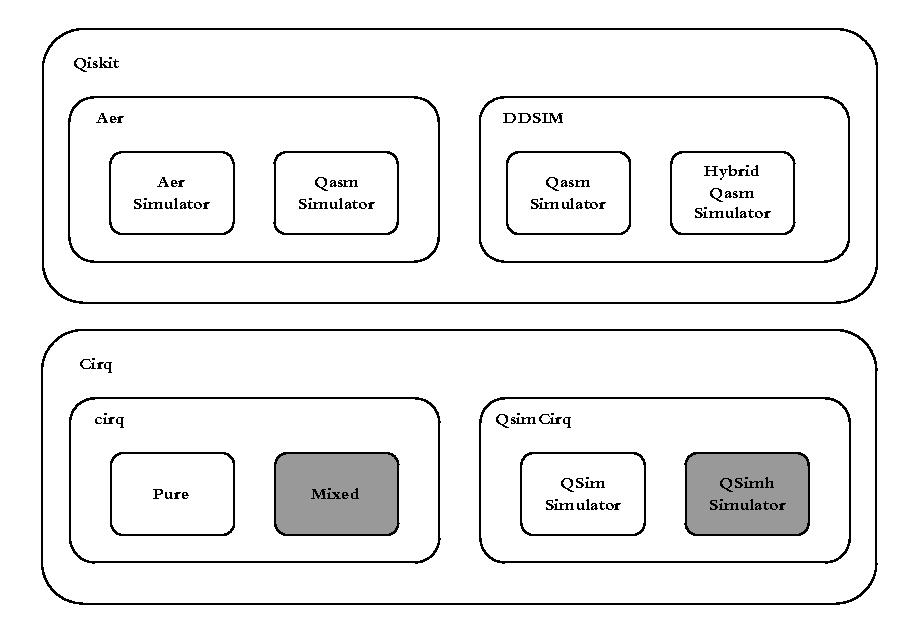
\includegraphics[scale=1]{images/backend_simulator_relation.pdf}
 	\caption[نمودار روابط پلتفرم‌ها و اجزای آن‌ها]{
 	نمودار روابط پلتفرم‌ها و اجزای آن‌ها (قسمت‌های خاکستری در پژوهش ما مورد بحث و بررسی نبوده‌اند.)
 	}
 	\label{fig:2}
 \end{figure}
 
\subsection{Qiskit}
 این پلتفرم توسط گروه تحقیقاتی IBM 
 \cite{javadi-abhari_quantum_2024}
 معرفی شده است که شامل چندین شبیه‌ساز با رویکردهای متفاوت شامل آن‌چه که در بخش
 \nameref{sec:simulators}
 گفته شده است. این پلتفرم علاوه بر شبیه‌ساز قابلیت‌هایی نظیر بهینه‌سازی و ترجمهٔ الگوریتم‌ها به زبان اسمبلی کوانتومی را نیز دارا است. علاوه‌برآن قابلیت اتصال به رایانه‌های واقعی کوانتومی ابری را نیز فراهم کرده است.
 
 هر پلتفرم برای جداسازی شبیه‌سازها باتوجه‌به رویکرد آن‌ها از بک‌اندهای متفاوت که همان لایه‌ای نرم‌افزاری باهدف چارچوب‌بندی به هر رویکرد شبیه‌سازی هستند، تشکیل شده است. در ادامه، شبیه‌سازها را به تفکیک بک‌اند، بررسی خواهیم کرد.
 
\subsubsection{Aer}
این بک‌اند شامل چهار شبیه‌ساز
\lr{AerSimulator}، \lr{QasmSimulator}، \lr{StatevectorSimulator} و \lr{UnitarySimulator}
است
\cite{javadi-abhari_quantum_2024}.
در پژوهش ما فقط به بررسی دو مورد اول پرداخته شده است.

\paragraph{:AerSimulator}
این شبیه‌ساز از چندین روش شبیه‌سازی و گزینه‌های قابل‌تنظیم برای هر روش شبیه‌سازی پشتیبانی می‌کند
\cite{noauthor_aersimulator_nodate}.
در محک این شبیه‌ساز، ابتدا الگوریتم‌های توضیح داده شده در بخش
\nameref{sec:algorithm_selection}
را اجرا و زمان اجرا و میزان حافظهٔ مصرفی آن را به تحریر نمودار درآورده‌ایم. نتیجهٔ حاصل شده در شکل‌های \ref{fig:3} و \ref{fig:4} نشانگر رفتار این شبیه‌ساز در اجرای الگوریتم‌های مختلف است.

از آن‌جایی که نتایج مربوط به الگوریتم Shor رفتار متفاوتی نسبت به دیگر الگوریتم‌ها داشته است، خروجی‌های مربوط به این الگوریتم در قالب جدول گزارش خواهد شد. این تفاوت در آن‌جایی است که برخلاف دیگر الگوریتم‌ها، داده‌های ورودی این الگوریتم محدودتر هستند و افزایش تعداد کیوبیت‌ها با افزایش عدد مرکب از دو عدد اول صورت می‌پذیرد. برای مثال در جدول \ref{tab:1} برای تجزیه‌ی عدد مرکب ۷۷ که از حاصل ضرب اعداد اول ۷ و ۱۱ بدست ‌می‌آید، الگوریتم Shor به ۲۴ کیوبیت احتیاج دارد تا بتواند این عدد را به عوامل اول آن تجزیه کند. به دلیل هم‌پوشانی که بین فاکتور‌های اول اعداد مرکب وجود دارد، نمی‌توان تعداد کیوبیت‌ها را یکی‌یکی افزایش داد و به همین دلیل زمان اجرا و حافظه‌ی مصرفی در قالب جداول نظیر جدول \ref{tab:1} گزارش شده است.

\begin{table}[h!]
	\centering
	\begin{LTR}
	\begin{tabular}{ |c|c|c|c| } 
		\hline
		\rl{عدد مرکب} & \rl{تعداد کیوبیت} & \rl{میانگین زمان اجرا (ثانیه)}  & \rl{میانگین حافظهٔ مصرفی (مگابایت)} \\
		\hline
		15 & 15 & 1.633536 & 121.723568 \\
		35 & 21 & 2.037188 & 122.529990 \\
		77 & 24 & 2.056493 & 125.207344 \\
		143 & 27 & 13.982873 & 129.990885 \\
		437 & 30 & N/A & N/A \\
		\hline
	\end{tabular}
	\end{LTR}
	\caption{
		جدول اطلاعات مربوط به اجرای الگوریتم Shor با
		\lr{Aer Simulator}
	}
	\label{tab:1}
\end{table}


\begin{figure}
	\centering
	\captionsetup{justification=centering}
	% This file was created with tikzplotlib v0.10.1.
\begin{tikzpicture}

	\definecolor{chocolate2267451}{RGB}{226,74,51}
	\definecolor{dimgray85}{RGB}{85,85,85}
	\definecolor{gainsboro229}{RGB}{229,229,229}
	\definecolor{gray119}{RGB}{119,119,119}
	\definecolor{lightgray204}{RGB}{204,204,204}
	\definecolor{mediumpurple152142213}{RGB}{152,142,213}
	\definecolor{sandybrown25119394}{RGB}{251,193,94}
	\definecolor{steelblue52138189}{RGB}{52,138,189}
	\definecolor{yellowgreen14218666}{RGB}{142,186,66}

	\begin{axis}[
    axis line style={black},
    tick style={black},
    grid=major,
    legend cell align={left},
    legend style={
        fill opacity=0.6,
        draw opacity=1,
        text opacity=1,
        at={(0.03,0.97)},
        anchor=north west,
        draw=lightgray204,
        fill=gainsboro229,
        font=\tiny,
        scale=0.1,
      },
    log basis y={10},
    tick align=outside,
    tick pos=left,
    x grid style={white},
    xlabel={\scriptsize\textcolor{black}{\rl{کیوبیت (عدد)}}},
    xmajorgrids,
    xmin=1, xmax=30,
    xtick distance=3,
    width=15cm,
    height=8cm,
    xtick style={color=dimgray85},
    y grid style={gray119},
    ylabel={\scriptsize\textcolor{black}{\rl{زمان اجرا (ثانیه)}}},
    ymajorgrids,
    ymin=0, ymax=3601,
    ymode=log,
    ytick style={color=dimgray85},
    ytick={1,10,100,1000,3600},
    yticklabels={
        \(\displaystyle {10^{0}}\),
        \(\displaystyle {10^{1}}\),
        \(\displaystyle {10^{2}}\),
        \(\displaystyle {10^{3}}\),
        \(\displaystyle {3600}\),
      },
    tick label style={font=\scriptsize}
  ]
		\addplot [semithick, chocolate2267451, dash pattern=on 1.5pt off 2.475pt, mark=*, mark size=3, mark options={solid}]
		table {%
				2 0.627046145969161
				3 0.620540094506347
				4 0.604433557288256
				5 0.557307506547704
				6 0.577668575013759
				7 0.619654589014544
				8 0.71398631361289
				9 0.808573271710126
				10 1.02579359791882
				11 1.70755112289388
				12 3.20736784415347
				13 7.18819421658966
				14 14.2466933424648
				15 35.4949261428393
				16 102.47516968324
				17 339.962429052473
				18 1280.15143594984
			};
		\addlegendentry{Deutsch-Jozsa (balanced)}
		\addplot [semithick, steelblue52138189, dash pattern=on 1.5pt off 2.475pt, mark=*, mark size=3, mark options={solid}]
		table {%
				2 0.619007757624548
				3 0.604727682732979
				4 0.599561547636613
				5 0.620342737456328
				6 0.58853850795581
				7 0.572819177000034
				8 0.603052117058198
				9 0.619279595640016
				10 0.576933875093806
				11 0.577723705664701
				12 0.600205244870589
				13 0.58294147643418
				14 0.553922971416598
				15 0.592418443107389
				16 0.610778429608383
				17 0.600022830768853
				18 0.590422668922574
				19 0.611738334022589
				20 0.654300124352312
				21 0.630325974868227
				22 0.63622559957729
				23 0.638434636725983
				24 0.597790644390853
				25 0.627876222588455
				26 0.608531387119575
				27 0.6158504437721
				28 0.617099424971479
			};
		\addlegendentry{Deutsch-Jozsa (constant)}
		\addplot [semithick, mediumpurple152142213, dash pattern=on 1.5pt off 2.475pt, mark=*, mark size=3, mark options={solid}]
		table {%
				2 0.625775995563965
				3 0.57775325457468
				4 0.600266677725543
				5 0.589891799900595
				6 0.587088828300655
				7 0.626464263387837
				8 0.583514458784009
				9 0.584047388728806
				10 0.622263500128114
				11 0.615194036042763
				12 0.598030297205431
				13 0.594709666634338
				14 0.627690367164237
				15 0.616887749775001
				16 0.595691669590584
				17 0.57740266146811
				18 0.571492576708758
				19 0.603566081606782
				20 0.606917118809959
				21 0.60262377817992
				22 0.593343016478124
				23 0.616170057293024
				24 0.61556207355751
				25 0.598909488495143
				26 0.597822427565701
				27 0.605887547693887
				28 0.627075332759571
			};
		\addlegendentry{Bernstein-Vazirani (basic)}
		\addplot [semithick, gray119, dash pattern=on 1.5pt off 2.475pt, mark=*, mark size=3, mark options={solid}]
		table {%
				2 0.573658010108471
				3 0.620933852126779
				4 0.565356786616637
				5 0.60226591831512
				6 0.603394420187709
				7 0.627239004985465
				8 0.622653529568651
				9 0.540358967517203
				10 0.577896496076911
				11 0.614049712703624
				12 0.578738785498038
				13 0.624202467350844
				14 0.607474514007616
				15 0.579391601718378
				16 0.583242387772462
				17 0.629852559202713
				18 0.70479680723381
				19 0.797260252629714
				20 0.900298026032862
				21 1.31753394724298
				22 2.10787159741243
				23 3.88590284328078
				24 7.52428175458831
				25 15.4287139293394
				26 31.9571831977387
				27 67.3291925381347
				28 142.335639079367
			};
		\addlegendentry{Quantum Fourier Transform (basic)}
		\addplot [semithick, sandybrown25119394, dash pattern=on 1.5pt off 2.475pt, mark=*, mark size=3, mark options={solid}]
		table {%
				2 2.20512034514554
				3 2.25890372158298
				4 2.20817412999522
				5 2.25658044806897
				6 2.23749479040781
				7 2.28594653873141
				8 2.29231295534857
				9 2.29971426264441
				10 2.263239687925
				11 2.30998097014085
				12 2.27261311829192
				13 2.26753437707271
				14 2.28446790319099
			};
		\addlegendentry{Simon (basic)}
		\addplot [semithick, yellowgreen14218666, dash pattern=on 1.5pt off 2.475pt, mark=*, mark size=3, mark options={solid}]
		table {%
				2 0.602772374542896
				3 0.635032709975031
				4 0.608714634228741
				5 0.606900246269116
				6 0.581898946577654
				7 0.589076310717568
				8 0.604531536341743
				9 0.612681784466321
				10 0.587272949534224
				11 0.604719892836494
				12 0.616668605208489
				13 0.556639777983306
				14 0.581914666579666
				15 0.598699448069502
				16 0.59577972315292
				17 0.615929523813299
				18 0.581640681853499
				19 0.676672037279193
				20 0.701376758362955
				21 0.844541243765989
				22 0.929530567222954
				23 1.2050532426835
				24 1.74018512284127
				25 3.02087841420321
				26 5.21255066366369
				27 10.796148155328
			};
		\addlegendentry{Grover (basic)}
	\end{axis}
\end{tikzpicture}

	\caption[نمودار زمان اجرا \lr{Aer Simulator}]{
		نمودار زمان اجرا بر حسب تعداد کیوبیت الگوریتم‌های مختلف در
		\lr{Aer Simulator}
		\newline \textit{
		توضیحات: دلیل عدم مشاهد‌هٔ واضح نمودار بعضی از الگوریتم‌ها، شباهت رفتاری شبیه‌ساز در اجرای آن‌ها است.
		}
		}
	\label{fig:3}
	\vspace{1cm}
	\captionsetup{justification=centering}
	% This file was created with tikzplotlib v0.10.1.
\begin{tikzpicture}

	\definecolor{chocolate2267451}{RGB}{226,74,51}
	\definecolor{dimgray85}{RGB}{85,85,85}
	\definecolor{gainsboro229}{RGB}{229,229,229}
	\definecolor{gray119}{RGB}{119,119,119}
	\definecolor{lightgray204}{RGB}{204,204,204}
	\definecolor{mediumpurple152142213}{RGB}{152,142,213}
	\definecolor{sandybrown25119394}{RGB}{251,193,94}
	\definecolor{steelblue52138189}{RGB}{52,138,189}
	\definecolor{yellowgreen14218666}{RGB}{142,186,66}

	\begin{axis}[
		axis line style={black},  
		tick style={black},  
		grid=major,  
		legend cell align={left},
		legend style={
				fill opacity=0.6,
				draw opacity=1,
				text opacity=1,
				at={(0.03,0.97)},
				anchor=north west,  
				draw=lightgray204,
				fill=gainsboro229,
				font=\tiny,
				scale=0.1,
			},
		log basis y={10},
		tick align=outside,
		tick pos=left,
		x grid style={white},
		xlabel={\scriptsize\textcolor{black}{\rl{کیوبیت (عدد)}}},  
		xmajorgrids,
		xmin=1, xmax=30,
		xtick distance=3,
		width=15cm,
		height=8cm,
		xtick style={color=dimgray85, },
		y grid style={gray119},
		ylabel={\scriptsize\textcolor{black}{\rl{مصرف حافظه (مگابایت)}}},  
		ymajorgrids,
		ymin=0, ymax=16385,
		ymode=log,
		ytick style={color=dimgray85},
		ytick={512,1024,10240,16384},
		yticklabels={
				\(\displaystyle {512}\),
				\(\displaystyle {1024}\),
				\(\displaystyle {10240}\),
				\(\displaystyle {16384}\),
			},
		tick label style={font=\scriptsize}
	]
		\addplot [semithick, chocolate2267451, dash pattern=on 1.5pt off 2.475pt, mark=*, mark size=3, mark options={solid}]
		table {%
				2 87.4186197916667
				3 87.44921875
				4 87.5455729166667
				5 87.8248697916667
				6 88.408203125
				7 88.4466145833333
				8 89.8626302083333
				9 92.5182291666667
				10 99.9869791666667
				11 116.418619791667
				12 148.608072916667
				13 219.912109375
				14 374.431640625
				15 696.547526041667
				16 1376.69661458333
				17 2812.40299479167
				18 5715.953125
			};
		\addlegendentry{Deutsch-Jozsa (balanced)}
		\addplot [semithick, steelblue52138189, dash pattern=on 1.5pt off 2.475pt, mark=*, mark size=3, mark options={solid}]
		table {%
				2 87.475
				3 87.175
				4 87.3484375
				5 87.38828125
				6 87.4828125
				7 87.121875
				8 87.43359375
				9 87.44140625
				10 87.5109375
				11 87.359375
				12 87.59609375
				13 87.4703125
				14 87.50546875
				15 87.428125
				16 87.50625
				17 87.2453125
				18 87.4296875
				19 87.6078125
				20 87.42265625
				21 87.6171875
				22 87.4046875
				23 87.29375
				24 87.76015625
				25 87.28125
				26 87.69765625
				27 87.740625
				28 87.54921875
			};
		\addlegendentry{Deutsch-Jozsa (constant)}
		\addplot [semithick, mediumpurple152142213, dash pattern=on 1.5pt off 2.475pt, mark=*, mark size=3, mark options={solid}]
		table {%
				2 87.2953125
				3 87.3328125
				4 87.55078125
				5 87.40078125
				6 87.10390625
				7 87.36875
				8 87.421875
				9 87.4109375
				10 87.20625
				11 87.48046875
				12 87.309375
				13 87.39609375
				14 87.10859375
				15 87.5421875
				16 87.3953125
				17 87.6125
				18 87.6265625
				19 87.70234375
				20 87.83359375
				21 88.01640625
				22 87.99140625
				23 88.0875
				24 88.040625
				25 87.72578125
				26 87.9578125
				27 87.96328125
				28 88.15625
			};
		\addlegendentry{Bernstein-Vazirani (basic)}
		\addplot [semithick, gray119, dash pattern=on 1.5pt off 2.475pt, mark=*, mark size=3, mark options={solid}]
		table {%
				2 86.9890625
				3 87.16640625
				4 87.26953125
				5 87.2453125
				6 87.54375
				7 87.415625
				8 87.484375
				9 87.85546875
				10 87.821875
				11 88.05078125
				12 88.1421875
				13 88.146875
				14 88.34453125
				15 88.67578125
				16 88.19921875
				17 88.58828125
				18 90.43203125
				19 94.90390625
				20 103.42109375
				21 119.759375
				22 152.7625
				23 216.6640625
				24 345.0125
				25 600.96171875
				26 1113.103125
				27 2136.6515625
				28 4184.44765625
			};
		\addlegendentry{Quantum Fourier Transform (basic)}
		\addplot [semithick, sandybrown25119394, dash pattern=on 1.5pt off 2.475pt, mark=*, mark size=3, mark options={solid}]
		table {%
				2 229.48359375
				3 229.76328125
				4 229.2375
				5 229.5859375
				6 229.3890625
				7 229.5078125
				8 229.37421875
				9 229.82578125
				10 230.20078125
				11 230.0484375
				12 229.82890625
				13 229.86953125
				14 230.175
			};
		\addlegendentry{Simon (basic)}
		\addplot [semithick, yellowgreen14218666, dash pattern=on 1.5pt off 2.475pt, mark=*, mark size=3, mark options={solid}]
		table {%
				2 87.5729166666667
				3 87.85546875
				4 87.86171875
				5 88.015625
				6 87.98671875
				7 87.853125
				8 87.88203125
				9 88.59921875
				10 88.46796875
				11 88.5484375
				12 88.64453125
				13 88.8578125
				14 89.4328125
				15 88.73203125
				16 88.7625
				17 88.6421875
				18 88.7015625
				19 102.64921875
				20 119.21484375
				21 151.7375
				22 215.79609375
				23 343.65859375
				24 599.646875
				25 1111.14453125
				26 2134.63359375
				27 4182.31484375
			};
		\addlegendentry{Grover (basic)}
	\end{axis}
\end{tikzpicture}

	\caption[نمودار مصرف حافظه \lr{Aer Simulator}]{
		نمودار مصرف حافظه بر حسب تعداد کیوبیت الگوریتم‌های مختلف
		\lr{Aer Simulator}
		\newline \textit{
			توضیحات: دلیل عدم مشاهد‌هٔ واضح نمودار بعضی از الگوریتم‌ها، شباهت رفتاری شبیه‌ساز در اجرای آن‌ها است.
		}
		}
	\label{fig:4}
\end{figure}

 از آن‌جایی که در محدودیت‌های این شبیه‌ساز تعداد ۳۲ کیوبیت ذکر شده همان‌طور که مشاهده می‌شود این شبیه‌ساز، در این محدوده، در اجرای همهٔ الگوریتم‌ها همان‌طور که انتظار می‌رود رفتار کرده است. دلیل این که محک با الگوریتمی نظیر Simon فقط تا ۱۶ کیوبیت ادامه پیدا کرده است این است که این الگوریتم برای حل مسئله به دوبرابر تعداد کیوبیت ورودی نیاز دارد. دیگر الگوریتم‌ها نظیر
 \lr{Grover}
 در تعداد کیوبیت کمتر رفتاری خطی و با افزایش تعداد کیوبیت رفتاری نمایی به خود می‌گیرند، طبق آن‌چه که در 
 \cite{jamadagni_benchmarking_2024}
 هم حدس زده شده است، امکان بهینه‌سازی غیر جامع این شبیه‌سازها به‌طوری‌که برای تعداد کیوبیت کمتر، بهینه شده باشند، وجود دارد.
  
  
\paragraph{:QasmSimulator}
این شبیه‌ساز هم از چندین روش شبیه‌سازی و اضافه‌کردن نویز به محاسبات پشتیبانی می‌کند. مانند قبل، اجرای الگوریتم‌ها با این شبیه‌ساز، در شکل‌ \ref{fig:5} برای زمان اجرا و در شکل \ref{fig:6} برای مصرف حافظه، آورده شده است.

\begin{figure}
	\centering
	\captionsetup{justification=centering}
	% This file was created with tikzplotlib v0.10.1.
\begin{tikzpicture}

	\definecolor{chocolate2267451}{RGB}{226,74,51}
	\definecolor{dimgray85}{RGB}{85,85,85}
	\definecolor{gainsboro229}{RGB}{229,229,229}
	\definecolor{gray119}{RGB}{119,119,119}
	\definecolor{lightgray204}{RGB}{204,204,204}
	\definecolor{mediumpurple152142213}{RGB}{152,142,213}
	\definecolor{sandybrown25119394}{RGB}{251,193,94}
	\definecolor{steelblue52138189}{RGB}{52,138,189}
	\definecolor{yellowgreen14218666}{RGB}{142,186,66}

	\begin{axis}[
    axis line style={black},
    tick style={black},
    grid=major,
    legend cell align={left},
    legend style={
        fill opacity=0.6,
        draw opacity=1,
        text opacity=1,
        at={(0.03,0.97)},
            anchor=north west,
        draw=lightgray204,
        fill=gainsboro229,
        font=\tiny,
        scale=0.1,
      },
    log basis y={10},
    tick align=outside,
    tick pos=left,
    x grid style={white},
    xlabel={\scriptsize\textcolor{black}{\rl{کیوبیت (عدد)}}},
    xmajorgrids,
    xmin=1, xmax=30,
    xtick distance=3,
    width=15cm,
    height=8cm,
    xtick style={color=dimgray85},
    y grid style={gray119},
    ylabel={\scriptsize\textcolor{black}{\rl{زمان اجرا (ثانیه)}}},
    ymajorgrids,
    ymin=0, ymax=3601,
    ymode=log,
    ytick style={color=dimgray85},
    ytick={1,10,100,1000,3600},
    yticklabels={
        \(\displaystyle {10^{0}}\),
        \(\displaystyle {10^{1}}\),
        \(\displaystyle {10^{2}}\),
        \(\displaystyle {10^{3}}\),
        \(\displaystyle {3600}\),
      },
    tick label style={font=\scriptsize}
  ]
		\addplot [semithick, chocolate2267451, dash pattern=on 1.5pt off 2.475pt, mark=*, mark size=3, mark options={solid}]
		table {%
				2 0.591304939326721
				3 0.618261231849203
				4 0.577479210922229
				5 0.628029825778719
				6 0.585005118487057
				7 0.599685080375904
				8 0.686506206148601
				9 0.757161041830157
				10 1.10488201718041
				11 1.75085018115432
				12 3.20639903344505
				13 7.15465083628399
				14 14.1702002220477
				15 35.5978986419106
				16 101.968037412245
				17 335.167788917545
				18 1284.39366972227
			};
		\addlegendentry{Deutsch-Jozsa (balanced)}
		\addplot [semithick, steelblue52138189, dash pattern=on 1.5pt off 2.475pt, mark=*, mark size=3, mark options={solid}]
		table {%
				2 0.551828144253206
				3 0.590439638488487
				4 0.567508328243958
				5 0.59823508426399
				6 0.621217404316689
				7 0.59946020230677
				8 0.586307117425776
				9 0.586612219671519
				10 0.607149356791602
				11 0.615608784099126
				12 0.587470683262726
				13 0.597111710344613
				14 0.632774829102299
				15 0.60417722842819
				16 0.598305650532505
				17 0.607249654493505
				18 0.596454103639309
				19 0.648430512579695
				20 0.610270239995572
				21 0.592256275573141
				22 0.591027687882309
				23 0.589262959065021
				24 0.601417301357851
				25 0.608057674837554
				26 0.594927006095338
				27 0.594472514747671
				28 0.612312020066186
			};
		\addlegendentry{Deutsch-Jozsa (constant)}
		\addplot [semithick, mediumpurple152142213, dash pattern=on 1.5pt off 2.475pt, mark=*, mark size=3, mark options={solid}]
		table {%
				2 0.629261635662515
				3 0.609867073800108
				4 0.572150678443529
				5 0.587133596952081
				6 0.604671435789041
				7 0.584635582594932
				8 0.622253316099649
				9 0.643627386165328
				10 0.634817802946494
				11 0.631513573105945
				12 0.581876545091362
				13 0.600967388597273
				14 0.633275790308154
				15 0.610229784309262
				16 0.617165758490921
				17 0.59918137634296
				18 0.575291403778686
				19 0.586644503646457
				20 0.592540540725066
				21 0.570599611521831
				22 0.609072857566842
				23 0.61669186193905
				24 0.610933927341243
				25 0.558536567458387
				26 0.579453378659335
				27 0.64195073023149
				28 0.607336142368001
			};
		\addlegendentry{Bernstein-Vazirani (basic)}
		\addplot [semithick, gray119, dash pattern=on 1.5pt off 2.475pt, mark=*, mark size=3, mark options={solid}]
		table {%
				2 0.563773031268817
				3 0.606310363437206
				4 0.626277882479424
				5 0.576788003446191
				6 0.582043068814394
				7 0.584138188967175
				8 0.556127427303879
				9 0.600190367513802
				10 0.61637415972298
				11 0.567178715037237
				12 0.609194127338951
				13 0.599344623938434
				14 0.605959790438121
				15 0.602827551586954
				16 0.597538671964051
				17 0.615186895679008
				18 0.686632744027427
				19 0.823638496072659
				20 0.98668141403423
				21 1.32044579789538
				22 2.15365708599401
				23 3.83974180395365
				24 7.56726772410653
				25 15.3069594878619
				26 32.1641921493779
				27 66.6852066668747
				28 142.767433474461
			};
		\addlegendentry{Quantum Fourier Transform (basic)}
		\addplot [semithick, sandybrown25119394, dash pattern=on 1.5pt off 2.475pt, mark=*, mark size=3, mark options={solid}]
		table {%
				2 2.25752379481232
				3 2.22970408734623
				4 2.22059319063216
				5 2.29589687441571
				6 2.24933181212165
				7 2.25391943622014
				8 2.28917567009626
				9 2.24331593991242
				10 2.25624203202973
				11 2.30272481055481
				12 2.30446695755306
				13 2.2845832516284
				14 2.31855734806885
			};
		\addlegendentry{Simon (basic)}
		\addplot [semithick, yellowgreen14218666, dash pattern=on 1.5pt off 2.475pt, mark=*, mark size=3, mark options={solid}]
		table {%
				2 0.649931628978543
				3 0.602191712238641
				4 0.579303999019014
				5 0.569967556803601
				6 0.608636965171304
				7 0.602942172379934
				8 0.628092795066265
				9 0.618951065669277
				10 0.593648011805128
				11 0.586805968356733
				12 0.626033275122053
				13 0.582294830908879
				14 0.596098828523707
				15 0.63659568658484
				16 0.632872437906449
				17 0.619900140388033
				18 0.580904288024011
				19 0.601640522692469
				20 0.67308033251598
				21 0.813011315558499
				22 0.901670418415067
				23 1.19198870973306
				24 1.69104096492784
				25 3.01485940653384
				26 5.22743925279817
				27 10.8084091084026
			};
		\addlegendentry{Grover (basic)}
	\end{axis}
\end{tikzpicture}

	\caption[نمودار زمان اجرا \lr{Qasm Simulator}]{
		نمودار زمان اجرا بر حسب تعداد کیوبیت الگوریتم‌های مختلف در 
		\lr{Qasm Simulator}
		\newline \textit{
			توضیحات: دلیل عدم مشاهد‌هٔ واضح نمودار بعضی از الگوریتم‌ها، شباهت رفتاری شبیه‌ساز در اجرای آن‌ها است.
		}
		}
	\label{fig:5}
	\vspace{1cm}
	\captionsetup{justification=centering}
	% This file was created with tikzplotlib v0.10.1.
\begin{tikzpicture}

	\definecolor{chocolate2267451}{RGB}{226,74,51}
	\definecolor{dimgray85}{RGB}{85,85,85}
	\definecolor{gainsboro229}{RGB}{229,229,229}
	\definecolor{gray119}{RGB}{119,119,119}
	\definecolor{lightgray204}{RGB}{204,204,204}
	\definecolor{mediumpurple152142213}{RGB}{152,142,213}
	\definecolor{sandybrown25119394}{RGB}{251,193,94}
	\definecolor{steelblue52138189}{RGB}{52,138,189}
	\definecolor{yellowgreen14218666}{RGB}{142,186,66}

	\begin{axis}[
		axis line style={black},  
		tick style={black},  
		grid=major,  
		legend cell align={left},
		legend style={
				fill opacity=0.6,
				draw opacity=1,
				text opacity=1,
				at={(0.03,0.97)},
				anchor=north west,  
				draw=lightgray204,
				fill=gainsboro229,
				font=\tiny,
				scale=0.1,
			},
		log basis y={10},
		tick align=outside,
		tick pos=left,
		x grid style={white},
		xlabel={\scriptsize\textcolor{black}{\rl{کیوبیت (عدد)}}},  
		xmajorgrids,
		xmin=1, xmax=30,
		xtick distance=3,
		width=15cm,
		height=8cm,
		xtick style={color=dimgray85, },
		y grid style={gray119},
		ylabel={\scriptsize\textcolor{black}{\rl{مصرف حافظه (مگابایت)}}},  
		ymajorgrids,
		ymin=0, ymax=16385,
		ymode=log,
		ytick style={color=dimgray85},
		ytick={512,1024,10240,16384},
		yticklabels={
				\(\displaystyle {512}\),
				\(\displaystyle {1024}\),
				\(\displaystyle {10240}\),
				\(\displaystyle {16384}\),
			},
		tick label style={font=\scriptsize}
	]
		\addplot [semithick, chocolate2267451, dash pattern=on 1.5pt off 2.475pt, mark=*, mark size=3, mark options={solid}]
		table {%
				2 87.5735677083333
				3 87.5924479166667
				4 87.6360677083333
				5 87.8001302083333
				6 88.2115885416667
				7 87.9498697916667
				8 89.7740885416667
				9 92.689453125
				10 99.71875
				11 116.413411458333
				12 148.22265625
				13 220.29296875
				14 378.317057291667
				15 691.319661458333
				16 1394.033203125
				17 2812.29557291667
				18 5734.58658854167
			};
		\addlegendentry{Deutsch-Jozsa (balanced)}
		\addplot [semithick, steelblue52138189, dash pattern=on 1.5pt off 2.475pt, mark=*, mark size=3, mark options={solid}]
		table {%
				2 87.19296875
				3 87.17265625
				4 87.303125
				5 87.41015625
				6 87.3859375
				7 87.459375
				8 87.3203125
				9 87.325
				10 87.23515625
				11 87.271875
				12 87.35078125
				13 87.3453125
				14 87.47265625
				15 87.31171875
				16 87.61484375
				17 87.3671875
				18 87.428125
				19 87.44921875
				20 87.709375
				21 87.45703125
				22 87.3140625
				23 87.4671875
				24 87.509375
				25 87.465625
				26 87.515625
				27 87.85078125
				28 87.7203125
			};
		\addlegendentry{Deutsch-Jozsa (constant)}
		\addplot [semithick, mediumpurple152142213, dash pattern=on 1.5pt off 2.475pt, mark=*, mark size=3, mark options={solid}]
		table {%
				2 87.2375
				3 87.02421875
				4 87.428125
				5 87.09453125
				6 87.3265625
				7 87.51328125
				8 87.28828125
				9 87.31484375
				10 87.47421875
				11 87.42734375
				12 87.478125
				13 87.19921875
				14 87.37265625
				15 87.8515625
				16 87.79375
				17 87.99140625
				18 87.7203125
				19 87.69296875
				20 87.7203125
				21 87.90859375
				22 88.07109375
				23 88.19609375
				24 88.13125
				25 88.20546875
				26 88.21171875
				27 88.0859375
				28 88.05078125
			};
		\addlegendentry{Bernstein-Vazirani (basic)}
		\addplot [semithick, gray119, dash pattern=on 1.5pt off 2.475pt, mark=*, mark size=3, mark options={solid}]
		table {%
				2 87.19375
				3 87.2796875
				4 87.21328125
				5 87.1296875
				6 87.484375
				7 87.4578125
				8 87.4359375
				9 87.871875
				10 88.00390625
				11 88.0015625
				12 88.09609375
				13 88.046875
				14 88.259375
				15 88.9859375
				16 88.07578125
				17 88.89140625
				18 88.85390625
				19 95.175
				20 103.3015625
				21 119.79609375
				22 152.88671875
				23 216.72890625
				24 345.0578125
				25 601.03203125
				26 1113.0140625
				27 2136.5984375
				28 4184.321875
			};
		\addlegendentry{Quantum Fourier Transform (basic)}
		\addplot [semithick, sandybrown25119394, dash pattern=on 1.5pt off 2.475pt, mark=*, mark size=3, mark options={solid}]
		table {%
				2 229.528125
				3 229.52578125
				4 229.37421875
				5 229.559375
				6 229.3640625
				7 229.47734375
				8 229.240625
				9 229.7171875
				10 229.85
				11 230.0359375
				12 230.13046875
				13 230.240625
				14 230.0828125
			};
		\addlegendentry{Simon (basic)}
		\addplot [semithick, yellowgreen14218666, dash pattern=on 1.5pt off 2.475pt, mark=*, mark size=3, mark options={solid}]
		table {%
				2 87.8736979166667
				3 87.93671875
				4 87.99296875
				5 88.325
				6 88.15703125
				7 88.21953125
				8 88.51015625
				9 88.32578125
				10 88.53671875
				11 88.53515625
				12 88.496875
				13 88.63046875
				14 89.03515625
				15 88.8109375
				16 88.92265625
				17 88.7890625
				18 90.925
				19 102.79375
				20 119.16953125
				21 151.8796875
				22 215.65234375
				23 343.571875
				24 599.48515625
				25 1111.06328125
				26 2134.353125
				27 4182.3015625
			};
		\addlegendentry{Grover (basic)}
	\end{axis}
\end{tikzpicture}

	\caption[نمودار مصرف حافظه \lr{Qasm Simulator}]{
		نمودار مصرف حافظه بر حسب تعداد کیوبیت الگوریتم‌های مختلف در
		\lr{Qasm Simulator}
		\newline \textit{
			توضیحات: دلیل عدم مشاهد‌هٔ واضح نمودار بعضی از الگوریتم‌ها، شباهت رفتاری شبیه‌ساز در اجرای آن‌ها است.
		}
		}
	\label{fig:6}
\end{figure}

از آن‌جایی که این دو شبیه‌ساز در یک بک‌اند توسعه داده شده‌اند، تفاوت چندانی در عملکرد آن‌ها مشاهده نمی‌شود و رفتار مشابهی را در مواجهه با الگوریتم‌های مختلف دارند که این رفتار موردانتظار از شبیه‌سازهای مدارهای کوانتومی است.

به صورت مجزا، عملکرد این شبیه‌ساز در اجرای الگوریتم Shor در جدول \ref{tab:2} گزارش شده است.
\begin{table}[h!]
	\centering
	\begin{LTR}
		\begin{tabular}{ |c|c|c|c| } 
			\hline
			\rl{عدد مرکب} & \rl{تعداد کیوبیت} & \rl{میانگین زمان اجرا (ثانیه)}  & \rl{میانگین حافظهٔ مصرفی (مگابایت)} \\
			\hline
			15 & 15 & 1.770852 & 121.732682 \\
			35 & 21 & 3.714265 & 123.226562 \\
			77 & 24 & 2.542166 & 125.411875 \\
			143 & 27 & 14.051529 & 130.393229 \\
			437 & 30 & N/A & N/A \\
			\hline
		\end{tabular}
	\end{LTR}
	\caption{
		جدول اطلاعات مربوط به اجرای الگوریتم Shor با
		\lr{Qasm Simulator}
	}
	\label{tab:2}
\end{table}
 
\subsubsection{DDSIM}
این بک‌اند چهارچوبی برای شبیه‌سازها تعیین کرده است که از یک روش مبتنی بر گراف، به‌ویژه نمودارهای تصمیم‌گیری، برای شبیه‌سازی کارآمد مدارهای کوانتومی استفاده می‌کند و به‌جای ذخیره بردارها و ماتریس‌های بزرگی که به‌صورت نمایی رشد می‌کنند، از این نمودارها برای ثبت تکرارهای موجود در محاسبات بهره می‌برد. در واقع به نحوی از برنامه‌نویسی پویا برای بهبود کارایی شبیه‌سازی استفاده می‌کند و به‌این‌ترتیب استفاده از حافظه را به میزان قابل‌توجهی کاهش می‌دهد. عملیات کوانتومی از طریق ضرب ماتریس‌ها و بردارها در این قالب به‌صورت بازگشتی انجام می‌شوند بدون این که نیاز باشد کل آن‌ها پردازش شوند. اندازه‌گیری نیز به همین شکل انجام می‌شود و تغییرات حالت به طور کارآمد در نمودارها نمایش داده می‌شود. این روش باعث می‌شود که این نوع از شبیه‌سازها در مقایسه با شبیه‌سازهای دیگر، عملکرد بهتری داشته باشند و بتوانند تعداد بیش‌تری کیوبیت را مدیریت کنند و زمان و حافظهٔ محاسباتی کمتری مصرف کنند 
\cite{zulehner_advanced_2019}.
\paragraph{:QasmSimulator}
این شبیه‌ساز از روش Schrödinger استفاده می‌کند که بر اساس نمودارهای تصمیم‌گیری به‌عنوان یک ساختمان داده، طراحی شده و می‌توان از آن برای به‌دست‌آوردن بردار حالت کامل مدار کوانتومی «شبیه‌سازی قوی» 
\cite{zulehner_advanced_2019}
و یا نمونه‌گیری از توزیع خروجی یک مدار کوانتومی «شبیه‌سازی ضعیف» 
\cite{hillmich_just_2020}
بهره برد. برای این منظور، شبیه‌ساز با نمایش نمودار تصمیم‌گیری از حالت اولیه آغاز می‌شود و سپس در هر مرحله، گیت‌های مدار را یکی‌یکی اعمال می‌کند. نمایش نمودار تصمیم‌گیری از بردار حالت در هر مرحله به‌روزرسانی می‌شود. این شبیه‌ساز قادر است مدارهای کوانتومی تقریباً دلخواه، از جمله مدارهایی با اندازه‌گیری‌ها و بازتنظیم‌های میانی را مدیریت کند. برای مدارهایی که شامل عملیات غیر واحدی (به‌جز اندازه‌گیری‌ها در انتهای مدار) نیستند، شبیه‌سازی فقط یک‌بار انجام می‌شود. در این حالت، تعداد نمونه‌های درخواستی به طور متعاقب از نمودار تصمیم‌گیری نهایی گرفته می‌شود که منجر به زمان اجرای سریع شبیه‌سازی می‌گردد.

شایان‌ذکر است که این شبیه‌ساز با شبیه‌سازی که در قسمت قبل توضیح داده شده است، متفاوت است. با این که هر دو از روش Schrödinger برای شبیه‌سازی بهره گرفته‌اند؛ اما ساختمان داده‌ای که در شبیه‌ساز دوم با بک‌اند DDSIM توسعه‌یافته به طور کامل با شبیه‌ساز با بک‌اند Aer متفاوت است.

\begin{figure}
	\centering
	\captionsetup{justification=centering}
	% This file was created with tikzplotlib v0.10.1.
\begin{tikzpicture}

	\definecolor{chocolate2267451}{RGB}{226,74,51}
	\definecolor{dimgray85}{RGB}{85,85,85}
	\definecolor{gainsboro229}{RGB}{229,229,229}
	\definecolor{gray119}{RGB}{119,119,119}
	\definecolor{lightgray204}{RGB}{204,204,204}
	\definecolor{mediumpurple152142213}{RGB}{152,142,213}
	\definecolor{sandybrown25119394}{RGB}{251,193,94}
	\definecolor{steelblue52138189}{RGB}{52,138,189}

	\begin{axis}[
    axis line style={black},
    tick style={black},
    grid=major,
    legend cell align={left},
    legend style={
        fill opacity=0.6,
        draw opacity=1,
        text opacity=1,
        at={(0.03,0.97)},
            anchor=north west,
        draw=lightgray204,
        fill=gainsboro229,
        font=\tiny,
        scale=0.1,
      },
    log basis y={10},
    tick align=outside,
    tick pos=left,
    x grid style={white},
    xlabel={\scriptsize\textcolor{black}{\rl{کیوبیت (عدد)}}},
    xmajorgrids,
    xmin=1, xmax=30,
    xtick distance=3,
    width=15cm,
    height=8cm,
    xtick style={color=dimgray85},
    y grid style={gray119},
    ylabel={\scriptsize\textcolor{black}{\rl{زمان اجرا (ثانیه)}}},
    ymajorgrids,
    ymin=0, ymax=3601,
    ymode=log,
    ytick style={color=dimgray85},
    ytick={1,10,100,1000,3600},
    yticklabels={
        \(\displaystyle {10^{0}}\),
        \(\displaystyle {10^{1}}\),
        \(\displaystyle {10^{2}}\),
        \(\displaystyle {10^{3}}\),
        \(\displaystyle {3600}\),
      },
    tick label style={font=\scriptsize}
  ]
		\addplot [semithick, chocolate2267451, dash pattern=on 1.5pt off 2.475pt, mark=*, mark size=3, mark options={solid}]
		table {%
				2 0.612252539865214
				3 0.601244009112429
				4 0.593100177356242
				5 0.599033548432153
				6 0.588201006522595
				7 0.696863817125534
				8 0.807233468592781
				9 1.13087342554267
				10 1.71884750350639
				11 3.10042611536326
				12 6.16515288339251
				13 13.8144959049632
				14 33.8972658858413
				15 92.8064641957886
				16 276.278772114309
				17 957.045420053034
			};
		\addlegendentry{Deutsch-Jozsa (balanced)}
		\addplot [semithick, steelblue52138189, dash pattern=on 1.5pt off 2.475pt, mark=*, mark size=3, mark options={solid}]
		table {%
				2 0.581679406032504
				3 0.583822387977432
				4 0.554115560236107
				5 0.604149132044441
				6 0.625254636644959
				7 0.620841372833219
				8 0.603722554715012
				9 0.621960763666647
				10 0.555654150495092
				11 0.616124791177196
				12 0.607931797965015
				13 0.597951840958091
				14 0.599682196553941
				15 0.592530303824046
				16 0.598625423020701
				17 0.593269360834072
				18 0.599336407179625
				19 0.587269851931074
				20 0.574376530453162
				21 0.620605356850644
				22 0.612003996071707
				23 0.614884185756279
				24 0.593040984237245
				25 0.585609606902293
				26 0.584196067951382
				27 0.593606885921734
				28 0.595821913605421
				29 0.62102413421069
			};
		\addlegendentry{Deutsch-Jozsa (constant)}
		\addplot [semithick, mediumpurple152142213, dash pattern=on 1.5pt off 2.475pt, mark=*, mark size=3, mark options={solid}]
		table {%
				2 0.587890294405024
				3 0.607217057347551
				4 0.594140859327094
				5 0.608088254226921
				6 0.570405318564412
				7 0.611789878501847
				8 0.625440780474689
				9 0.628608712815088
				10 0.594298879911107
				11 0.61193676720635
				12 0.569981662448604
				13 0.56787768890125
				14 0.596789004360342
				15 0.625093936909044
				16 0.580766247407487
				17 0.588977490424729
				18 0.599994484817433
				19 0.585004511304591
				20 0.621772335048289
				21 0.627481898696414
				22 0.617059661434273
				23 0.605341294828682
				24 0.601486240354653
				25 0.564193096421025
				26 0.595621089723595
				27 0.606451361787534
				28 0.606056650122247
				29 0.631891646089077
			};
		\addlegendentry{Bernstein-Vazirani (basic)}
		\addplot [semithick, gray119, dash pattern=on 1.5pt off 2.475pt, mark=*, mark size=3, mark options={solid}]
		table {%
				2 1.02784112379512
				3 0.610807095489116
				4 0.609624942989935
				5 0.593514286111592
				6 0.58695403577948
				7 0.589214627628456
				8 0.600340207582892
				9 0.616284045165562
				10 0.616076385429282
				11 0.603170323702486
				12 0.594240256305975
				13 0.626532288466614
				14 0.598152303267251
				15 0.6351940589673
				16 0.699118805171104
				17 0.720838692816472
				18 0.817515612120289
				19 0.9790566556133
				20 1.10810050962505
				21 1.78353961277023
				22 2.44386672673494
				23 4.62526021299006
				24 9.7430977261344
				25 18.1854031520582
				26 37.1694594946284
				27 64.7092330153807
				28 146.479316623025
				29 280.034649538871
			};
		\addlegendentry{Quantum Fourier Transform (basic)}
		\addplot [semithick, sandybrown25119394, dash pattern=on 1.5pt off 2.475pt, mark=*, mark size=3, mark options={solid}]
		table {%
				2 0.591846040119179
				3 0.630324380985934
				4 0.570937748298535
				5 0.596453599062918
				6 0.613574608037819
				7 0.596186930927414
				8 0.603409369202958
				9 0.652565426564348
				10 0.618473927028231
				11 0.575762926989485
				12 0.605624820432406
				13 0.626369027859028
				14 0.632398366185987
				15 0.632420712927039
				16 0.616576239492234
				17 0.633317724737592
				18 0.617690554121882
				19 0.631588403936496
				20 0.615689365074128
				21 0.631977333883819
				22 0.589721571302832
				23 0.592716939375255
				24 0.603072703158856
				25 0.592843291320397
				26 0.589109646095748
				27 0.646674980634838
				28 0.636228435303491
				29 0.57088168193142
			};
		\addlegendentry{Grover (basic)}
	\end{axis}
\end{tikzpicture}

	\caption[نمودار زمان اجرا \lr{DDSIM Qasm Simulator}]{
		نمودار زمان اجرا بر حسب تعداد کیوبیت الگوریتم‌های مختلف در
		\lr{DDSIM Qasm Simulator}
		\newline \textit{
			توضیحات: دلیل عدم مشاهد‌هٔ واضح نمودار بعضی از الگوریتم‌ها، شباهت رفتاری شبیه‌ساز در اجرای آن‌ها است.
		}
		}
	\label{fig:7}
	\vspace{1cm}
	\captionsetup{justification=centering}
	% This file was created with tikzplotlib v0.10.1.
\begin{tikzpicture}

	\definecolor{chocolate2267451}{RGB}{226,74,51}
	\definecolor{dimgray85}{RGB}{85,85,85}
	\definecolor{gainsboro229}{RGB}{229,229,229}
	\definecolor{gray119}{RGB}{119,119,119}
	\definecolor{lightgray204}{RGB}{204,204,204}
	\definecolor{mediumpurple152142213}{RGB}{152,142,213}
	\definecolor{sandybrown25119394}{RGB}{251,193,94}
	\definecolor{steelblue52138189}{RGB}{52,138,189}

	\begin{axis}[
    axis line style={black},  
    tick style={black},  
    grid=major,  
    legend cell align={left},
    legend style={
        fill opacity=0.6,
        draw opacity=1,
        text opacity=1,
        at={(0.03,0.97)},
            anchor=north west,  
        draw=lightgray204,
        fill=gainsboro229,
        font=\tiny,
        scale=0.1,
      },
    log basis y={10},
    tick align=outside,
    tick pos=left,
    x grid style={white},
    xlabel={\scriptsize\textcolor{black}{\rl{کیوبیت (عدد)}}},  
    xmajorgrids,
    xmin=1, xmax=30,
    xtick distance=3,
    width=15cm,
    height=8cm,
    xtick style={color=dimgray85, },
    y grid style={gray119},
    ylabel={\scriptsize\textcolor{black}{\rl{مصرف حافظه (مگابایت)}}},  
    ymajorgrids,
    ymin=0, ymax=16385,
    ymode=log,
    ytick style={color=dimgray85},
    ytick={512,1024,10240,16384},
    yticklabels={
        \(\displaystyle {512}\),
        \(\displaystyle {1024}\),
        \(\displaystyle {10240}\),
        \(\displaystyle {16384}\),
      },
    tick label style={font=\scriptsize}
  ]
		\addplot [semithick, chocolate2267451, dash pattern=on 1.5pt off 2.475pt, mark=*, mark size=3, mark options={solid}]
		table {%
				2 87.8625
				3 87.86796875
				4 87.8390625
				5 87.95234375
				6 97.40234375
				7 89.33828125
				8 90.4515625
				9 91.82734375
				10 99.365625
				11 136.46328125
				12 152.90703125
				13 179.47734375
				14 231.49375
				15 345.29375
				16 617.43828125
				17 1206.96875
			};
		\addlegendentry{Deutsch-Jozsa (balanced)}
		\addplot [semithick, steelblue52138189, dash pattern=on 1.5pt off 2.475pt, mark=*, mark size=3, mark options={solid}]
		table {%
				2 87.95703125
				3 87.70390625
				4 87.85390625
				5 87.9203125
				6 87.86640625
				7 87.6640625
				8 87.7734375
				9 88.0140625
				10 87.88046875
				11 87.8296875
				12 87.9625
				13 87.78671875
				14 88.1328125
				15 87.8359375
				16 87.809375
				17 87.82890625
				18 88.0640625
				19 87.96875
				20 87.96796875
				21 87.83671875
				22 88.2640625
				23 88.07890625
				24 88.2703125
				25 88.33515625
				26 88.24375
				27 88.396875
				28 88.4890625
				29 88.5140625
			};
		\addlegendentry{Deutsch-Jozsa (constant)}
		\addplot [semithick, mediumpurple152142213, dash pattern=on 1.5pt off 2.475pt, mark=*, mark size=3, mark options={solid}]
		table {%
				2 87.9140625
				3 87.8359375
				4 87.79296875
				5 87.75078125
				6 88.0078125
				7 87.8359375
				8 87.7359375
				9 88.16640625
				10 87.846875
				11 87.9
				12 87.76484375
				13 87.6921875
				14 88.37578125
				15 87.90546875
				16 88.31484375
				17 88.121875
				18 88.61484375
				19 88.55625
				20 88.121875
				21 88.53046875
				22 88.225
				23 88.41328125
				24 88.34453125
				25 88.4953125
				26 88.54140625
				27 88.3859375
				28 88.128125
				29 88.51484375
			};
		\addlegendentry{Bernstein-Vazirani (basic)}
		\addplot [semithick, gray119, dash pattern=on 1.5pt off 2.475pt, mark=*, mark size=3, mark options={solid}]
		table {%
				2 87.4109375
				3 87.709375
				4 87.65078125
				5 87.6453125
				6 87.6484375
				7 87.9546875
				8 87.60234375
				9 88.16875
				10 87.87890625
				11 88.221875
				12 88.084375
				13 90.8375
				14 110.4453125
				15 105.90078125
				16 110.46171875
				17 105.2296875
				18 110.0625
				19 111.4046875
				20 109.04296875
				21 111.61953125
				22 111.54453125
				23 111.85859375
				24 111.8578125
				25 112.89765625
				26 112.9390625
				27 113.35546875
				28 114.05
				29 113.60234375
			};
		\addlegendentry{Quantum Fourier Transform (basic)}
		\addplot [semithick, sandybrown25119394, dash pattern=on 1.5pt off 2.475pt, mark=*, mark size=3, mark options={solid}]
		table {%
				2 88.1015625
				3 88.1497395833333
				4 88.587890625
				5 88.3330078125
				6 88.728125
				7 88.615625
				8 88.19609375
				9 88.05
				10 88.440625
				11 88.16484375
				12 88.69140625
				13 88.72578125
				14 88.44921875
				15 88.31640625
				16 88.490625
				17 88.41953125
				18 88.65859375
				19 88.853125
				20 88.72734375
				21 93.07109375
				22 91.23359375
				23 88.70546875
				24 88.6734375
				25 90.375
				26 88.58125
				27 88.71953125
				28 88.53671875
				29 88.69609375
			};
		\addlegendentry{Grover (basic)}
	\end{axis}
\end{tikzpicture}

	\caption[نمودار مصرف حافظه \lr{DDSIM Qasm Simulator}]{
		نمودار مصرف حافظه بر حسب تعداد کیوبیت الگوریتم‌های مختلف در
		\lr{DDSIM Qasm Simulator}
		\newline \textit{
			توضیحات: دلیل عدم مشاهد‌هٔ واضح نمودار بعضی از الگوریتم‌ها، شباهت رفتاری شبیه‌ساز در اجرای آن‌ها است.
		}
		}
	\label{fig:8}
\end{figure}

شکل‌های \ref{fig:7} و \ref{fig:8} رفتار این شبیه‌ساز را نسبت به الگوریتم‌های مختلف نشان می‌دهد که به‌طورکلی در مقایسه با شبیه‌ساز Aer در زمان اجرا و حافظهٔ کمتری شبیه‌سازی‌ها را انجام داده است که این خود نقطه‌ی قوت این شبیه‌ساز را نشان می‌دهد و این بهبود برای محققانی که قصد اجرای شبیه‌سازها بر روی رایانه‌های شخصی را دارند بسیار مؤثر خواهد بود. همان‌طور که در بخش‌های قبل گفته شد، پیاده‌سازی الگوریتم
\lr{Simon}،
به دلیل عدم وجود ویژگی ذخیرهٔ نتایج اجرای الگوریتم‌ها، در این بک‌اند انجام نشده است و به همین دلیل در نمودارهای ذکر شده، اطلاعاتی مربوط به الگوریتم Simon وجود ندارد.

با تفاوت‌‌های ذکرشده در ساختار الگوریتم Shor و تفاوت‌های آن با دیگر محک‌ها، عملکرد این شبیه‌ساز در اجرای این الگوریتم به صورت مجزا در جدول \ref{tab:3} گزارش شده است. رفتار این شبیه‌ساز در اجرای این الگوریتم با افزایش از ۲۱ کیوبیت به ۲۴ کیوبیت، غیرقابل انتظار بوده است چرا که انتظار بر این است با افزایش تعداد کیوبیت زمان اجرا و میزان مصرف حافظه هم افزایش یابد. در توجیه این رفتار، از آن‌جایی که الگوریتم Shor در مراحل خود به صورت احتمالی به پاسخ می‌رسد، رسیدن به پاسخ در زمان محدودشده در آزمایش‌ها (۳۶۰۰ ثانیه برای هر اجرا) امکان‌پذیر نبوده است. این در حالی است که هر اجرا به بیش از ۵ بار تکرار انجام شده است. در نتیجه این کاهش زمان در قبال نرسیدن به پاسخ نهایی بوده است.
\begin{table}[h!]
	\centering
	\begin{LTR}
		\begin{tabular}{ |c|c|c|c| } 
			\hline
			\rl{عدد مرکب} & \rl{تعداد کیوبیت} & \rl{میانگین زمان اجرا (ثانیه)}  & \rl{میانگین حافظهٔ مصرفی (مگابایت)} \\
			\hline
			15 & 15 & 1.643833 & 124.590885 \\
			35 & 21 & 3.008140 & 131.823495 \\
			77 & 24 & 1.883989 & 128.149063 \\
			143 & 27 & 6.765308 & 147.167188 \\
			437 & 30 & N/A & N/A \\
			\hline
		\end{tabular}
	\end{LTR}
	\caption{
		جدول اطلاعات مربوط به اجرای الگوریتم Shor با
		\lr{DDSIM Qasm Simulator}
	}
	\label{tab:3}
\end{table}

\paragraph{\lr{:Hybrid QasmSimulator}}
این مدل شبیه‌ساز از رویکرد ترکیبی
\lr{Schrödinger-Feynman}
استفاده می‌کند به‌طوری‌که از تمام حافظه و واحدهای پردازشی موجود برای شبیه‌سازی کارآمد مدارهای کوانتومی بهره ببرد. در شبیه‌سازی‌هایی که به سبک Schrödinger هستند با محدودیت‌های حافظه مواجه می‌شوند و یا در شبیه‌سازی‌های به سبک Feynman مدت‌زمان بسیار زیادی نیاز دارند، این شبیه‌ساز سعی می‌کند با ایجاد یک مصالحه بین الزامات حافظه و زمان اجرا بهترین شبیه‌سازی ممکن، وابسته به مدار کوانتومی ورودی را ارائه دهد
 \cite{noauthor_hybrid_nodate}.
 
 شکل‌های \ref{fig:9} و \ref{fig:10} رفتار این شبیه‌ساز را نسبت به الگوریتم‌های مختلف نشان می‌دهد. از آن‌جایی که این مدل شبیه‌ساز در مراحل اولیهٔ توسعهٔ خود قرار دارد، این احتمال وجود دارد که انتخاب بین استفاده از رویکردهای یاد شده، باعث چنین ناهمواری‌هایی در نمودار زمان اجرا و حافظه شود. در کل، بدون در نظر گرفتن وقت صرف شده برای توسعهٔ شبیه‌سازهای مختلف، این شبیه‌ساز عملکرد خوبی نسبت به شبیه‌سازهایی که تاکنون شرح داده شده‌اند، نداشته است.

\begin{figure}
	\centering
	\captionsetup{justification=centering}
	% This file was created with tikzplotlib v0.10.1.
\begin{tikzpicture}

	\definecolor{chocolate2267451}{RGB}{226,74,51}
	\definecolor{dimgray85}{RGB}{85,85,85}
	\definecolor{gainsboro229}{RGB}{229,229,229}
	\definecolor{gray119}{RGB}{119,119,119}
	\definecolor{lightgray204}{RGB}{204,204,204}
	\definecolor{mediumpurple152142213}{RGB}{152,142,213}
	\definecolor{sandybrown25119394}{RGB}{251,193,94}
	\definecolor{steelblue52138189}{RGB}{52,138,189}

	\begin{axis}[
    axis line style={black},
    tick style={black},
    grid=major,
    legend cell align={left},
    legend style={
        fill opacity=0.6,
        draw opacity=1,
        text opacity=1,
        at={(0.97,0.97)},
        anchor=north east,
        draw=lightgray204,
        fill=gainsboro229,
        font=\tiny,
        scale=0.1,
      },
    log basis y={10},
    tick align=outside,
    tick pos=left,
    x grid style={white},
    xlabel={\scriptsize\textcolor{black}{\rl{کیوبیت (عدد)}}},
    xmajorgrids,
    xmin=1, xmax=30,
    xtick distance=3,
    width=15cm,
    height=8cm,
    xtick style={color=dimgray85},
    y grid style={gray119},
    ylabel={\scriptsize\textcolor{black}{\rl{زمان اجرا (ثانیه)}}},
    ymajorgrids,
    ymin=0, ymax=3601,
    ymode=log,
    ytick style={color=dimgray85},
    ytick={1,10,100,1000,3600},
    yticklabels={
        \(\displaystyle {10^{0}}\),
        \(\displaystyle {10^{1}}\),
        \(\displaystyle {10^{2}}\),
        \(\displaystyle {10^{3}}\),
        \(\displaystyle {3600}\),
      },
    tick label style={font=\scriptsize}
  ]
		\addplot [semithick, chocolate2267451, dash pattern=on 1.5pt off 2.475pt, mark=*, mark size=3, mark options={solid}]
		table {%
				2 0.597868566396571
				6 0.937824552238864
				7 1.92104576240808
				8 5.9681933120616
				9 21.3897546774469
				10 82.1233237829238
				11 334.310288762949
			};
		\addlegendentry{Deutsch-Jozsa (balanced)}
		\addplot [semithick, steelblue52138189, dash pattern=on 1.5pt off 2.475pt, mark=*, mark size=3, mark options={solid}]
		table {%
				2 0.693353301867182
				3 0.636428528960232
				4 0.543177408027685
				5 0.621790375881577
				6 0.60925448196725
				7 0.576636772212676
				8 0.610487772751591
				9 0.585676123126805
				10 0.584691701436717
				11 0.594200421498198
				12 0.604266198276102
				13 0.608911082266084
				14 0.626623257599496
				15 0.59508719711376
				16 0.573776808624804
				17 0.606440932432929
				18 0.620692065670245
				19 0.623131562941646
				20 0.710584894287226
				21 0.703167336558315
				22 0.953626509743707
				23 1.10023575912188
				24 1.64030202724372
				25 2.70312382158595
				26 4.75195973066357
			};
		\addlegendentry{Deutsch-Jozsa (constant)}
		\addplot [semithick, mediumpurple152142213, dash pattern=on 1.5pt off 2.475pt, mark=*, mark size=3, mark options={solid}]
		table {%
				2 0.581378518886505
				3 0.623281716272181
				4 0.596886265077828
				5 0.599966782263141
				6 0.584264622743482
				7 0.566233540964989
				8 0.542885204059641
				9 0.587834644726815
				10 0.588105452066124
				11 0.641619736953297
				12 0.595353376518755
				13 0.627206856614325
				14 0.651481216905507
				15 0.658358243154701
				16 0.646803615414515
				17 0.681878867209783
				18 0.700563510029233
				19 0.744875336952375
				20 0.80435271212688
				21 1.00897318390555
				22 1.27306003520674
				23 1.75283078873344
				24 2.79774983295597
				25 4.9588869399558
			};
		\addlegendentry{Bernstein-Vazirani (basic)}
		\addplot [semithick, gray119, dash pattern=on 1.5pt off 2.475pt, mark=*, mark size=3, mark options={solid}]
		table {%
				2 0.57742029532998
				3 0.641968571283478
				4 0.684351089396766
				5 2.83788407148147
				6 152.468731147669
				12 0.966184949275977
				13 1100.93839546889
				16 0.713509314210841
				17 113.161398924993
				20 1.34196857035549
				23 4.95272919842685
			};
		\addlegendentry{Quantum Fourier Transform (basic)}
		\addplot [semithick, sandybrown25119394, dash pattern=on 1.5pt off 2.475pt, mark=*, mark size=3, mark options={solid}]
		table {%
				2 0.605223086361549
				3 0.604693105969172
				4 0.609341761052035
				5 0.579868231132997
				6 0.617290399830352
				7 0.569949517674462
				8 0.618231423822473
				9 0.590279338170018
				10 0.620839491666611
				11 0.580937174826352
				12 0.606015417502191
				13 0.584184406072495
				14 0.574784896681935
				15 0.598159480306858
				16 0.711619082398483
				17 0.704890572807915
				18 0.679538464290166
				19 0.826914913741584
				20 1.13363334540886
				21 1.40032311181396
				22 2.42980830508291
				23 3.63360355332663
				24 7.82735892188922
				25 12.6515511293194
			};
		\addlegendentry{Grover (basic)}
	\end{axis}
\end{tikzpicture}

	\caption[نمودار زمان اجرا \lr{DDSIM Hybrid Qasm Simulator}]{
		نمودار زمان اجرا بر حسب تعداد کیوبیت الگوریتم‌های مختلف در
		\lr{DDSIM Hybrid Qasm Simulator}
		\newline \textit{
			توضیحات: دلیل عدم مشاهد‌هٔ واضح نمودار بعضی از الگوریتم‌ها، شباهت رفتاری شبیه‌ساز در اجرای آن‌ها است.
		}
	}
	\label{fig:9}
	\vspace{1cm}
	\captionsetup{justification=centering}
	% This file was created with tikzplotlib v0.10.1.
\begin{tikzpicture}

	\definecolor{chocolate2267451}{RGB}{226,74,51}
	\definecolor{dimgray85}{RGB}{85,85,85}
	\definecolor{gainsboro229}{RGB}{229,229,229}
	\definecolor{gray119}{RGB}{119,119,119}
	\definecolor{lightgray204}{RGB}{204,204,204}
	\definecolor{mediumpurple152142213}{RGB}{152,142,213}
	\definecolor{sandybrown25119394}{RGB}{251,193,94}
	\definecolor{steelblue52138189}{RGB}{52,138,189}

	\begin{axis}[
    axis line style={black},  
    tick style={black},  
    grid=major,  
    legend cell align={left},
    legend style={
        fill opacity=0.6,
        draw opacity=1,
        text opacity=1,
        at={(0.03,0.97)},
            anchor=north west,  
        draw=lightgray204,
        fill=gainsboro229,
        font=\tiny,
        scale=0.1,
      },
    log basis y={10},
    tick align=outside,
    tick pos=left,
    x grid style={white},
    xlabel={\scriptsize\textcolor{black}{\rl{کیوبیت (عدد)}}},  
    xmajorgrids,
    xmin=1, xmax=30,
    xtick distance=3,
    width=15cm,
    height=8cm,
    xtick style={color=dimgray85, },
    y grid style={gray119},
    ylabel={\scriptsize\textcolor{black}{\rl{مصرف حافظه (مگابایت)}}},  
    ymajorgrids,
    ymin=0, ymax=16385,
    ymode=log,
    ytick style={color=dimgray85},
    ytick={512,1024,10240,16384},
    yticklabels={
        \(\displaystyle {512}\),
        \(\displaystyle {1024}\),
        \(\displaystyle {10240}\),
        \(\displaystyle {16384}\),
      },
    tick label style={font=\scriptsize}
  ]
		\addplot [semithick, chocolate2267451, dash pattern=on 1.5pt off 2.475pt, mark=*, mark size=3, mark options={solid}]
		table {%
				2 143.76640625
				6 91.5953125
				7 108.7078125
				8 150.03828125
				9 334.19296875
				10 959.59765625
				11 3397.98203125
			};
		\addlegendentry{Deutsch-Jozsa (balanced)}
		\addplot [semithick, steelblue52138189, dash pattern=on 1.5pt off 2.475pt, mark=*, mark size=3, mark options={solid}]
		table {%
				2 88.465625
				3 88.56328125
				4 88.515625
				5 88.53203125
				6 88.52578125
				7 88.4171875
				8 88.71796875
				9 88.62109375
				10 88.634375
				11 88.7140625
				12 88.6921875
				13 89.35859375
				14 89.6671875
				15 88.665625
				16 88.5515625
				17 88.67109375
				18 118.39921875
				19 143.6765625
				20 155.83125
				21 192.84296875
				22 239.14921875
				23 477.0171875
				24 1010.0328125
				25 2108.02265625
				26 4034.47265625
			};
		\addlegendentry{Deutsch-Jozsa (constant)}
		\addplot [semithick, mediumpurple152142213, dash pattern=on 1.5pt off 2.475pt, mark=*, mark size=3, mark options={solid}]
		table {%
				2 89.11171875
				3 90.56171875
				4 89.10390625
				5 96.928125
				6 91.00703125
				7 89.88828125
				8 116.75390625
				9 127.609375
				10 100.246875
				11 104.85078125
				12 89.70703125
				13 117.02734375
				14 125.27265625
				15 141.13984375
				16 116.228125
				17 172.42890625
				18 205.7015625
				19 218.8984375
				20 224.13828125
				21 431.796875
				22 694.6046875
				23 1203.50859375
				24 2521.50546875
				25 5114.49765625
			};
		\addlegendentry{Bernstein-Vazirani (basic)}
		\addplot [semithick, gray119, dash pattern=on 1.5pt off 2.475pt, mark=*, mark size=3, mark options={solid}]
		table {%
				2 90.49140625
				3 123.0890625
				4 146.7921875
				5 148.8109375
				6 155.91171875
				12 160.75546875
				13 2218.909375
				16 89.34765625
				17 2229.8078125
				20 251.434375
				23 726.21875
			};
		\addlegendentry{Quantum Fourier Transform (basic)}
		\addplot [semithick, sandybrown25119394, dash pattern=on 1.5pt off 2.475pt, mark=*, mark size=3, mark options={solid}]
		table {%
				2 129.0322265625
				3 125.4208984375
				4 127.31875
				5 129.3828125
				6 131.54609375
				7 133.52421875
				8 135.5546875
				9 141.86328125
				10 142.66328125
				11 89.55703125
				12 107.4859375
				13 116.303125
				14 121.35078125
				15 149.28203125
				16 144.8125
				17 142.97734375
				18 186.37421875
				19 196.609375
				20 253.9796875
				21 397.38359375
				22 697.68125
				23 1258.74765625
				24 2647.11953125
				25 5221.6875
			};
		\addlegendentry{Grover (basic)}
	\end{axis}
\end{tikzpicture}

	\caption[نمودار مصرف حافظه \lr{DDSIM Hybrid Qasm Simulator}]{
		نمودار مصرف حافظه بر حسب تعداد کیوبیت الگوریتم‌های مختلف در
		\lr{DDSIM Hybrid Qasm Simulator}
		\newline \textit{
			توضیحات: دلیل عدم مشاهد‌هٔ واضح نمودار بعضی از الگوریتم‌ها، شباهت رفتاری شبیه‌ساز در اجرای آن‌ها است.
		}
	}
	\label{fig:10}
\end{figure}

همان مشکلی که برای پیاده‌سازی الگوریتم Simon بیان شد، باعث عدم پیاده‌سازی الگوریتم Shor در این شبیه‌ساز گردیده است.

\subsection{Cirq}
\lr{Cirq}
یک پلتفرم محاسبات کوانتومی است که برای طراحی، بهینه‌سازی و اجرای مدارهای کوانتومی بر روی رایانه‌های کوانتومی و شبیه‌سازهای کوانتومی استفاده می‌شود. Cirq قابلیت اجرا بر روی پردازنده‌های کوانتومی مانند
\lr{Alpine}، \lr{Pasqal}، \lr{Rigetti} و \lr{IonQ}
را نیز داراست. این پلتفرم دارای شبیه‌سازهای داخلی برای آزمایش مدارهای کوچک است و از شبیه‌سازهایی با عملکرد بالا مانند Qulacs و quimb نیز پشتیبانی می‌کند. Cirq همچنین با پلتفرم‌های نرم‌افزاری دیگر مانند
\lr{QC Ware Forge}، \lr{Xanadu Pennylane} و \lr{Zapata Orquestra}
می‌تواند ارتباط برقرار کند و راه‌حل‌های پیچیده‌تری را پوشش دهد. Cirq بخشی از اکوسیستم متن‌باز
\lr{Google Quantum AI}
 است که شامل
\lr{ReCirq}، \lr{OpenFermion}
و
\lr{TensorFlow Quantum}
می‌شود.
\subsubsection{Cirq}
همان‌طور که اشاره شد پلتفرم Cirq از شبیه‌سازهای داخلی برای مدارهای کوچک‌تر را داراست. دو نوع اصلی شبیه‌سازی که Cirq پشتیبانی می‌کند، شبیه‌سازی حالت خالص و شبیه‌سازی حالت مخلوط هستند. شبیه‌سازهای حالت خالص توسط cirq.Simulator و شبیه‌سازهای حالت مخلوط توسط cirq.DensityMatrixSimulator پشتیبانی می‌شوند که در پژوهش ما فقط به شبیه‌سازی‌های حالت خالص پرداخته شده است چرا که شبیه‌سازی‌های حالت مخلوط به‌طورکلی از ماهیت متفاوتی برخوردارند. در واقع شبیه‌ساز حالت خالص و شبیه‌ساز حالت مخلوط به این واقعیت اشاره دارند که این شبیه‌سازی‌ها برای مدارهای کوانتومی هستند که در طول شبیه‌سازی اعم از اعمال انواع گیت‌ها، اندازه‌گیری‌ها و نویزها که حاصل را در حالت خالص (یک حالت کوانتومی منفرد) یا حالت مخلوط (ترکیبی از حالت‌های کوانتومی مختلف) حفظ می‌کنند. شبیه‌ساز حالت خالص از تکامل‌های نویزی پشتیبانی می‌کند، به شرطی که خلوص حالت را حفظ کنند.

به‌طورکلی، شبیه‌سازی حالت خالص، روند شبیه‌سازی و نتیجهٔ آن را در یک حالت کوانتومی حفظ می‌کند، چه باوجود نویز و چه بدون آن، درصورتی‌که شبیه‌سازی حالت مخلوط، روند شبیه‌سازی را در ترکیبی از حالت‌های کوانتومی ارائه می‌دهد.

برخی از شبیه‌سازهای دیگر با عملکرد بهتر نسبت به شبیه‌ساز قیدشده نیز یک رابط به Cirq ارائه می‌دهند. این شبیه‌سازها، به‌ویژه هنگام کار با مدارهای بزرگ‌تر، اغلب می‌توانند نتایج را سریع‌تر از شبیه‌سازهای داخلی Cirq ارائه دهند. Qsim نمونه‌ای از آن‌ها است
\cite{noauthor_simulation_nodate}.
\paragraph{:Pure}
همان‌طور که گفته شد، این شبیه‌ساز داخلی پلتفرم Cirq برای مدارهای کوچک‌تر است که یک شبیه‌ساز بردار حالت با روش نمایش ماتریس پراکنده است و از کتابخانهٔ NumPy برای انجام محاسبات استفاده می‌کند.

شکل‌های \ref{fig:11} و \ref{fig:12} رفتار این شبیه‌ساز را نسبت به الگوریتم‌های مختلف نشان می‌دهد. نسبت به شبیه‌سازهایی که تاکنون بررسی شده است، عملکرد بهتری را چه در زمان اجرا و چه در مصرف حافظه نشان می‌دهد.

\begin{figure}

	\centering
	\captionsetup{justification=centering}
	% This file was created with tikzplotlib v0.10.1.
\begin{tikzpicture}

	\definecolor{chocolate2267451}{RGB}{226,74,51}
	\definecolor{dimgray85}{RGB}{85,85,85}
	\definecolor{gainsboro229}{RGB}{229,229,229}
	\definecolor{gray119}{RGB}{119,119,119}
	\definecolor{lightgray204}{RGB}{204,204,204}
	\definecolor{mediumpurple152142213}{RGB}{152,142,213}
	\definecolor{sandybrown25119394}{RGB}{251,193,94}
	\definecolor{steelblue52138189}{RGB}{52,138,189}
	\definecolor{yellowgreen14218666}{RGB}{142,186,66}

	\begin{axis}[
			axis line style={black},
			tick style={black},
			grid=major,
			legend cell align={left},
			legend style={
					fill opacity=0.6,
					draw opacity=1,
					text opacity=1,
					at={(0.03,0.97)},
					anchor=north west,
					draw=lightgray204,
					fill=gainsboro229,
					font=\tiny,
					scale=0.1,
				},
			log basis y={10},
			tick align=outside,
			tick pos=left,
			x grid style={white},
			xlabel={\scriptsize\textcolor{black}{\rl{کیوبیت (عدد)}}},
			xmajorgrids,
			xmin=1, xmax=30,
			xtick distance=3,
			width=15cm,
			height=8cm,
			xtick style={color=dimgray85},
			y grid style={gray119},
			ylabel={\scriptsize\textcolor{black}{\rl{زمان اجرا (ثانیه)}}},
			ymajorgrids,
			ymin=0, ymax=3601,
			ymode=log,
			ytick style={color=dimgray85},
			ytick={1,10,100,1000,3600},
			yticklabels={
					\(\displaystyle {10^{0}}\),
					\(\displaystyle {10^{1}}\),
					\(\displaystyle {10^{2}}\),
					\(\displaystyle {10^{3}}\),
					\(\displaystyle {3600}\),
				},
			tick label style={font=\scriptsize}
		]
		\addplot [semithick, chocolate2267451, dash pattern=on 1.5pt off 2.475pt, mark=*, mark size=3, mark options={solid}]
		table {%
				2 1.48365872234376
				3 1.51706652833166
				4 1.52457615372802
				5 1.51269077919883
				6 1.53364316867795
				7 1.60500001020549
				8 1.7119184330712
				9 1.86577925330689
				10 2.33818849931145
				11 3.13396421108825
				12 5.0417146568137
				13 9.43095060943771
				14 19.7935344980885
				15 45.3588669744664
				16 117.958052306411
				17 365.210204124495
				18 1499.49220539235
			};
		\addlegendentry{Deutsch-Jozsa (balanced)}
		\addplot [semithick, steelblue52138189, dash pattern=on 1.5pt off 2.475pt, mark=*, mark size=3, mark options={solid}]
		table {%
				2 1.52068267613627
				3 1.49706569139267
				4 1.54232655035433
				5 1.4944052702913
				6 1.52773775547098
				7 1.5128114824183
				8 1.53947932412141
				9 1.48252398054064
				10 1.52835301513491
				11 1.48240306277457
				12 1.52001491420359
				13 1.52712670238701
				14 1.50656203300293
				15 1.51695590659162
				16 1.458316882073
				17 1.52201066120314
				18 1.49419679988669
				19 1.4802567407604
				20 1.4899878464422
				21 1.5241209164974
				22 1.49416006494611
				23 1.4985360259794
				24 1.50484482585533
				25 1.50751394334611
				26 1.52429736514094
				27 1.51326132763924
				28 1.49795787272235
				29 1.51282007081748
			};
		\addlegendentry{Deutsch-Jozsa (constant)}
		\addplot [semithick, mediumpurple152142213, dash pattern=on 1.5pt off 2.475pt, mark=*, mark size=3, mark options={solid}]
		table {%
				2 1.46274263762187
				3 1.51281461088441
				4 1.48153519304691
				5 1.53522677650982
				6 1.50748089243174
				7 1.46746077772961
				8 1.5126636746496
				9 1.52057290353388
				10 1.52849783690534
				11 1.48473682466646
				12 1.54701619005683
				13 1.50252877136257
				14 1.51118434592731
				15 1.51475692696991
				16 1.48237675383404
				17 1.50453540415802
				18 1.51677126736144
				19 1.50191968297902
				20 1.51411929230592
				21 1.55205083615833
				22 1.4973890291953
				23 1.50806513820737
				24 1.50611302782774
				25 1.52539227105839
				26 1.475959476947
				27 1.51709598397667
				28 1.4903128921372
				29 1.57184540569696
			};
		\addlegendentry{Bernstein-Vazirani (basic)}
		\addplot [semithick, gray119, dash pattern=on 1.5pt off 2.475pt, mark=*, mark size=3, mark options={solid}]
		table {%
				2 1.53186994940765
				3 1.48521215930964
				4 1.48373876934692
				5 1.49738585662536
				6 1.49549151139647
				7 1.5096549595808
				8 1.5390604825866
				9 1.48954580897664
				10 1.51642010482938
				11 1.47222273684598
				12 1.52271072510916
				13 1.56584157135331
				14 1.59020704391039
				15 1.60959737718139
				16 1.62607432416971
				17 1.60181091714048
				18 1.69592118479684
				19 1.77558230830292
				20 2.03857360881322
				21 2.60831062112275
				22 3.81965398122993
				23 6.32561060039173
				24 11.3944282313533
				25 21.8525129944648
				26 43.5642095983073
				27 89.0492528337198
			};
		\addlegendentry{Quantum Fourier Transform (basic)}
		\addplot [semithick, sandybrown25119394, dash pattern=on 1.5pt off 2.475pt, mark=*, mark size=3, mark options={solid}]
		table {%
				2 5.47442678527333
				3 5.65824037110087
				4 6.37251109332659
				5 7.0574273855132
				6 7.74969564306367
				7 8.4327082937681
				8 9.10634736100935
				9 10.1888861090543
				10 10.7773838986736
				11 11.3576426655198
				12 12.7662866945969
				13 13.3889331781312
				14 14.2005654201978
				15 20.0137540101241
				16 21.1128365545457
				17 144.095285251771
				18 31.125176478255
				19 161.288181415424
				20 70.6107039671483
				21 542.893891105844
				22 65.1499652167538
				23 75.6698851216986
				24 143.742745176782
				25 490.430703527016
				26 1266.80518196843
				27 47.815201878588
				28 110.23032660909
				29 1137.73970382624
			};
		\addlegendentry{Simon (basic)}
		\addplot [semithick, yellowgreen14218666, dash pattern=on 1.5pt off 2.475pt, mark=*, mark size=3, mark options={solid}]
		table {%
				2 1.51330135402936
				3 1.52983067825293
				4 1.48492169159033
				5 1.55987351702811
				6 1.57019396571298
				7 1.59605143231454
				8 1.56125774241925
				9 1.55435996228315
				10 1.57862519714227
				11 1.61289317569266
				12 1.58426994151543
				13 1.63825136870776
				14 1.63821306417599
				15 1.57294436466368
				16 1.57367301818906
				17 1.60577940761527
				18 1.63009363301096
				19 1.59271337665299
				20 1.59898629893113
				21 1.58910673406072
				22 1.60741208556624
				23 1.61081145855502
				24 1.62224761932895
				25 1.59337108418009
				26 1.6266805163698
				27 1.62334704916834
				28 1.63813540961341
				29 1.60653722719372
			};
		\addlegendentry{Grover (basic)}
	\end{axis}
\end{tikzpicture}

	\caption[نمودار زمان اجرا \lr{Cirq Pure}]{
		نمودار زمان اجرا بر حسب تعداد کیوبیت الگوریتم‌های مختلف در
		\lr{Cirq Pure}
		\newline \textit{
			توضیحات: دلیل عدم مشاهد‌هٔ واضح نمودار بعضی از الگوریتم‌ها، شباهت رفتاری شبیه‌ساز در اجرای آن‌ها است.
		}
	}
	\label{fig:11}
	\vspace{1cm}
	\captionsetup{justification=centering}
	% This file was created with tikzplotlib v0.10.1.
\begin{tikzpicture}

	\definecolor{chocolate2267451}{RGB}{226,74,51}
	\definecolor{dimgray85}{RGB}{85,85,85}
	\definecolor{gainsboro229}{RGB}{229,229,229}
	\definecolor{gray119}{RGB}{119,119,119}
	\definecolor{lightgray204}{RGB}{204,204,204}
	\definecolor{mediumpurple152142213}{RGB}{152,142,213}
	\definecolor{sandybrown25119394}{RGB}{251,193,94}
	\definecolor{steelblue52138189}{RGB}{52,138,189}
	\definecolor{yellowgreen14218666}{RGB}{142,186,66}

	\begin{axis}[
    axis line style={black},  
    tick style={black},  
    grid=major,  
    legend cell align={left},
    legend style={
        fill opacity=0.6,
        draw opacity=1,
        text opacity=1,
        at={(0.03,0.97)},
            anchor=north west,  
        draw=lightgray204,
        fill=gainsboro229,
        font=\tiny,
        scale=0.1,
      },
    log basis y={10},
    tick align=outside,
    tick pos=left,
    x grid style={white},
    xlabel={\scriptsize\textcolor{black}{\rl{کیوبیت (عدد)}}},  
    xmajorgrids,
    xmin=1, xmax=30,
    xtick distance=3,
    width=15cm,
    height=8cm,
    xtick style={color=dimgray85, },
    y grid style={gray119},
    ylabel={\scriptsize\textcolor{black}{\rl{مصرف حافظه (مگابایت)}}},  
    ymajorgrids,
    ymin=0, ymax=16385,
    ymode=log,
    ytick style={color=dimgray85},
    ytick={512,1024,10240,16384},
    yticklabels={
        \(\displaystyle {512}\),
        \(\displaystyle {1024}\),
        \(\displaystyle {10240}\),
        \(\displaystyle {16384}\),
      },
    tick label style={font=\scriptsize}
  ]
		\addplot [semithick, chocolate2267451, dash pattern=on 1.5pt off 2.475pt, mark=*, mark size=3, mark options={solid}]
		table {%
				2 154.23984375
				3 154.25390625
				4 154.1875
				5 154.465625
				6 154.01875
				7 154.6140625
				8 155.62265625
				9 157.2640625
				10 161.5421875
				11 169.3421875
				12 186.15078125
				13 221.15859375
				14 293.12109375
				15 442.23203125
				16 751.18203125
				17 1391.740625
				18 3105.346875
			};
		\addlegendentry{Deutsch-Jozsa (balanced)}
		\addplot [semithick, steelblue52138189, dash pattern=on 1.5pt off 2.475pt, mark=*, mark size=3, mark options={solid}]
		table {%
				2 154.2671875
				3 154.0921875
				4 154.17265625
				5 154.17421875
				6 154.178125
				7 154.11875
				8 154.04609375
				9 154.36953125
				10 154.1546875
				11 154.25625
				12 154.1609375
				13 154.25390625
				14 154.42109375
				15 154.159375
				16 154.26875
				17 154.30703125
				18 154.22578125
				19 154.2234375
				20 154.21875
				21 154.16171875
				22 154.08671875
				23 154.25703125
				24 154.13203125
				25 154.21484375
				26 154.06328125
				27 154.11875
				28 154.08359375
				29 154.146875
			};
		\addlegendentry{Deutsch-Jozsa (constant)}
		\addplot [semithick, mediumpurple152142213, dash pattern=on 1.5pt off 2.475pt, mark=*, mark size=3, mark options={solid}]
		table {%
				2 154.21328125
				3 154.29921875
				4 154.1234375
				5 154.0390625
				6 154.01484375
				7 154.01953125
				8 154.09921875
				9 154.2015625
				10 154.1515625
				11 154.034375
				12 154.1125
				13 154.0375
				14 154.18046875
				15 154.26015625
				16 154.178125
				17 154.4671875
				18 154.2015625
				19 154.284375
				20 154.475
				21 154.5484375
				22 155.12890625
				23 154.7625
				24 156.6625
				25 154.89609375
				26 154.7234375
				27 160.16484375
				28 155.59453125
				29 154.57109375
			};
		\addlegendentry{Bernstein-Vazirani (basic)}
		\addplot [semithick, gray119, dash pattern=on 1.5pt off 2.475pt, mark=*, mark size=3, mark options={solid}]
		table {%
				2 153.92734375
				3 153.80234375
				4 153.9578125
				5 153.92421875
				6 153.78359375
				7 153.7390625
				8 153.81875
				9 154.21171875
				10 154.1703125
				11 154.14921875
				12 153.76484375
				13 154.5
				14 154.45
				15 155.79921875
				16 154.71328125
				17 156.98203125
				18 158.67421875
				19 164.03203125
				20 174.09140625
				21 194.1484375
				22 263.53046875
				23 412.509375
				24 674.08203125
				25 1307.15546875
				26 2459.16171875
				27 4763.2046875
			};
		\addlegendentry{Quantum Fourier Transform (basic)}
		\addplot [semithick, sandybrown25119394, dash pattern=on 1.5pt off 2.475pt, mark=*, mark size=3, mark options={solid}]
		table {%
				2 287.4453125
				3 287.2015625
				4 287.91875
				5 287.69453125
				6 287.7421875
				7 287.8703125
				8 288.01328125
				9 288.36875
				10 287.3390625
				11 287.234375
				12 287.94765625
				13 287.846875
				14 287.95859375
				15 291.19453125
				16 291.07734375
				17 420.6078125
				18 295.2984375
				19 440.68984375
				20 341.7359375
				21 788.2626953125
				22 325.55078125
				23 337.994140625
				24 410.96484375
				25 746.29140625
				26 1439.5263671875
				27 301.39453125
				28 376.4375
				29 1309.83984375
			};
		\addlegendentry{Simon (basic)}
		\addplot [semithick, yellowgreen14218666, dash pattern=on 1.5pt off 2.475pt, mark=*, mark size=3, mark options={solid}]
		table {%
				2 154.48828125
				3 154.30625
				4 154.496875
				5 154.46640625
				6 154.4203125
				7 154.4109375
				8 154.496875
				9 154.51640625
				10 154.56171875
				11 154.64765625
				12 154.55078125
				13 154.5484375
				14 154.75703125
				15 154.7375
				16 154.67265625
				17 154.72890625
				18 154.66875
				19 154.65078125
				20 154.67421875
				21 154.5609375
				22 154.61796875
				23 154.72421875
				24 154.87734375
				25 154.6953125
				26 154.7203125
				27 154.2109375
				28 154.45703125
				29 154.8375
			};
		\addlegendentry{Grover (basic)}
	\end{axis}
\end{tikzpicture}

	\caption[نمودار مصرف حافظه \lr{Cirq Pure}]{
		نمودار مصرف حافظه بر حسب تعداد کیوبیت الگوریتم‌های مختلف در
		\lr{Cirq Pure}
		\newline \textit{
			توضیحات: دلیل عدم مشاهد‌هٔ واضح نمودار بعضی از الگوریتم‌ها، شباهت رفتاری شبیه‌ساز در اجرای آن‌ها است.
		}
	}
	\label{fig:12}
\end{figure}

عملکرد این شبیه‌ساز در اجرای الگوریتم Shor در جدول \ref{tab:4} گزارش شده است.
\begin{table}[h!]
	\centering
	\begin{LTR}
		\begin{tabular}{ |c|c|c|c| } 
			\hline
			\rl{عدد مرکب} & \rl{تعداد کیوبیت} & \rl{میانگین زمان اجرا (ثانیه)}  & \rl{میانگین حافظهٔ مصرفی (مگابایت)} \\
			\hline
			15 & 15 & 3.893985 & 156.183073 \\
			35 & 21 & 5.212129 & 156.684462 \\
			77 & 24 & 5.447729 & 157.431234 \\
			143 & 27 & 8.189291 & 158.885785 \\
			437 & 30 & N/A & N/A \\
			\hline
		\end{tabular}
	\end{LTR}
	\caption{
		جدول اطلاعات مربوط به اجرای الگوریتم Shor با
		\lr{Cirq Simulator}
	}
	\label{tab:4}
\end{table}

\paragraph{:Mixed}
در تعریف مقایسه‌ای حالت‌های کوانتومی، یک حالت خالص کوانتومی حالتی است که می‌توان آن را با یک بردار حالت منفرد یا به‌صورت مجموعی از حالت‌های پایه توصیف کرد. یک حالت مخلوط کوانتومی، توزیع آماری‌ای از حالت‌های خالص است. در اینجا مهم است که به دو نوع میانگین‌گیری توجه کنیم: یکی میانگین‌گیری کوانتومی روی بردارهای پایهٔ حالت‌های خالص و دیگری میانگین‌گیری آماری روی مجموعه‌ای از حالت‌های خالص که مربوط حالت مخلوط کوانتومی است.

همان‌طور که ذکر شد، از آن‌جایی که شبیه‌سازی حالت‌های مخلوط کوانتومی دارای پیچیدگی بیش‌تری است و بررسی آن‌های نیازمند زمان دوچندان بوده است، از مطالعهٔ آن‌ها در پژوهش ما صرف‌نظر شده است.
\subsubsection{QSim}
یک شبیه‌ساز کامل بردار حالت Schrödinger است. این شبیه‌ساز تمام $2^n$ دامنه‌های بردار حالت را محاسبه می‌کند که $n$ تعداد کیوبیت‌ها است. در واقع، شبیه‌ساز به طور مکرر ضرب‌های ماتریس-بردار را انجام می‌دهد. هر ضرب ماتریس-بردار معادل با اعمال یک گیت است. زمان کل اجرا با $g2^n$ متناسب است، که $g$ تعداد گیت‌های دو کیوبیتی است. برای سرعت‌بخشیدن به شبیه‌سازی از ادغام گیت‌ها، دستورالعمل‌های AVX/FMA برای تبدیل برداری و OpenMP برای چندرشته‌ای کردن فرایند استفاده می‌شود
\cite{smelyanskiy_qhipster_2016}.

رفتار این شبیه‌ساز در شکل‌های \ref{fig:13} و \ref{fig:14} نمایان است. برتری این شبیه‌ساز در شبیه‌سازی تعداد بیش‌تری از کیوبیت‌ها است. برای مثال الگوریتم
\lr{Deutsch-Jozsa}
را هیچ‌کدام از شبیه‌سازهای گفته شده نتوانستند تا ۱۹ کیوبیت شبیه‌سازی کنند.
\begin{figure}
	\centering
	\captionsetup{justification=centering}
	% This file was created with tikzplotlib v0.10.1.
\begin{tikzpicture}

	\definecolor{chocolate2267451}{RGB}{226,74,51}
	\definecolor{dimgray85}{RGB}{85,85,85}
	\definecolor{gainsboro229}{RGB}{229,229,229}
	\definecolor{gray119}{RGB}{119,119,119}
	\definecolor{lightgray204}{RGB}{204,204,204}
	\definecolor{mediumpurple152142213}{RGB}{152,142,213}
	\definecolor{sandybrown25119394}{RGB}{251,193,94}
	\definecolor{steelblue52138189}{RGB}{52,138,189}
	\definecolor{yellowgreen14218666}{RGB}{142,186,66}

	\begin{axis}[
			axis line style={black},
			tick style={black},
			grid=major,
			legend cell align={left},
			legend style={
					fill opacity=0.6,
					draw opacity=1,
					text opacity=1,
					at={(0.03,0.97)},
					anchor=north west,
					draw=lightgray204,
					fill=gainsboro229,
					font=\tiny,
					scale=0.1,
				},
			log basis y={10},
			tick align=outside,
			tick pos=left,
			x grid style={white},
			xlabel={\scriptsize\textcolor{black}{\rl{کیوبیت (عدد)}}},
			xmajorgrids,
			xmin=1, xmax=30,
			xtick distance=3,
			width=15cm,
			height=8cm,
			xtick style={color=dimgray85},
			y grid style={gray119},
			ylabel={\scriptsize\textcolor{black}{\rl{زمان اجرا (ثانیه)}}},
			ymajorgrids,
			ymin=0, ymax=3601,
			ymode=log,
			ytick style={color=dimgray85},
			ytick={1,10,100,1000,3600},
			yticklabels={
					\(\displaystyle {10^{0}}\),
					\(\displaystyle {10^{1}}\),
					\(\displaystyle {10^{2}}\),
					\(\displaystyle {10^{3}}\),
					\(\displaystyle {3600}\),
				},
			tick label style={font=\scriptsize}
		]
		\addplot [semithick, chocolate2267451, dash pattern=on 1.5pt off 2.475pt, mark=*, mark size=3, mark options={solid}]
		table {images/data/runtime/cirq_qsim/deutsch_jozsa_balanced.dat};
		\addlegendentry{Deutsch-Jozsa (balanced)}
		\addplot [semithick, steelblue52138189, dash pattern=on 1.5pt off 2.475pt, mark=*, mark size=3, mark options={solid}]
		table {images/data/runtime/cirq_qsim/deutsch_jozsa_constant.dat};
		\addlegendentry{Deutsch-Jozsa (constant)}
		\addplot [semithick, mediumpurple152142213, dash pattern=on 1.5pt off 2.475pt, mark=*, mark size=3, mark options={solid}]
		table {
				2 1.55111546038381
				3 1.50695567533804
				4 1.51181218834897
				5 1.51464187280962
				6 1.52380721886995
				7 1.51529367148997
				8 1.53139155013837
				9 1.51165496264338
				10 1.50097822489768
				11 1.51612054101059
				12 1.51116592046555
				13 1.47256918211992
				14 1.51842625945439
				15 1.50134288833993
				16 1.48653132895541
				17 1.50891696313623
				18 1.48235721348221
				19 1.54085153044674
				20 1.60906062940075
				21 1.7177930204441
				22 1.7985211779931
				23 2.06038784489128
				24 2.57612442741446
				25 3.85340699910474
				26 6.22929734349159
				27 11.5227746645348
				28 22.1992395502035
			};
		\addlegendentry{Bernstein-Vazirani (basic)}
		\addplot [semithick, gray119, dash pattern=on 1.5pt off 2.475pt, mark=*, mark size=3, mark options={solid}]
		table {%
				2 1.47469689005387
				3 1.53536495702877
				4 1.52132963431181
				5 1.51612429182836
				6 1.54514940888184
				7 1.49397410585267
				8 1.54250046019245
				9 1.48575071828181
				10 1.49955046621614
				11 1.4835540165596
				12 1.4858006085303
				13 1.52359724167859
				14 1.56937247413615
				15 1.54912846805565
				16 1.6208181396218
				17 1.61021849819933
				18 1.6411516166791
				19 1.77606479335952
				20 2.15106979207412
				21 2.91118836203908
				22 4.49280839343821
				23 8.00279434665248
				24 15.5253147610872
				25 32.1465738220864
				26 67.7212941223689
				27 143.27856444503
				28 307.567094472348
				29 658.872946257044
			};
		\addlegendentry{Quantum Fourier Transform (basic)}
		\addplot [semithick, sandybrown25119394, dash pattern=on 1.5pt off 2.475pt, mark=*, mark size=3, mark options={solid}]
		table {%
				2 3.44430732137782
				3 3.59787604090538
				4 3.70602299535138
				5 3.80609971875589
				6 4.01626761739972
				7 4.31317286717936
				8 5.19171175387761
				9 9.21379853266907
				10 29.5011547672786
				11 123.494304288186
				12 496.86252527055
				13 2284.00421465728
			};
		\addlegendentry{Simon (basic)}
		\addplot [semithick, yellowgreen14218666, dash pattern=on 1.5pt off 2.475pt, mark=*, mark size=3, mark options={solid}]
		table {%
				2 1.52815097495671
				3 1.51165225584881
				4 1.58457630371006
				5 1.51673414586194
				6 1.51390678347388
				7 1.54431734997241
				8 1.52163605791351
				9 1.53209581193725
				10 1.53912434400251
				11 1.51868616045619
				12 1.5979460635722
				13 1.59115237121691
				14 1.56375546973687
				15 1.55641713345755
				16 1.59736939191585
				17 1.58652630722103
				18 1.60781525396282
				19 1.59321604674006
				20 1.58869839793681
				21 1.71085235337714
				22 1.77414647387295
				23 2.04218626021559
				24 2.42909801665837
				25 3.31761963873009
				26 5.15552671574137
				27 9.04260184012829
				28 16.7487040038286
			};
		\addlegendentry{Grover (basic)}
	\end{axis}
\end{tikzpicture}

	\caption[نمودار زمان اجرا \lr{QSim Simulator}]{
		نمودار زمان اجرا بر حسب تعداد کیوبیت الگوریتم‌های مختلف در
		\lr{QSim Simulator}
		\newline \textit{
			توضیحات: دلیل عدم مشاهد‌هٔ واضح نمودار بعضی از الگوریتم‌ها، شباهت رفتاری شبیه‌ساز در اجرای آن‌ها است.
		}
	}
	\label{fig:13}
	\vspace{1cm}
	\captionsetup{justification=centering}
	% This file was created with tikzplotlib v0.10.1.
\begin{tikzpicture}

	\definecolor{chocolate2267451}{RGB}{226,74,51}
	\definecolor{dimgray85}{RGB}{85,85,85}
	\definecolor{gainsboro229}{RGB}{229,229,229}
	\definecolor{gray119}{RGB}{119,119,119}
	\definecolor{lightgray204}{RGB}{204,204,204}
	\definecolor{mediumpurple152142213}{RGB}{152,142,213}
	\definecolor{sandybrown25119394}{RGB}{251,193,94}
	\definecolor{steelblue52138189}{RGB}{52,138,189}
	\definecolor{yellowgreen14218666}{RGB}{142,186,66}

	\begin{axis}[
    axis line style={black},  
    tick style={black},  
    grid=major,  
    legend cell align={left},
    legend style={
        fill opacity=0.6,
        draw opacity=1,
        text opacity=1,
        at={(0.03,0.97)},
            anchor=north west,  
        draw=lightgray204,
        fill=gainsboro229,
        font=\tiny,
        scale=0.1,
      },
    log basis y={10},
    tick align=outside,
    tick pos=left,
    x grid style={white},
    xlabel={\scriptsize\textcolor{black}{\rl{کیوبیت (عدد)}}},  
    xmajorgrids,
    xmin=1, xmax=30,
    xtick distance=3,
    width=15cm,
    height=8cm,
    xtick style={color=dimgray85, },
    y grid style={gray119},
    ylabel={\scriptsize\textcolor{black}{\rl{مصرف حافظه (مگابایت)}}},  
    ymajorgrids,
    ymin=0, ymax=16385,
    ymode=log,
    ytick style={color=dimgray85},
    ytick={512,1024,10240,16384},
    yticklabels={
        \(\displaystyle {512}\),
        \(\displaystyle {1024}\),
        \(\displaystyle {10240}\),
        \(\displaystyle {16384}\),
      },
    tick label style={font=\scriptsize}
  ]
		\addplot [semithick, chocolate2267451, dash pattern=on 1.5pt off 2.475pt, mark=*, mark size=3, mark options={solid}]
		table {%
				2 155.44375
				3 155.2296875
				4 155.446875
				5 155.2453125
				6 155.55
				7 155.67890625
				8 156.5578125
				9 159.1421875
				10 164.215625
				11 173.27578125
				12 195.10625
				13 239.88046875
				14 339.7015625
				15 564.503125
				16 1023.6171875
				17 1983.6734375
				18 4182.69140625
			};
		\addlegendentry{Deutsch-Jozsa (balanced)}
		\addplot [semithick, steelblue52138189, dash pattern=on 1.5pt off 2.475pt, mark=*, mark size=3, mark options={solid}]
		table {%
				2 155.24375
				3 155.33359375
				4 155.221875
				5 155.2796875
				6 155.3234375
				7 155.1359375
				8 155.365625
				9 155.41484375
				10 155.234375
				11 155.184375
				12 155.14921875
				13 155.3453125
				14 155.5953125
				15 155.82421875
				16 156.19375
				17 155.3296875
				18 155.50859375
				19 155.1046875
				20 155.35078125
				21 187.096875
				22 218.93046875
				23 282.9484375
				24 411.040625
				25 666.9890625
				26 1178.890625
				27 2203.1375
				28 4251.05625
			};
		\addlegendentry{Deutsch-Jozsa (constant)}
		\addplot [semithick, mediumpurple152142213, dash pattern=on 1.5pt off 2.475pt, mark=*, mark size=3, mark options={solid}]
		table {%
				2 155.22265625
				3 155.18046875
				4 155.23828125
				5 155.44140625
				6 155.2734375
				7 155.175
				8 155.49375
				9 155.30390625
				10 155.28828125
				11 155.265625
				12 155.35
				13 155.36640625
				14 155.53203125
				15 155.8046875
				16 156.3546875
				17 155.42578125
				18 155.27734375
				19 155.5046875
				20 161.6171875
				21 186.98359375
				22 218.78671875
				23 283.08828125
				24 410.996875
				25 666.9421875
				26 1178.7578125
				27 2203.0453125
				28 4251.15390625
			};
		\addlegendentry{Bernstein-Vazirani (basic)}
		\addplot [semithick, gray119, dash pattern=on 1.5pt off 2.475pt, mark=*, mark size=3, mark options={solid}]
		table {%
				2 155.23671875
				3 155.4671875
				4 155.27109375
				5 155.25859375
				6 155.221875
				7 155.365625
				8 155.28046875
				9 155.309375
				10 155.328125
				11 155.36015625
				12 155.3890625
				13 155.2171875
				14 155.64296875
				15 155.75859375
				16 155.8578125
				17 156.54140625
				18 157.2703125
				19 159.4859375
				20 163.6984375
				21 171.33203125
				22 187.64140625
				23 219.578125
				24 283.85859375
				25 412.02421875
				26 668.115625
				27 1180.0359375
				28 2204.2625
				29 4252.2625
			};
		\addlegendentry{Quantum Fourier Transform (basic)}
		\addplot [semithick, sandybrown25119394, dash pattern=on 1.5pt off 2.475pt, mark=*, mark size=3, mark options={solid}]
		table {%
				2 288.34296875
				3 288.28828125
				4 288.4515625
				5 288.49375
				6 288.4046875
				7 313.18359375
				8 289.9171875
				9 387.2109375
				10 383.0515625
				11 306.77734375
				12 402.79375
				13 786.8515625
			};
		\addlegendentry{Simon (basic)}
		\addplot [semithick, yellowgreen14218666, dash pattern=on 1.5pt off 2.475pt, mark=*, mark size=3, mark options={solid}]
		table {%
				2 155.3953125
				3 155.465625
				4 155.3921875
				5 155.54140625
				6 155.4125
				7 155.50859375
				8 155.7359375
				9 155.7859375
				10 156.06953125
				11 155.825
				12 155.9796875
				13 155.79453125
				14 156.34296875
				15 156.63671875
				16 156.92421875
				17 155.6453125
				18 155.80703125
				19 155.9109375
				20 171.38671875
				21 187.6890625
				22 219.46171875
				23 283.64609375
				24 411.753125
				25 667.315625
				26 1179.48125
				27 2203.18671875
				28 4251.325
			};
		\addlegendentry{Grover (basic)}
	\end{axis}
\end{tikzpicture}

	\caption[نمودار مصرف حافظه \lr{QSim Simulator}]{
		نمودار مصرف حافظه بر حسب تعداد کیوبیت الگوریتم‌های مختلف در
		\lr{QSim Simulator}
		\newline \textit{
			توضیحات: دلیل عدم مشاهد‌هٔ واضح نمودار بعضی از الگوریتم‌ها، شباهت رفتاری شبیه‌ساز در اجرای آن‌ها است.
		}
	}
	\label{fig:14}
\end{figure}

عملکرد این شبیه‌ساز در اجرای الگوریتم Shor در جدول \ref{tab:5} گزارش شده است. در مقایسه با دیگر شبیه‌سازها، زمان‌ اجرا و حافظه‌ی بیشتری را مصرف کرده است اما این تفاوت جزئی است.
\begin{table}[h!]
	\centering
	\begin{LTR}
		\begin{tabular}{ |c|c|c|c| } 
			\hline
			\rl{عدد مرکب} & \rl{تعداد کیوبیت} & \rl{میانگین زمان اجرا (ثانیه)}  & \rl{میانگین حافظهٔ مصرفی (مگابایت)} \\
			\hline
			15 & 15 & 5.251006 & 158.405469 \\
			35 & 21 & 5.939157 & 158.407118 \\
			77 & 24 & 6.560053 & 158.896998 \\
			143 & 27 & 9.403682 & 160.254830 \\
			437 & 30 & N/A & N/A \\
			\hline
		\end{tabular}
	\end{LTR}
	\caption{
		جدول اطلاعات مربوط به اجرای الگوریتم Shor با
		\lr{Qsim Simulator}
	}
	\label{tab:5}
\end{table}

\subsubsection{QSimh}
این یک شبیه‌ساز ترکیبی
\lr{Schrödinger-Feynman}
است که شبکهٔ هندسی چیدمان کیوبیت‌ها را به دو قسمت تقسیم می‌کند که از تجزیهٔ اشمیت برای تجزیهٔ گیت‌های دو کیوبیتی در جداسازی استفاده می‌شود. روش به این صورت است که اگر رتبهٔ اشمیت هر گیت $m$ و تعداد گیت‌ها در جداسازی $k$ باشد، در آن صورت $m^k$ مسیر وجود دارد. برای شبیه‌سازی یک مدار با بهترین نتیجهٔ شبیه‌سازی از لحاظ شباهت با خروجی موردنظر، باید تمام $m^k$ مسیرها شبیه‌سازی شده و نتایج جمع شوند. زمان کل اجرا با
$ (2^{n_1} + 2^{n_2})m^k$
متناسب است، جایی که
$n_1$
و
$n_2$
تعداد کیوبیت‌ها در بخش اول و دوم هستند. مسیرهای شبیه‌سازی‌ شده مستقل از یکدیگر هستند و می‌توانند به‌سادگی موازی‌سازی شوند تا بر روی ابررایانه‌ها یا در مراکز پردازش سریع اجرا شوند. می‌توان شبیه‌سازی‌ها را بادقت کمتر شبیه‌سازی، تنها با جمع‌کردن بر روی یک بخش از تمام مسیرها اجرا کرد.

به‌علاوه، در این شبیه‌ساز، یک روش بررسی دوسطحی برای بهبود عملکرد استفاده می‌شود. فرض کنید $k$ گیت در یک قسمت از قسمت‌های تقسیم‌شده وجود دارد. ما آن‌ها را نیز به سه قسمت تقسیم می‌کنیم. در واقع
$p+r+s=k$،
که در آن $p$ تعداد گیت‌های «پیشوند»، $r$ تعداد گیت‌های «ریشه» و $s$ تعداد گیت‌های «پسوند» است. اولین سطح بررسی پس از اعمال همهٔ گیت‌ها و از جمله گیت‌های پیشوند اجرا می‌شود و دومین سطح بررسی پس از اعمال همه گیت‌ها و گیت‌های ریشه اجرا می‌شود.

در واقع با تقسیم‌بندی‌ این چنینی، به‌جای حل مسئله در ابعاد بزرگ‌تر با تقسیم آن به مسائل کوچک‌تر، مسئله قابل حل خواهد شد
\cite{markov_quantum_2018}.

از آن جایی که پیاده‌سازی الگوریتم‌ها در این شبیه‌ساز متفاوت از شبیه‌سازهای ذکرشده بوده است، محک الگوریتم‌ها روی این شبیه‌ساز صورت نپذیرفته است و تنها به بیان ویژگی‌های آن بسنده شده است.


\section{بحث و نتیجه‌گیری}
با توجه به شکل
\ref{fig:4.1}
مقایسهٔ شبیه‌سازها در بررسی زمان اجرای الگوریتم‌ها واضح‌تر است. به صورت کلی شبیه‌ساز
\lr{QasmSimulator (DDSIM)}
عملکرد بهتری داشته است اما با توجه به ضعف ساختاری و آن چه که در بخش‌های قبل گفته شد، پیاده‌سازی الگوریتم Simon برای آن ممکن نبود در نتیجه عملکرد آن در اجرای این الگوریتم مشخص نیست. شبیه‌ساز
\lr{Qsim}
به صورت کلی عملکرد ضعیف‌تری نسبت به دیگر الگوریتم‌ها داشته است چرا که در اجرای اکثر الگوریتم‌ها زمان اجرای بیش‌تری را صرف کرده است.

در مقایسه‌ی میزان مصرف حافظهٔ نیز شبیه‌ساز
\lr{QasmSimulator (DDSIM)}
بهترین عملکرد را داشته است. رفتار شبیه‌ساز‌ها در مصرف حافظه و زمان اجرا تقریباً یکسان بوده است.

با توجه به شواهد موجود، شبیه‌سازی که با استفاده از نمودارهای تصمیم با اعمال مرحله‌ای گیت‌های موردنظر الگوریتم‌ها عملیات شبیه‌ساز را انجام داده است، بهترین عملکرد را به ثبت رسانده است. با این تفاسیر، می‌توان به این نتیجه رسید که دیگر روش‌های شبیه‌سازی پیچیده‌تر که توسط دیگر پژوهش‌گران مورد بررسی قرار گرفته است لزوماً عملکرد بهتری نداشته‌اند و پیچیدگی بیش‌تر باعث بهبود عملکرد نشده است. دیگر نتیجه‌ای که می‌توان گرفت، با مقایسه با نتایج حاصل‌شده در
\cite{jamadagni_benchmarking_2024}
می‌توان دریافت که برای حل مسئلهٔ شبیه‌سازی کوانتومی، آن چه که در
\cite{xu_herculean_2023}
به عنوان یک مسئلهٔ بسیار دشوار مطرح شده است، افزایش توان محاسباتی تأثیر به نسبت مناسبی نخواهد داشت. برای مثال با دوبرابر کردن توان سخت‌افزاری، زمان اجرای شبیه‌سازها نصف نخواهد شد. تحقیق و توسعه شبیه‌سازهایی نظیر
\lr{QasmSimulator (DDSIM)}،
کمک شایانی به پیشرفت در این حوزه خواهد بود.
 
\begin{figure}
	\centering
	\begin{subfigure}[b]{0.3\textwidth}
		\centering
		% This file was created with tikzplotlib v0.10.1.
\begin{tikzpicture}

	\definecolor{chocolate2267451}{RGB}{226,74,51}
	\definecolor{dimgray85}{RGB}{85,85,85}
	\definecolor{gainsboro229}{RGB}{229,229,229}
	\definecolor{gray119}{RGB}{119,119,119}
	\definecolor{lightgray204}{RGB}{204,204,204}
	\definecolor{mediumpurple152142213}{RGB}{152,142,213}
	\definecolor{sandybrown25119394}{RGB}{251,193,94}
	\definecolor{steelblue52138189}{RGB}{52,138,189}
	\definecolor{yellowgreen14218666}{RGB}{142,186,66}

	\begin{axis}[
    axis line style={black},
    tick style={black},
    grid=major,
    legend cell align={left},
    legend style={
        fill opacity=0.6,
        draw opacity=1,
        text opacity=1,
        at={(0.97,0.97)},
        anchor=north east,
        draw=lightgray204,
        fill=gainsboro229,
        font=\tiny, % \fontsize{4}{5}\selectfont
        scale=0.015,
        nodes={scale=0.55, transform shape}
      },
    title={\tiny{\lr{Bernstein-Vazirani (basic)}}},
    log basis y={10},
    tick align=outside,
    tick pos=left,
    x grid style={white},
    % xlabel={\scriptsize\textcolor{black}{\rl{کیوبیت (عدد)}}},
    xlabel style={font=\tiny},
    xmajorgrids,
    xmin=1, xmax=30,
    xtick distance=3,
    width=6cm,
    height=5cm,
    xtick style={color=dimgray85},
    y grid style={gray119},
    % ylabel={\scriptsize\textcolor{black}{\rl{زمان اجرا (ثانیه)}}},
    % ymajorgrids,
    ymin=0, ymax=3601,
    ymode=log,
    % ytick style={color=dimgray85},
    % ytick={1,10,100,1000,3600},
    yticklabels={\empty},
    % yticklabels={
    %     \(\displaystyle {10^{0}}\),
    %     \(\displaystyle {10^{1}}\),
    %     \(\displaystyle {10^{2}}\),
    %     \(\displaystyle {10^{3}}\),
    %     \(\displaystyle {3600}\),
    %   },
    tick label style={font=\scriptsize}
  ]
    \addlegendimage{very thick, chocolate2267451,mark=*}
    \addlegendentry{AerSimulator (Qiskit)}

    \addlegendimage{very thick, dimgray85,mark=square*}
    \addlegendentry{QasmSimulator (Qiskit)}

    \addlegendimage{very thick, mediumpurple152142213,mark=triangle*}
    \addlegendentry{Pure (Cirq)}

    \addlegendimage{very thick, sandybrown25119394,mark=diamond*}
    \addlegendentry{Qsim (Cirq)}

    \addlegendimage{very thick, steelblue52138189,mark=pentagon*}
    \addlegendentry{QasmSimulator (DDSIM)}
    
    \addlegendimage{very thick, yellowgreen14218666,mark=halfcircle*}
		\addlegendentry{HybridSimualtor (DDSIM)}

  	\addplot [semithick, chocolate2267451, dash pattern=on 1.5pt off 2.475pt, mark=*, mark size=1.5, mark options={solid}]
		table {images/data/runtime/aer_aer/bernstein_vazirani.dat};

		\addplot [semithick, dimgray85, dash pattern=on 1.5pt off 2.475pt, mark=square*, mark size=1.5, mark options={solid}]
		table {images/data/runtime/aer_qasm/bernstein_vazirani.dat};

		\addplot [semithick, mediumpurple152142213, dash pattern=on 1.5pt off 2.475pt, mark=triangle*, mark size=1.5, mark options={solid}]
		table {images/data/runtime/cirq_pure/bernstein_vazirani.dat};

		\addplot [semithick, sandybrown25119394, dash pattern=on 1.5pt off 2.475pt, mark=diamond*, mark size=1.5, mark options={solid}]
		table {images/data/runtime/cirq_qsim/bernstein_vazirani.dat};

		\addplot [semithick, steelblue52138189, dash pattern=on 1.5pt off 2.475pt, mark=pentagon*, mark size=1.5, mark options={solid}]
		table {images/data/runtime/ddsim_qasm/bernstein_vazirani.dat};

		\addplot [semithick, yellowgreen14218666, dash pattern=on 1.5pt off 2.475pt, mark=halfcircle*, mark size=1.5, mark options={solid}]
		table {images/data/runtime/ddsim_hybrid/bernstein_vazirani.dat};
		
		\end{axis}
\end{tikzpicture}

		\label{fig:4.1.1}
	\end{subfigure}
	\hfill
	\begin{subfigure}[b]{0.3\textwidth}
		\centering
		% This file was created with tikzplotlib v0.10.1.
\begin{tikzpicture}

	\definecolor{chocolate2267451}{RGB}{226,74,51}
	\definecolor{dimgray85}{RGB}{85,85,85}
	\definecolor{gainsboro229}{RGB}{229,229,229}
	\definecolor{gray119}{RGB}{119,119,119}
	\definecolor{lightgray204}{RGB}{204,204,204}
	\definecolor{mediumpurple152142213}{RGB}{152,142,213}
	\definecolor{sandybrown25119394}{RGB}{251,193,94}
	\definecolor{steelblue52138189}{RGB}{52,138,189}
	\definecolor{yellowgreen14218666}{RGB}{142,186,66}

	\begin{axis}[
    axis line style={black},
    tick style={black},
    grid=major,
    % legend cell align={left},
    % legend style={
    %     fill opacity=0.6,
    %     draw opacity=1,
    %     text opacity=1,
    %     at={(0.03,0.97)},
    %     anchor=north west,
    %     draw=lightgray204,
    %     fill=gainsboro229,
    %     font=\tiny, % \fontsize{4}{5}\selectfont
    %     scale=0.015,
    %     nodes={scale=0.55, transform shape}
    %   },
    title={\tiny{\lr{Deutsch-Jozsa (constant)}}},
    log basis y={10},
    tick align=outside,
    tick pos=left,
    x grid style={white},
    % xlabel={\scriptsize\textcolor{black}{\rl{کیوبیت (عدد)}}},
    xlabel style={font=\tiny},
    xmajorgrids,
    xmin=1, xmax=30,
    xtick distance=3,
    width=6cm,
    height=5cm,
    xtick style={color=dimgray85},
    y grid style={gray119},
    % ylabel={\scriptsize\textcolor{black}{\rl{زمان اجرا (ثانیه)}}},
    % ymajorgrids,
    ymin=0, ymax=3601,
    ymode=log,
    % ytick style={color=dimgray85},
    % ytick={1,10,100,1000,3600},
    yticklabels={\empty},
    % yticklabels={
    %     \(\displaystyle {10^{0}}\),
    %     \(\displaystyle {10^{1}}\),
    %     \(\displaystyle {10^{2}}\),
    %     \(\displaystyle {10^{3}}\),
    %     \(\displaystyle {3600}\),
    %   },
    tick label style={font=\scriptsize}
  ]
		% \addlegendimage{very thick, chocolate2267451}
		% \addlegendentry{AerSimulator (Qiskit)}

		% \addlegendimage{very thick, dimgray85}
		% \addlegendentry{QasmSimulator (Qiskit)}

		% \addlegendimage{very thick, mediumpurple152142213}
		% \addlegendentry{Pure (Cirq)}

		% \addlegendimage{very thick, sandybrown25119394}
		% \addlegendentry{Qsim (Cirq)}

		% \addlegendimage{very thick, steelblue52138189}
		% \addlegendentry{QasmSimulator (DDSIM)}

		% \addlegendimage{very thick, yellowgreen14218666}
		% \addlegendentry{HybridSimualtor (DDSIM)}

  		\addplot [semithick, chocolate2267451, dash pattern=on 1.5pt off 2.475pt, mark=*, mark size=1.5, mark options={solid}]
		table {images/data/runtime/aer_aer/deutsch_jozsa_constant.dat};

		\addplot [semithick, dimgray85, dash pattern=on 1.5pt off 2.475pt, mark=square*, mark size=1.5, mark options={solid}]
		table {images/data/runtime/aer_qasm/deutsch_jozsa_constant.dat};

		\addplot [semithick, mediumpurple152142213, dash pattern=on 1.5pt off 2.475pt, mark=triangle*, mark size=1.5, mark options={solid}]
		table {images/data/runtime/cirq_pure/deutsch_jozsa_constant.dat};

		\addplot [semithick, sandybrown25119394, dash pattern=on 1.5pt off 2.475pt, mark=diamond*, mark size=1.5, mark options={solid}]
		table {images/data/runtime/cirq_qsim/deutsch_jozsa_constant.dat};

		\addplot [semithick, steelblue52138189, dash pattern=on 1.5pt off 2.475pt, mark=pentagon*, mark size=1.5, mark options={solid}]
		table {images/data/runtime/ddsim_qasm/deutsch_jozsa_constant.dat};

		\addplot [semithick, yellowgreen14218666, dash pattern=on 1.5pt off 2.475pt, mark=halfcircle*, mark size=1.5, mark options={solid}]
		table {images/data/runtime/ddsim_hybrid/deutsch_jozsa_constant.dat};
		
		\end{axis}
\end{tikzpicture}

		\label{fig:4.1.2}
	\end{subfigure}
	\hfill
	\begin{subfigure}[b]{0.3\textwidth}
		\centering
		% This file was created with tikzplotlib v0.10.1.
\begin{tikzpicture}

	\definecolor{chocolate2267451}{RGB}{226,74,51}
	\definecolor{dimgray85}{RGB}{85,85,85}
	\definecolor{gainsboro229}{RGB}{229,229,229}
	\definecolor{gray119}{RGB}{119,119,119}
	\definecolor{lightgray204}{RGB}{204,204,204}
	\definecolor{mediumpurple152142213}{RGB}{152,142,213}
	\definecolor{sandybrown25119394}{RGB}{251,193,94}
	\definecolor{steelblue52138189}{RGB}{52,138,189}
	\definecolor{yellowgreen14218666}{RGB}{142,186,66}

	\begin{axis}[
    axis line style={black},
    tick style={black},
    grid=major,
    % legend cell align={left},
    % legend style={
    %     fill opacity=0.6,
    %     draw opacity=1,
    %     text opacity=1,
    %     at={(0.03,0.97)},
    %     anchor=north west,
    %     draw=lightgray204,
    %     fill=gainsboro229,
    %     font=\tiny, % \fontsize{4}{5}\selectfont
    %     scale=0.015,
    %     nodes={scale=0.55, transform shape}
    %   },
    title={\tiny{\lr{Deutsch-Jozsa (balanced)}}},
    log basis y={10},
    tick align=outside,
    tick pos=left,
    x grid style={white},
    % xlabel={\scriptsize\textcolor{black}{\rl{کیوبیت (عدد)}}},
    xlabel style={font=\tiny},
    xmajorgrids,
    xmin=1, xmax=30,
    xtick distance=3,
    width=6cm,
    height=5cm,
    xtick style={color=dimgray85},
    y grid style={gray119},
    ylabel={\scriptsize\textcolor{black}{\rl{زمان اجرا (ثانیه)}}},
    ymajorgrids,
    ymin=0, ymax=3601,
    ymode=log,
    ytick style={color=dimgray85},
    ytick={1,10,100,1000,3600},
    yticklabels={
        \(\displaystyle {10^{0}}\),
        \(\displaystyle {10^{1}}\),
        \(\displaystyle {10^{2}}\),
        \(\displaystyle {10^{3}}\),
        \(\displaystyle {3600}\),
      },
    tick label style={font=\scriptsize}
  ]
		% \addlegendimage{very thick, chocolate2267451,mark=*}
		% \addlegendentry{AerSimulator (Qiskit)}

		% \addlegendimage{very thick, dimgray85,mark=square*}
		% \addlegendentry{QasmSimulator (Qiskit)}

		% \addlegendimage{very thick, mediumpurple152142213,mark=triangle*}
		% \addlegendentry{Pure (Cirq)}

		% \addlegendimage{very thick, sandybrown25119394,mark=diamond*}
		% \addlegendentry{Qsim (Cirq)}

		% \addlegendimage{very thick, steelblue52138189,mark=pentagon*}
		% \addlegendentry{QasmSimulator (DDSIM)}

		% \addlegendimage{very thick, yellowgreen14218666,mark=halfcircle*}
		% \addlegendentry{HybridSimualtor (DDSIM)}

  	\addplot [semithick, chocolate2267451, dash pattern=on 1.5pt off 2.475pt, mark=*, mark size=1.5, mark options={solid}]
		table {images/data/runtime/aer_aer/deutsch_jozsa_balanced.dat};

		\addplot [semithick, dimgray85, dash pattern=on 1.5pt off 2.475pt, mark=square*, mark size=1.5, mark options={solid}]
		table {images/data/runtime/aer_qasm/deutsch_jozsa_balanced.dat};

		\addplot [semithick, mediumpurple152142213, dash pattern=on 1.5pt off 2.475pt, mark=triangle*, mark size=1.5, mark options={solid}]
		table {images/data/runtime/cirq_pure/deutsch_jozsa_balanced.dat};

		\addplot [semithick, sandybrown25119394, dash pattern=on 1.5pt off 2.475pt, mark=diamond*, mark size=1.5, mark options={solid}]
		table {images/data/runtime/cirq_qsim/deutsch_jozsa_balanced.dat};

		\addplot [semithick, steelblue52138189, dash pattern=on 1.5pt off 2.475pt, mark=pentagon*, mark size=1.5, mark options={solid}]
		table {images/data/runtime/ddsim_qasm/deutsch_jozsa_balanced.dat};

		\addplot [semithick, yellowgreen14218666, dash pattern=on 1.5pt off 2.475pt, mark=halfcircle*, mark size=1.5, mark options={solid}]
		table {images/data/runtime/ddsim_hybrid/deutsch_jozsa_balanced.dat};
		
		\end{axis}
\end{tikzpicture}

		\label{fig:4.1.3}
	\end{subfigure}
	\vspace{1em} % Add vertical space between rows
	
	% Second row of subfigures
	\begin{subfigure}[b]{0.3\textwidth}
		\centering
		% This file was created with tikzplotlib v0.10.1.
\begin{tikzpicture}

	\definecolor{chocolate2267451}{RGB}{226,74,51}
	\definecolor{dimgray85}{RGB}{85,85,85}
	\definecolor{gainsboro229}{RGB}{229,229,229}
	\definecolor{gray119}{RGB}{119,119,119}
	\definecolor{lightgray204}{RGB}{204,204,204}
	\definecolor{mediumpurple152142213}{RGB}{152,142,213}
	\definecolor{sandybrown25119394}{RGB}{251,193,94}
	\definecolor{steelblue52138189}{RGB}{52,138,189}
	\definecolor{yellowgreen14218666}{RGB}{142,186,66}

	\begin{axis}[
    axis line style={black},
    tick style={black},
    grid=major,
    % legend cell align={left},
    % legend style={
    %     fill opacity=0.6,
    %     draw opacity=1,
    %     text opacity=1,
    %     at={(0.03,0.97)},
    %     anchor=north west,
    %     draw=lightgray204,
    %     fill=gainsboro229,
    %     font=\tiny, % \fontsize{4}{5}\selectfont
    %     scale=0.015,
    %     nodes={scale=0.55, transform shape}
    %   },
    title={\tiny{\lr{Grover (basic)}}},
    log basis y={10},
    tick align=outside,
    tick pos=left,
    x grid style={white},
    % xlabel={\scriptsize\textcolor{black}{\rl{کیوبیت (عدد)}}},
    xlabel style={font=\tiny},
    xmajorgrids,
    xmin=1, xmax=30,
    xtick distance=3,
    width=6cm,
    height=5cm,
    xtick style={color=dimgray85},
    y grid style={gray119},
    % ylabel={\scriptsize\textcolor{black}{\rl{زمان اجرا (ثانیه)}}},
    % ymajorgrids,
    ymin=0, ymax=3601,
    ymode=log,
    % ytick style={color=dimgray85},
    % ytick={1,10,100,1000,3600},
    yticklabels={\empty},
    % yticklabels={
    %     \(\displaystyle {10^{0}}\),
    %     \(\displaystyle {10^{1}}\),
    %     \(\displaystyle {10^{2}}\),
    %     \(\displaystyle {10^{3}}\),
    %     \(\displaystyle {3600}\),
    %   },
    tick label style={font=\scriptsize}
  ]
		% \addlegendimage{very thick, chocolate2267451}
		% \addlegendentry{AerSimulator (Qiskit)}

		% \addlegendimage{very thick, dimgray85}
		% \addlegendentry{QasmSimulator (Qiskit)}

		% \addlegendimage{very thick, mediumpurple152142213}
		% \addlegendentry{Pure (Cirq)}

		% \addlegendimage{very thick, sandybrown25119394}
		% \addlegendentry{Qsim (Cirq)}

		% \addlegendimage{very thick, steelblue52138189}
		% \addlegendentry{QasmSimulator (DDSIM)}

		% \addlegendimage{very thick, yellowgreen14218666}
		% \addlegendentry{HybridSimualtor (DDSIM)}

  		\addplot [semithick, chocolate2267451, dash pattern=on 1.5pt off 2.475pt, mark=*, mark size=1.5, mark options={solid}]
		table {images/data/runtime/aer_aer/grover.dat};

		\addplot [semithick, dimgray85, dash pattern=on 1.5pt off 2.475pt, mark=square*, mark size=1.5, mark options={solid}]
		table {images/data/runtime/aer_qasm/grover.dat};

		\addplot [semithick, mediumpurple152142213, dash pattern=on 1.5pt off 2.475pt, mark=triangle*, mark size=1.5, mark options={solid}]
		table {images/data/runtime/cirq_pure/grover.dat};

		\addplot [semithick, sandybrown25119394, dash pattern=on 1.5pt off 2.475pt, mark=diamond*, mark size=1.5, mark options={solid}]
		table {images/data/runtime/cirq_qsim/grover.dat};

		\addplot [semithick, steelblue52138189, dash pattern=on 1.5pt off 2.475pt, mark=pentagon*, mark size=1.5, mark options={solid}]
		table {images/data/runtime/ddsim_qasm/grover.dat};

		\addplot [semithick, yellowgreen14218666, dash pattern=on 1.5pt off 2.475pt, mark=halfcircle*, mark size=1.5, mark options={solid}]
		table {images/data/runtime/ddsim_hybrid/grover.dat};
		
		\end{axis}
\end{tikzpicture}

		\label{fig:4.1.4}
	\end{subfigure}
	\hfill
	\begin{subfigure}[b]{0.3\textwidth}
		\centering
		% This file was created with tikzplotlib v0.10.1.
\begin{tikzpicture}

	\definecolor{chocolate2267451}{RGB}{226,74,51}
	\definecolor{dimgray85}{RGB}{85,85,85}
	\definecolor{gainsboro229}{RGB}{229,229,229}
	\definecolor{gray119}{RGB}{119,119,119}
	\definecolor{lightgray204}{RGB}{204,204,204}
	\definecolor{mediumpurple152142213}{RGB}{152,142,213}
	\definecolor{sandybrown25119394}{RGB}{251,193,94}
	\definecolor{steelblue52138189}{RGB}{52,138,189}
	\definecolor{yellowgreen14218666}{RGB}{142,186,66}

	\begin{axis}[
    axis line style={black},
    tick style={black},
    grid=major,
    % legend cell align={left},
    % legend style={
    %     fill opacity=0.6,
    %     draw opacity=1,
    %     text opacity=1,
    %     at={(0.03,0.97)},
    %     anchor=north west,
    %     draw=lightgray204,
    %     fill=gainsboro229,
    %     font=\tiny, % \fontsize{4}{5}\selectfont
    %     scale=0.015,
    %     nodes={scale=0.55, transform shape}
    %   },
    title={\tiny{\lr{Simon (basic)}}},
    log basis y={10},
    tick align=outside,
    tick pos=left,
    x grid style={white},
    % xlabel={\scriptsize\textcolor{black}{\rl{کیوبیت (عدد)}}},
    xlabel style={font=\tiny},
    xmajorgrids,
    xmin=1, xmax=30,
    xtick distance=3,
    width=6cm,
    height=5cm,
    xtick style={color=dimgray85},
    y grid style={gray119},
    % ylabel={\scriptsize\textcolor{black}{\rl{زمان اجرا (ثانیه)}}},
    % ymajorgrids,
    ymin=0, ymax=3601,
    ymode=log,
    % ytick style={color=dimgray85},
    % ytick={1,10,100,1000,3600},
    yticklabels={\empty},
    % yticklabels={
    %     \(\displaystyle {10^{0}}\),
    %     \(\displaystyle {10^{1}}\),
    %     \(\displaystyle {10^{2}}\),
    %     \(\displaystyle {10^{3}}\),
    %     \(\displaystyle {3600}\),
    %   },
    tick label style={font=\scriptsize}
  ]
		% \addlegendimage{very thick, chocolate2267451}
		% \addlegendentry{AerSimulator (Qiskit)}

		% \addlegendimage{very thick, dimgray85}
		% \addlegendentry{QasmSimulator (Qiskit)}

		% \addlegendimage{very thick, mediumpurple152142213}
		% \addlegendentry{Pure (Cirq)}

		% \addlegendimage{very thick, sandybrown25119394}
		% \addlegendentry{Qsim (Cirq)}

		% \addlegendimage{very thick, steelblue52138189}
		% \addlegendentry{QasmSimulator (DDSIM)}

		% \addlegendimage{very thick, yellowgreen14218666}
		% \addlegendentry{HybridSimualtor (DDSIM)}

  		\addplot [semithick, chocolate2267451, dash pattern=on 1.5pt off 2.475pt, mark=*, mark size=1.5, mark options={solid}]
		table {images/data/runtime/aer_aer/simon.dat};

		\addplot [semithick, dimgray85, dash pattern=on 1.5pt off 2.475pt, mark=square*, mark size=1.5, mark options={solid}]
		table {images/data/runtime/aer_qasm/simon.dat};

		\addplot [semithick, mediumpurple152142213, dash pattern=on 1.5pt off 2.475pt, mark=triangle*, mark size=1.5, mark options={solid}]
		table {images/data/runtime/cirq_pure/simon.dat};

		\addplot [semithick, sandybrown25119394, dash pattern=on 1.5pt off 2.475pt, mark=diamond*, mark size=1.5, mark options={solid}]
		table {images/data/runtime/cirq_qsim/simon.dat};

		\addplot [semithick, steelblue52138189, dash pattern=on 1.5pt off 2.475pt, mark=pentagon*, mark size=1.5, mark options={solid}]
		table {images/data/runtime/ddsim_qasm/simon.dat};

		\addplot [semithick, yellowgreen14218666, dash pattern=on 1.5pt off 2.475pt, mark=halfcircle*, mark size=1.5, mark options={solid}]
		table {images/data/runtime/ddsim_hybrid/simon.dat};
		
		\end{axis}
\end{tikzpicture}

		\label{fig:4.1.5}
	\end{subfigure}
	\hfill
	\begin{subfigure}[b]{0.3\textwidth}
		\centering
		% This file was created with tikzplotlib v0.10.1.
\begin{tikzpicture}

	\definecolor{chocolate2267451}{RGB}{226,74,51}
	\definecolor{dimgray85}{RGB}{85,85,85}
	\definecolor{gainsboro229}{RGB}{229,229,229}
	\definecolor{gray119}{RGB}{119,119,119}
	\definecolor{lightgray204}{RGB}{204,204,204}
	\definecolor{mediumpurple152142213}{RGB}{152,142,213}
	\definecolor{sandybrown25119394}{RGB}{251,193,94}
	\definecolor{steelblue52138189}{RGB}{52,138,189}
	\definecolor{yellowgreen14218666}{RGB}{142,186,66}

	\begin{axis}[
    axis line style={black},
    tick style={black},
    grid=major,
    % legend cell align={left},
    % legend style={
    %     fill opacity=0.6,
    %     draw opacity=1,
    %     text opacity=1,
    %     at={(0.03,0.97)},
    %     anchor=north west,
    %     draw=lightgray204,
    %     fill=gainsboro229,
    %     font=\tiny, % \fontsize{4}{5}\selectfont
    %     scale=0.015,
    %     nodes={scale=0.55, transform shape}
    %   },
    title={\tiny{\lr{Quantum Fourier Transform (basic)}}},
    log basis y={10},
    tick align=outside,
    tick pos=left,
    x grid style={white},
    % xlabel={\scriptsize\textcolor{black}{\rl{کیوبیت (عدد)}}},
    xlabel style={font=\tiny},
    xmajorgrids,
    xmin=1, xmax=30,
    xtick distance=3,
    width=6cm,
    height=5cm,
    xtick style={color=dimgray85},
    y grid style={gray119},
    ylabel={\scriptsize\textcolor{black}{\rl{زمان اجرا (ثانیه)}}},
    ymajorgrids,
    ymin=0, ymax=3601,
    ymode=log,
    ytick style={color=dimgray85},
    ytick={1,10,100,1000,3600},
    yticklabels={
        \(\displaystyle {10^{0}}\),
        \(\displaystyle {10^{1}}\),
        \(\displaystyle {10^{2}}\),
        \(\displaystyle {10^{3}}\),
        \(\displaystyle {3600}\),
      },
    tick label style={font=\scriptsize}
  ]
		% \addlegendimage{very thick, chocolate2267451,mark=*}
		% \addlegendentry{AerSimulator (Qiskit)}

		% \addlegendimage{very thick, dimgray85,mark=square*}
		% \addlegendentry{QasmSimulator (Qiskit)}

		% \addlegendimage{very thick, mediumpurple152142213,mark=triangle*}
		% \addlegendentry{Pure (Cirq)}

		% \addlegendimage{very thick, sandybrown25119394,mark=diamond*}
		% \addlegendentry{Qsim (Cirq)}

		% \addlegendimage{very thick, steelblue52138189,mark=pentagon*}
		% \addlegendentry{QasmSimulator (DDSIM)}

		% \addlegendimage{very thick, yellowgreen14218666,mark=halfcircle*}
		% \addlegendentry{HybridSimualtor (DDSIM)}

  	\addplot [semithick, chocolate2267451, dash pattern=on 1.5pt off 2.475pt, mark=*, mark size=1.5, mark options={solid}]
		table {images/data/runtime/aer_aer/qft.dat};

		\addplot [semithick, dimgray85, dash pattern=on 1.5pt off 2.475pt, mark=square*, mark size=1.5, mark options={solid}]
		table {images/data/runtime/aer_qasm/qft.dat};

		\addplot [semithick, mediumpurple152142213, dash pattern=on 1.5pt off 2.475pt, mark=triangle*, mark size=1.5, mark options={solid}]
		table {images/data/runtime/cirq_pure/qft.dat};

		\addplot [semithick, sandybrown25119394, dash pattern=on 1.5pt off 2.475pt, mark=diamond*, mark size=1.5, mark options={solid}]
		table {images/data/runtime/cirq_qsim/qft.dat};

		\addplot [semithick, steelblue52138189, dash pattern=on 1.5pt off 2.475pt, mark=pentagon*, mark size=1.5, mark options={solid}]
		table {images/data/runtime/ddsim_qasm/qft.dat};

		\addplot [semithick, yellowgreen14218666, dash pattern=on 1.5pt off 2.475pt, mark=halfcircle*, mark size=1.5, mark options={solid}]
		table {images/data/runtime/ddsim_hybrid/qft.dat};
		
		\end{axis}
\end{tikzpicture}

		\label{fig:4.1.6}
	\end{subfigure}
	
	\captionsetup{justification=centering}
	\caption[نمودار زمان اجرای الگوریتم‌ها]{
		 نمودار زمان اجرای الگوریتم‌های بررسی‌شده بر روی تمامی شبیه‌سازها.\newline \textit{توضیحات: دلیل عدم مشاهد‌هٔ واضح نمودار بعضی از شبیه‌سازها، هم‌پوشانی و شباهت رفتاری آن‌ها با دیگر شبیه‌سازهاست. محور افقی نشان‌دهندهٔ تعداد کیوبیت است.}
	}
	\label{fig:4.1}
\end{figure}

\begin{figure}
	\centering
	\begin{subfigure}[b]{0.3\textwidth}
		\centering
		% This file was created with tikzplotlib v0.10.1.
\begin{tikzpicture}

	\definecolor{chocolate2267451}{RGB}{226,74,51}
	\definecolor{dimgray85}{RGB}{85,85,85}
	\definecolor{gainsboro229}{RGB}{229,229,229}
	\definecolor{gray119}{RGB}{119,119,119}
	\definecolor{lightgray204}{RGB}{204,204,204}
	\definecolor{mediumpurple152142213}{RGB}{152,142,213}
	\definecolor{sandybrown25119394}{RGB}{251,193,94}
	\definecolor{steelblue52138189}{RGB}{52,138,189}
	\definecolor{yellowgreen14218666}{RGB}{142,186,66}

	\begin{axis}[
    axis line style={black},
    tick style={black},
    grid=major,
    legend cell align={left},
    legend style={
        fill opacity=0.6,
        draw opacity=1,
        text opacity=1,
        at={(0.97,0.97)},
        anchor=north east,
        draw=lightgray204,
        fill=gainsboro229,
        font=\tiny, % \fontsize{4}{5}\selectfont
        scale=0.015,
        nodes={scale=0.55, transform shape}
      },
    title={\tiny{\lr{Bernstein-Vazirani (basic)}}},
    log basis y={10},
    tick align=outside,
    tick pos=left,
    x grid style={white},
    % xlabel={\scriptsize\textcolor{black}{\rl{کیوبیت (عدد)}}},
    xlabel style={font=\tiny},
    xmajorgrids,
    xmin=1, xmax=30,
    xtick distance=3,
    width=6cm,
    height=5cm,
    xtick style={color=dimgray85},
    y grid style={gray119},
    % ylabel={\scriptsize\textcolor{black}{\rl{زمان اجرا (ثانیه)}}},
    % ymajorgrids,
    ymin=0, ymax=16385,
    ymode=log,
    % ytick style={color=dimgray85},
    % ytick={1,10,100,1000,3600},
    yticklabels={\empty},
    % yticklabels={
    %     \(\displaystyle {10^{0}}\),
    %     \(\displaystyle {10^{1}}\),
    %     \(\displaystyle {10^{2}}\),
    %     \(\displaystyle {10^{3}}\),
    %     \(\displaystyle {3600}\),
    %   },
    tick label style={font=\scriptsize}
  ]
    \addlegendimage{very thick, chocolate2267451,mark=*}
    \addlegendentry{AerSimulator (Qiskit)}

    \addlegendimage{very thick, dimgray85,mark=square*}
    \addlegendentry{QasmSimulator (Qiskit)}

    \addlegendimage{very thick, mediumpurple152142213,mark=triangle*}
    \addlegendentry{Pure (Cirq)}

    \addlegendimage{very thick, sandybrown25119394,mark=diamond*}
    \addlegendentry{Qsim (Cirq)}

    \addlegendimage{very thick, steelblue52138189,mark=pentagon*}
    \addlegendentry{QasmSimulator (DDSIM)}
    
    \addlegendimage{very thick, yellowgreen14218666,mark=halfcircle*}
		\addlegendentry{HybridSimualtor (DDSIM)}

  	\addplot [semithick, chocolate2267451, dash pattern=on 1.5pt off 2.475pt, mark=*, mark size=1.5, mark options={solid}]
		table {images/data/memory_usage/aer_aer/bernstein_vazirani.dat};

		\addplot [semithick, dimgray85, dash pattern=on 1.5pt off 2.475pt, mark=square*, mark size=1.5, mark options={solid}]
		table {images/data/memory_usage/aer_qasm/bernstein_vazirani.dat};

		\addplot [semithick, mediumpurple152142213, dash pattern=on 1.5pt off 2.475pt, mark=triangle*, mark size=1.5, mark options={solid}]
		table {images/data/memory_usage/cirq_pure/bernstein_vazirani.dat};

		\addplot [semithick, sandybrown25119394, dash pattern=on 1.5pt off 2.475pt, mark=diamond*, mark size=1.5, mark options={solid}]
		table {images/data/memory_usage/cirq_qsim/bernstein_vazirani.dat};

		\addplot [semithick, steelblue52138189, dash pattern=on 1.5pt off 2.475pt, mark=pentagon*, mark size=1.5, mark options={solid}]
		table {images/data/memory_usage/ddsim_qasm/bernstein_vazirani.dat};

		\addplot [semithick, yellowgreen14218666, dash pattern=on 1.5pt off 2.475pt, mark=halfcircle*, mark size=1.5, mark options={solid}]
		table {images/data/memory_usage/ddsim_hybrid/bernstein_vazirani.dat};
		
		\end{axis}
\end{tikzpicture}

		\label{fig:4.2.1}
	\end{subfigure}
	\hfill
	\begin{subfigure}[b]{0.3\textwidth}
		\centering
		% This file was created with tikzplotlib v0.10.1.
\begin{tikzpicture}

	\definecolor{chocolate2267451}{RGB}{226,74,51}
	\definecolor{dimgray85}{RGB}{85,85,85}
	\definecolor{gainsboro229}{RGB}{229,229,229}
	\definecolor{gray119}{RGB}{119,119,119}
	\definecolor{lightgray204}{RGB}{204,204,204}
	\definecolor{mediumpurple152142213}{RGB}{152,142,213}
	\definecolor{sandybrown25119394}{RGB}{251,193,94}
	\definecolor{steelblue52138189}{RGB}{52,138,189}
	\definecolor{yellowgreen14218666}{RGB}{142,186,66}

	\begin{axis}[
    axis line style={black},
    tick style={black},
    grid=major,
    % legend cell align={left},
    % legend style={
    %     fill opacity=0.6,
    %     draw opacity=1,
    %     text opacity=1,
    %     at={(0.03,0.97)},
    %     anchor=north west,
    %     draw=lightgray204,
    %     fill=gainsboro229,
    %     font=\tiny, % \fontsize{4}{5}\selectfont
    %     scale=0.015,
    %     nodes={scale=0.55, transform shape}
    %   },
    title={\tiny{\lr{Deutsch-Jozsa (constant)}}},
    log basis y={10},
    tick align=outside,
    tick pos=left,
    x grid style={white},
    % xlabel={\scriptsize\textcolor{black}{\rl{کیوبیت (عدد)}}},
    xlabel style={font=\tiny},
    xmajorgrids,
    xmin=1, xmax=30,
    xtick distance=3,
    width=6cm,
    height=5cm,
    xtick style={color=dimgray85},
    y grid style={gray119},
    % ylabel={\scriptsize\textcolor{black}{\rl{زمان اجرا (ثانیه)}}},
    % ymajorgrids,
    ymin=0, ymax=16385,
    ymode=log,
    % ytick style={color=dimgray85},
    % ytick={1,10,100,1000,3600},
    yticklabels={\empty},
    % yticklabels={
    %     \(\displaystyle {10^{0}}\),
    %     \(\displaystyle {10^{1}}\),
    %     \(\displaystyle {10^{2}}\),
    %     \(\displaystyle {10^{3}}\),
    %     \(\displaystyle {3600}\),
    %   },
    tick label style={font=\scriptsize}
  ]
		% \addlegendimage{very thick, chocolate2267451}
		% \addlegendentry{AerSimulator (Qiskit)}

		% \addlegendimage{very thick, dimgray85}
		% \addlegendentry{QasmSimulator (Qiskit)}

		% \addlegendimage{very thick, mediumpurple152142213}
		% \addlegendentry{Pure (Cirq)}

		% \addlegendimage{very thick, sandybrown25119394}
		% \addlegendentry{Qsim (Cirq)}

		% \addlegendimage{very thick, steelblue52138189}
		% \addlegendentry{QasmSimulator (DDSIM)}

		% \addlegendimage{very thick, yellowgreen14218666}
		% \addlegendentry{HybridSimualtor (DDSIM)}

  		\addplot [semithick, chocolate2267451, dash pattern=on 1.5pt off 2.475pt, mark=*, mark size=1.5, mark options={solid}]
		table {images/data/memory_usage/aer_aer/deutsch_jozsa_constant.dat};

		\addplot [semithick, dimgray85, dash pattern=on 1.5pt off 2.475pt, mark=square*, mark size=1.5, mark options={solid}]
		table {images/data/memory_usage/aer_qasm/deutsch_jozsa_constant.dat};

		\addplot [semithick, mediumpurple152142213, dash pattern=on 1.5pt off 2.475pt, mark=triangle*, mark size=1.5, mark options={solid}]
		table {images/data/memory_usage/cirq_pure/deutsch_jozsa_constant.dat};

		\addplot [semithick, sandybrown25119394, dash pattern=on 1.5pt off 2.475pt, mark=diamond*, mark size=1.5, mark options={solid}]
		table {images/data/memory_usage/cirq_qsim/deutsch_jozsa_constant.dat};

		\addplot [semithick, steelblue52138189, dash pattern=on 1.5pt off 2.475pt, mark=pentagon*, mark size=1.5, mark options={solid}]
		table {images/data/memory_usage/ddsim_qasm/deutsch_jozsa_constant.dat};

		\addplot [semithick, yellowgreen14218666, dash pattern=on 1.5pt off 2.475pt, mark=halfcircle*, mark size=1.5, mark options={solid}]
		table {images/data/memory_usage/ddsim_hybrid/deutsch_jozsa_constant.dat};
		
		\end{axis}
\end{tikzpicture}

		\label{fig:4.2.2}
	\end{subfigure}
	\hfill
	\begin{subfigure}[b]{0.3\textwidth}
		\centering
		% This file was created with tikzplotlib v0.10.1.
\begin{tikzpicture}

	\definecolor{chocolate2267451}{RGB}{226,74,51}
	\definecolor{dimgray85}{RGB}{85,85,85}
	\definecolor{gainsboro229}{RGB}{229,229,229}
	\definecolor{gray119}{RGB}{119,119,119}
	\definecolor{lightgray204}{RGB}{204,204,204}
	\definecolor{mediumpurple152142213}{RGB}{152,142,213}
	\definecolor{sandybrown25119394}{RGB}{251,193,94}
	\definecolor{steelblue52138189}{RGB}{52,138,189}
	\definecolor{yellowgreen14218666}{RGB}{142,186,66}

	\begin{axis}[
    axis line style={black},
    tick style={black},
    grid=major,
    % legend cell align={left},
    % legend style={
    %     fill opacity=0.6,
    %     draw opacity=1,
    %     text opacity=1,
    %     at={(0.03,0.97)},
    %     anchor=north west,
    %     draw=lightgray204,
    %     fill=gainsboro229,
    %     font=\tiny, % \fontsize{4}{5}\selectfont
    %     scale=0.015,
    %     nodes={scale=0.55, transform shape}
    %   },
    title={\tiny{\lr{Deutsch-Jozsa (balanced)}}},
    log basis y={10},
    tick align=outside,
    tick pos=left,
    x grid style={white},
    % xlabel={\scriptsize\textcolor{black}{\rl{کیوبیت (عدد)}}},
    xlabel style={font=\tiny},
    xmajorgrids,
    xmin=1, xmax=30,
    xtick distance=3,
    width=6cm,
    height=5cm,
    xtick style={color=dimgray85},
    y grid style={gray119},
    ylabel={\scriptsize\textcolor{black}{\rl{مصرف حافظه (مگابایت)}}},  
    ymajorgrids,
    ymin=0, ymax=16385,
    ymode=log,
    ytick style={color=dimgray85},
    ytick={512,1024,10240,16384},
    yticklabels={
        \(\displaystyle {512}\),
        \(\displaystyle {1024}\),
        \(\displaystyle {10240}\),
        \(\displaystyle {16384}\),
      },
    tick label style={font=\scriptsize}
  ]
		% \addlegendimage{very thick, chocolate2267451,mark=*}
		% \addlegendentry{AerSimulator (Qiskit)}

		% \addlegendimage{very thick, dimgray85,mark=square*}
		% \addlegendentry{QasmSimulator (Qiskit)}

		% \addlegendimage{very thick, mediumpurple152142213,mark=triangle*}
		% \addlegendentry{Pure (Cirq)}

		% \addlegendimage{very thick, sandybrown25119394,mark=diamond*}
		% \addlegendentry{Qsim (Cirq)}

		% \addlegendimage{very thick, steelblue52138189,mark=pentagon*}
		% \addlegendentry{QasmSimulator (DDSIM)}

		% \addlegendimage{very thick, yellowgreen14218666,mark=halfcircle*}
		% \addlegendentry{HybridSimualtor (DDSIM)}

  	\addplot [semithick, chocolate2267451, dash pattern=on 1.5pt off 2.475pt, mark=*, mark size=1.5, mark options={solid}]
		table {images/data/memory_usage/aer_aer/deutsch_jozsa_balanced.dat};

		\addplot [semithick, dimgray85, dash pattern=on 1.5pt off 2.475pt, mark=square*, mark size=1.5, mark options={solid}]
		table {images/data/memory_usage/aer_qasm/deutsch_jozsa_balanced.dat};

		\addplot [semithick, mediumpurple152142213, dash pattern=on 1.5pt off 2.475pt, mark=triangle*, mark size=1.5, mark options={solid}]
		table {images/data/memory_usage/cirq_pure/deutsch_jozsa_balanced.dat};

		\addplot [semithick, sandybrown25119394, dash pattern=on 1.5pt off 2.475pt, mark=diamond*, mark size=1.5, mark options={solid}]
		table {images/data/memory_usage/cirq_qsim/deutsch_jozsa_balanced.dat};

		\addplot [semithick, steelblue52138189, dash pattern=on 1.5pt off 2.475pt, mark=pentagon*, mark size=1.5, mark options={solid}]
		table {images/data/memory_usage/ddsim_qasm/deutsch_jozsa_balanced.dat};

		\addplot [semithick, yellowgreen14218666, dash pattern=on 1.5pt off 2.475pt, mark=halfcircle*, mark size=1.5, mark options={solid}]
		table {images/data/memory_usage/ddsim_hybrid/deutsch_jozsa_balanced.dat};
		
		\end{axis}
\end{tikzpicture}

		\label{fig:4.2.3}
	\end{subfigure}
	\vspace{1em} % Add vertical space between rows
	
	% Second row of subfigures
	\begin{subfigure}[b]{0.3\textwidth}
		\centering
		% This file was created with tikzplotlib v0.10.1.
\begin{tikzpicture}

	\definecolor{chocolate2267451}{RGB}{226,74,51}
	\definecolor{dimgray85}{RGB}{85,85,85}
	\definecolor{gainsboro229}{RGB}{229,229,229}
	\definecolor{gray119}{RGB}{119,119,119}
	\definecolor{lightgray204}{RGB}{204,204,204}
	\definecolor{mediumpurple152142213}{RGB}{152,142,213}
	\definecolor{sandybrown25119394}{RGB}{251,193,94}
	\definecolor{steelblue52138189}{RGB}{52,138,189}
	\definecolor{yellowgreen14218666}{RGB}{142,186,66}

	\begin{axis}[
    axis line style={black},
    tick style={black},
    grid=major,
    % legend cell align={left},
    % legend style={
    %     fill opacity=0.6,
    %     draw opacity=1,
    %     text opacity=1,
    %     at={(0.03,0.97)},
    %     anchor=north west,
    %     draw=lightgray204,
    %     fill=gainsboro229,
    %     font=\tiny, % \fontsize{4}{5}\selectfont
    %     scale=0.015,
    %     nodes={scale=0.55, transform shape}
    %   },
    title={\tiny{\lr{Grover (basic)}}},
    log basis y={10},
    tick align=outside,
    tick pos=left,
    x grid style={white},
    % xlabel={\scriptsize\textcolor{black}{\rl{کیوبیت (عدد)}}},
    xlabel style={font=\tiny},
    xmajorgrids,
    xmin=1, xmax=30,
    xtick distance=3,
    width=6cm,
    height=5cm,
    xtick style={color=dimgray85},
    y grid style={gray119},
    % ylabel={\scriptsize\textcolor{black}{\rl{زمان اجرا (ثانیه)}}},
    % ymajorgrids,
    ymin=0, ymax=16385,
    ymode=log,
    % ytick style={color=dimgray85},
    % ytick={1,10,100,1000,3600},
    yticklabels={\empty},
    % yticklabels={
    %     \(\displaystyle {10^{0}}\),
    %     \(\displaystyle {10^{1}}\),
    %     \(\displaystyle {10^{2}}\),
    %     \(\displaystyle {10^{3}}\),
    %     \(\displaystyle {3600}\),
    %   },
    tick label style={font=\scriptsize}
  ]
		% \addlegendimage{very thick, chocolate2267451}
		% \addlegendentry{AerSimulator (Qiskit)}

		% \addlegendimage{very thick, dimgray85}
		% \addlegendentry{QasmSimulator (Qiskit)}

		% \addlegendimage{very thick, mediumpurple152142213}
		% \addlegendentry{Pure (Cirq)}

		% \addlegendimage{very thick, sandybrown25119394}
		% \addlegendentry{Qsim (Cirq)}

		% \addlegendimage{very thick, steelblue52138189}
		% \addlegendentry{QasmSimulator (DDSIM)}

		% \addlegendimage{very thick, yellowgreen14218666}
		% \addlegendentry{HybridSimualtor (DDSIM)}

  		\addplot [semithick, chocolate2267451, dash pattern=on 1.5pt off 2.475pt, mark=*, mark size=1.5, mark options={solid}]
		table {images/data/memory_usage/aer_aer/grover.dat};

		\addplot [semithick, dimgray85, dash pattern=on 1.5pt off 2.475pt, mark=square*, mark size=1.5, mark options={solid}]
		table {images/data/memory_usage/aer_qasm/grover.dat};

		\addplot [semithick, mediumpurple152142213, dash pattern=on 1.5pt off 2.475pt, mark=triangle*, mark size=1.5, mark options={solid}]
		table {images/data/memory_usage/cirq_pure/grover.dat};

		\addplot [semithick, sandybrown25119394, dash pattern=on 1.5pt off 2.475pt, mark=diamond*, mark size=1.5, mark options={solid}]
		table {images/data/memory_usage/cirq_qsim/grover.dat};

		\addplot [semithick, steelblue52138189, dash pattern=on 1.5pt off 2.475pt, mark=pentagon*, mark size=1.5, mark options={solid}]
		table {images/data/memory_usage/ddsim_qasm/grover.dat};

		\addplot [semithick, yellowgreen14218666, dash pattern=on 1.5pt off 2.475pt, mark=halfcircle*, mark size=1.5, mark options={solid}]
		table {images/data/memory_usage/ddsim_hybrid/grover.dat};
		
		\end{axis}
\end{tikzpicture}

		\label{fig:4.2.4}
	\end{subfigure}
	\hfill
	\begin{subfigure}[b]{0.3\textwidth}
		\centering
		% This file was created with tikzplotlib v0.10.1.
\begin{tikzpicture}

	\definecolor{chocolate2267451}{RGB}{226,74,51}
	\definecolor{dimgray85}{RGB}{85,85,85}
	\definecolor{gainsboro229}{RGB}{229,229,229}
	\definecolor{gray119}{RGB}{119,119,119}
	\definecolor{lightgray204}{RGB}{204,204,204}
	\definecolor{mediumpurple152142213}{RGB}{152,142,213}
	\definecolor{sandybrown25119394}{RGB}{251,193,94}
	\definecolor{steelblue52138189}{RGB}{52,138,189}
	\definecolor{yellowgreen14218666}{RGB}{142,186,66}

	\begin{axis}[
    axis line style={black},
    tick style={black},
    grid=major,
    % legend cell align={left},
    % legend style={
    %     fill opacity=0.6,
    %     draw opacity=1,
    %     text opacity=1,
    %     at={(0.03,0.97)},
    %     anchor=north west,
    %     draw=lightgray204,
    %     fill=gainsboro229,
    %     font=\tiny, % \fontsize{4}{5}\selectfont
    %     scale=0.015,
    %     nodes={scale=0.55, transform shape}
    %   },
    title={\tiny{\lr{Simon (basic)}}},
    log basis y={10},
    tick align=outside,
    tick pos=left,
    x grid style={white},
    % xlabel={\scriptsize\textcolor{black}{\rl{کیوبیت (عدد)}}},
    xlabel style={font=\tiny},
    xmajorgrids,
    xmin=1, xmax=30,
    xtick distance=3,
    width=6cm,
    height=5cm,
    xtick style={color=dimgray85},
    y grid style={gray119},
    % ylabel={\scriptsize\textcolor{black}{\rl{زمان اجرا (ثانیه)}}},
    % ymajorgrids,
    ymin=0, ymax=16385,
    ymode=log,
    % ytick style={color=dimgray85},
    % ytick={1,10,100,1000,3600},
    yticklabels={\empty},
    % yticklabels={
    %     \(\displaystyle {10^{0}}\),
    %     \(\displaystyle {10^{1}}\),
    %     \(\displaystyle {10^{2}}\),
    %     \(\displaystyle {10^{3}}\),
    %     \(\displaystyle {3600}\),
    %   },
    tick label style={font=\scriptsize}
  ]
		% \addlegendimage{very thick, chocolate2267451}
		% \addlegendentry{AerSimulator (Qiskit)}

		% \addlegendimage{very thick, dimgray85}
		% \addlegendentry{QasmSimulator (Qiskit)}

		% \addlegendimage{very thick, mediumpurple152142213}
		% \addlegendentry{Pure (Cirq)}

		% \addlegendimage{very thick, sandybrown25119394}
		% \addlegendentry{Qsim (Cirq)}

		% \addlegendimage{very thick, steelblue52138189}
		% \addlegendentry{QasmSimulator (DDSIM)}

		% \addlegendimage{very thick, yellowgreen14218666}
		% \addlegendentry{HybridSimualtor (DDSIM)}

  		\addplot [semithick, chocolate2267451, dash pattern=on 1.5pt off 2.475pt, mark=*, mark size=1.5, mark options={solid}]
		table {images/data/memory_usage/aer_aer/simon.dat};

		\addplot [semithick, dimgray85, dash pattern=on 1.5pt off 2.475pt, mark=square*, mark size=1.5, mark options={solid}]
		table {images/data/memory_usage/aer_qasm/simon.dat};

		\addplot [semithick, mediumpurple152142213, dash pattern=on 1.5pt off 2.475pt, mark=triangle*, mark size=1.5, mark options={solid}]
		table {images/data/memory_usage/cirq_pure/simon.dat};

		\addplot [semithick, sandybrown25119394, dash pattern=on 1.5pt off 2.475pt, mark=diamond*, mark size=1.5, mark options={solid}]
		table {images/data/memory_usage/cirq_qsim/simon.dat};

		\addplot [semithick, steelblue52138189, dash pattern=on 1.5pt off 2.475pt, mark=pentagon*, mark size=1.5, mark options={solid}]
		table {images/data/memory_usage/ddsim_qasm/simon.dat};

		\addplot [semithick, yellowgreen14218666, dash pattern=on 1.5pt off 2.475pt, mark=halfcircle*, mark size=1.5, mark options={solid}]
		table {images/data/memory_usage/ddsim_hybrid/simon.dat};
		
		\end{axis}
\end{tikzpicture}

		\label{fig:4.2.5}
	\end{subfigure}
	\hfill
	\begin{subfigure}[b]{0.3\textwidth}
		\centering
		% This file was created with tikzplotlib v0.10.1.
\begin{tikzpicture}

	\definecolor{chocolate2267451}{RGB}{226,74,51}
	\definecolor{dimgray85}{RGB}{85,85,85}
	\definecolor{gainsboro229}{RGB}{229,229,229}
	\definecolor{gray119}{RGB}{119,119,119}
	\definecolor{lightgray204}{RGB}{204,204,204}
	\definecolor{mediumpurple152142213}{RGB}{152,142,213}
	\definecolor{sandybrown25119394}{RGB}{251,193,94}
	\definecolor{steelblue52138189}{RGB}{52,138,189}
	\definecolor{yellowgreen14218666}{RGB}{142,186,66}

	\begin{axis}[
    axis line style={black},
    tick style={black},
    grid=major,
    % legend cell align={left},
    % legend style={
    %     fill opacity=0.6,
    %     draw opacity=1,
    %     text opacity=1,
    %     at={(0.03,0.97)},
    %     anchor=north west,
    %     draw=lightgray204,
    %     fill=gainsboro229,
    %     font=\tiny, % \fontsize{4}{5}\selectfont
    %     scale=0.015,
    %     nodes={scale=0.55, transform shape}
    %   },
    title={\tiny{\lr{Quantum Fourier Transform (basic)}}},
    log basis y={10},
    tick align=outside,
    tick pos=left,
    x grid style={white},
    % xlabel={\scriptsize\textcolor{black}{\rl{کیوبیت (عدد)}}},
    xlabel style={font=\tiny},
    xmajorgrids,
    xmin=1, xmax=30,
    xtick distance=3,
    width=6cm,
    height=5cm,
    xtick style={color=dimgray85},
    y grid style={gray119},
    ylabel={\scriptsize\textcolor{black}{\rl{مصرف حافظه (مگابایت)}}},  
    ymajorgrids,
    ymin=0, ymax=16385,
    ymode=log,
    ytick style={color=dimgray85},
    ytick={512,1024,10240,16384},
    yticklabels={
        \(\displaystyle {512}\),
        \(\displaystyle {1024}\),
        \(\displaystyle {10240}\),
        \(\displaystyle {16384}\),
      },
    tick label style={font=\scriptsize}
  ]
		% \addlegendimage{very thick, chocolate2267451,mark=*}
		% \addlegendentry{AerSimulator (Qiskit)}

		% \addlegendimage{very thick, dimgray85,mark=square*}
		% \addlegendentry{QasmSimulator (Qiskit)}

		% \addlegendimage{very thick, mediumpurple152142213,mark=triangle*}
		% \addlegendentry{Pure (Cirq)}

		% \addlegendimage{very thick, sandybrown25119394,mark=diamond*}
		% \addlegendentry{Qsim (Cirq)}

		% \addlegendimage{very thick, steelblue52138189,mark=pentagon*}
		% \addlegendentry{QasmSimulator (DDSIM)}

		% \addlegendimage{very thick, yellowgreen14218666,mark=halfcircle*}
		% \addlegendentry{HybridSimualtor (DDSIM)}

  	\addplot [semithick, chocolate2267451, dash pattern=on 1.5pt off 2.475pt, mark=*, mark size=1.5, mark options={solid}]
		table {images/data/memory_usage/aer_aer/qft.dat};

		\addplot [semithick, dimgray85, dash pattern=on 1.5pt off 2.475pt, mark=square*, mark size=1.5, mark options={solid}]
		table {images/data/memory_usage/aer_qasm/qft.dat};

		\addplot [semithick, mediumpurple152142213, dash pattern=on 1.5pt off 2.475pt, mark=triangle*, mark size=1.5, mark options={solid}]
		table {images/data/memory_usage/cirq_pure/qft.dat};

		\addplot [semithick, sandybrown25119394, dash pattern=on 1.5pt off 2.475pt, mark=diamond*, mark size=1.5, mark options={solid}]
		table {images/data/memory_usage/cirq_qsim/qft.dat};

		\addplot [semithick, steelblue52138189, dash pattern=on 1.5pt off 2.475pt, mark=pentagon*, mark size=1.5, mark options={solid}]
		table {images/data/memory_usage/ddsim_qasm/qft.dat};

		\addplot [semithick, yellowgreen14218666, dash pattern=on 1.5pt off 2.475pt, mark=halfcircle*, mark size=1.5, mark options={solid}]
		table {images/data/memory_usage/ddsim_hybrid/qft.dat};
		
		\end{axis}
\end{tikzpicture}

		\label{fig:4.2.6}
	\end{subfigure}
	
	\captionsetup{justification=centering}
	\caption[نمودار مصرف حافظهٔ اجرای الگوریتم‌ها]{
		نمودار مصرف حافظهٔ اجرای الگوریتم‌های بررسی‌شده بر روی تمامی شبیه‌سازها.\newline \textit{توضیحات: دلیل عدم مشاهد‌هٔ واضح نمودار بعضی از شبیه‌سازها، هم‌پوشانی و شباهت رفتاری آن‌ها با دیگر شبیه‌سازهاست. محور افقی نشان‌دهندهٔ تعداد کیوبیت است.}
	}
	\label{fig:4.2}
\end{figure}

\section{پژوهش‌های آتی}
محک شبیه‌سازها فرایندی زمان‌بر و پیچیده است چرا که هر شبیه‌ساز از روش، زبان
برنامه‌نویسی، تناسب با سخت‌افزار، رویکردهای بهینه‌سازی متفاوت استفاده کرده است. این که بتوان با وجود تمام این تفاوت‌ها یک ابزار و یک چارچوب معین تعیین کرد، هدف نهایی پژوهش‌های نظیر پژوهش ما است. به عنوان پژوهش آتی می‌توان بر روی طراحی دقیق یک مترجم جامع که بتواند فقط با یک بار پیاده‌سازی الگوریتم‌های محک، آن‌ها را به زبان‌های قابل فهم انواع شبیه‌ساز‌ها ترجمه کند، تمرکز کرد. به علاوه، شبیه‌سازهایی که از روش‌ نمودار تصمیم برای شبیه‌سازی بهره برده‌اند،‌ قابلیت نویدبخشی از خود نشان داده‌اند. توسعه‌ و بهبود آن‌ها می‌تواند پژوهش ارزشمندی را به ارمغان آورد.









%--------------------------------------------------------------------------------------------------------
% -------------------- DON'T EDIT ----------------------------------------
% the following lines are needed for making the appendixes name correct in the index.
\makeatletter
\def\@makechapterhead#1{%
  \vspace*{50\p@}%
  {\parindent \z@ \centering\normalfont
    \ifnum \c@secnumdepth >\m@ne
      \if@mainmatter
        \huge\bfseries \@chapapp\space \thechapter
        \par\nobreak
        \vskip 20\p@
      \fi
    \fi
    \interlinepenalty\@M
    \Huge \bfseries #1\par\nobreak
    \vskip 40\p@  }}
%--------------------------------------------------------------------------------------------------------
% -------------------- Please EDIT ----------------------------------------

% \appendix
%\include{appendix_1}
%\chapter{عنوان فصل یا پیوست}
متن فصل را در اینجا بنویسید.

\section{عنوان بخش }
متن بخش را می توانید در این ناحیه بنویسید.

\subsection{عنوان زیر بخش }
متن زیر بخش را می توانید در این قسمت بنویسید

\bibliographystyle{unsrt-fa}
% اگر فایل bibtex با پسوند bib حاوی اطلاعات مربوط به مراجع خود با فرمت صحیح bibtex را دارید از خط زیر استفاده کنید و به جای MyReferences نامه فایل خود را بنویسید.

% در این نمونه پایان‌نامه فرض شده است که شما فایل bib حاوی اطلاعات مربوط به مراجع خود با نام MyReferences.bib را دارید.
\bibliography{refs}

% اگر به صورت عادی می‌خواهید ارجاع دهید خط بالا را غیر فعال کرده و قسمت زیر را فعال کنید و طبق مثال عمل کنید (البته این روش حرفه‌ای نیست و توصیه نمی‌شود).
%\begin{thebibliography}{99}
%\end{thebibliography}

%   %
   % در صورتی که می‌خواهید عنوان «واژه‌نامه فارسی به انگلیسی» در فهرست مطالب 
   % وارد شود، علامت «%» را از ابتدای خط زیر حذف کنید.
\addcontentsline{toc}{section}{واژه‌نامه فارسی به انگلیسی }

\begin{center}
\vspace{1.5cm}
\Huge{واژه‌نامه فارسی به انگلیسی}
\vspace{1.5cm}
\end{center}
%\begin{center}
%الف
%\end{center}
آدنین                              \dotfill               \lr{adenine}                       \\
اتصال                              \dotfill               \lr{binding}                       \\
اتصال‌گر                           \dotfill               \lr{linker}                       \\

%\begin{center}
%ب
%end{center}
باز                                \dotfill               \lr{base}                       \\
بازپیچیده                         \dotfill               \lr{over-twist}                     \\
باز نیتروژنی                      \dotfill               \lr{nitrogenous base}                       \\
بالادست                            \dotfill               \lr{upstream}                            \\
بیان ژن                           \dotfill               \lr{gene expression}                       \\

%\begin{center}
%پ
%\end{center}
پای پیچ                           \dotfill               \lr{pitch}                         \\
پلیمریزاسیون                      \dotfill               \lr{polymerisation}                      \\
پیش‌برنده                          \dotfill               \lr{promoter}                        \\

% و به همین ترتیب می‌توانید ادامه دهید.
 % include persian to english dictionary

% --------------------------------------   INFORMATION IN LATIN  ----------------------------------------------
\begin{latin}
  \latintitle{Benchmark Quantum Circuit Simulators}
  \latinauthor{Ahmad Mahmoodian Darvishani}
  % --------------------------------------
  % choose and activate one of the following lines
  \latindegree{Master's Thesis}
  %\latindegree{Ph.D. Thesis}
  % --------------------------------------
  \latinthesisdate{\latintoday}
  % If you have an advisor, write its name in the following line, otherwise inactive (comment) the line.
  % \latinsupervisor{Name of Supervisor} \singlesupervisortrue
  \latinsupervisors{Dr. Ali Ebnenasir}{Dr. Mehdi Vasighi} \multisupervisorstrue
  % If you have an advisor, write its name in the following line, otherwise inactive (comment) the line.
  \latinadvisor{Dr. Mansour Davoodi Monfared} \advisorexisttrue
  \latindepartment{Computer Science}
  \latinuniversity{Institute for Advanced Studies in Basic Sciences}
  \latincity{Zanjan}
  \begin{latinabstract}
    \noindent 
The english abstract will be written in this section.
\ttodo[color=LimeGreen]{This part should be written.}
\latinkeywords{Keyword1, Keyword2, Keyword3}

  \end{latinabstract}
  \makelatintitle
\end{latin}

\end{document}